% Prose revision 20261016; frozen numerical results and mathematical expressions retained.
\documentclass[suppldata]{interact}
\usepackage[T1]{fontenc}
\usepackage[utf8]{inputenc}
\usepackage{lmodern}
\usepackage{natbib}
\bibpunct[, ]{(}{)}{;}{a}{}{,}
\renewcommand\bibfont{\fontsize{10}{11.5}\selectfont}
\setlength\bibsep{0pt}
\usepackage{longtable,array,calc,etoolbox,placeins,float,needspace}
\usepackage[hidelinks,breaklinks]{hyperref}
\urlstyle{same}
\usepackage{microtype}
\usepackage{amsmath,amssymb,booktabs}
\providecommand{\tightlist}{\setlength{\itemsep}{0pt}\setlength{\parskip}{0pt}}
\newcommand{\pandocbounded}[1]{#1}
\setlength\emergencystretch{2em}
\makeatletter
\patchcmd\longtable{\par}{\if@noskipsec\mbox{}\fi\par}{}{}
\def\LT@makecaption#1#2#3{%
  \LT@mcol\LT@cols c{\hbox to\z@{\hss\parbox[t]\LTcapwidth{%
    \tablecaptionfont\noindent{\tablenumfont#2}\hskip7pt#3\par\vskip6pt}\hss}}}
\makeatother
\setlength\LTcapwidth{\textwidth}
\begin{document}
\articletype{Supplementary material}
\title{Supplementary material: Local Response Stability for Certified Two-Step Rollout in Engineering Optimization}
\author{\name{Shu-Chuan Chu\textsuperscript{a}, Ya-Yu Zhang\textsuperscript{a}, Zhenyu Meng\textsuperscript{b}, Jia Zhao\textsuperscript{c} and Jeng-Shyang Pan\textsuperscript{a,d,*}}
\affil{\textsuperscript{a}School of Computer Science, Nanjing University of Information Science and Technology, Nanjing 210044, Jiangsu, China; \textsuperscript{b}School of Computer Science and Software, Zhaoqing University, Zhaoqing 526061, China; \textsuperscript{c}School of Information Engineering, Jiangxi University of Water Resources and Electric Power, Nanchang 330099, China; \textsuperscript{d}School of Artificial Intelligence/School of Future Technology, Nanjing University of Information Science and Technology, Nanjing 210044, Jiangsu, China}
\thanks{CONTACT Jeng-Shyang Pan. Email: \href{mailto:100112@nuist.edu.cn}{100112@nuist.edu.cn}}
}
\maketitle
\renewcommand\thesection{A\arabic{section}}
\renewcommand\theHsection{A\arabic{section}}
\setcounter{section}{0}
\section{Proofs for response-stability rollout}\label{sec:supp_positive_proofs}

The arguments below establish response stability, conditional integration, finite posterior arithmetic and first-action selection. The final subsection applies them to the lazy positive-completion algorithm. References to complete-projection fallback concern the earlier v2 implementation; the regional conversion argument concerns its saved certificates.

\subsection{Stability and event error}

Fix a positive incumbent, a finite first-action menu, a totally ordered eligible pool, a joint Gaussian log-response vector and an affine raw-response continuation. If $U_j<L_i$ for every earlier rival and $U_j\le L_i$ for every later rival, actual means satisfy the same ordering and the declared continuation selects $j$. Dependence among band parameters does not invalidate this sufficient condition.

Strict dominance against a lower-index rival preserves the index rule on a positive-measure flat tie. Isolated endpoints have zero probability under the nondegenerate first-response model. Under the common Gaussian coupling the actual and fixed-$j$ terminal rewards agree in the stability domain; outside it, both belong to $[0,m_0]$. Their absolute difference is thus bounded by $m_0$ times the outside-domain indicator. Expectation proves the local event-error bound without marginal-independence assumptions.

A positive response endpoint maps to $x=(\log z-m)/s$. With enclosed parameters this endpoint must be enclosed outwards. The stable-region probability used by the bound must be a lower bound valid for the model parameters; the complement is an upper bound. Uncertain boundaries receive an explicit probability enclosure.

\subsection{Regional reward enclosure and its information scope}\label{sec:supp_regional_proof}

For every realization, let $h=\min(m_0,Y_a)$. Positivity gives
\[
m_0-\min(h,Y_i)=(m_0-h)+(h-Y_i)_+,
\qquad 0\le(h-Y_i)_+\le h.
\]
Condition on the first standard-normal response. In a certified stability region the selected action is $j$, so its conditional remainder is exactly $w_{aj}$. Outside that region its identity need not be known to bound the remainder between zero and $h$. Taking expectations proves the main text's regional enclosure. This argument does not assume independent responses or continuity of the policy-selected conditional reward.

For the fixed reference, $G_{aj}=B_a+W_{a,S}+\mathbb E[w_{aj}\mathbf1_{E_a}]$. The last term is in $[0,H_{a,E}]$. Consequently $G_{aj}-H_{a,E}\le L_a$ and $U_a\le G_{aj}+H_{a,E}$, proving the inclusion and weighted-error result. If $E_a$ implies $Y_a\le\eta m_0$, then $h\mathbf1_{E_a}\le\eta m_0\mathbf1_{E_a}$ pointwise. The resulting factor $\eta$ is unrelated to GP statistical calibration.

In the closed reward relaxation, taking the unknown remainder to be identically zero or $h$ attains the respective endpoints; strictly positive finite response laws can approach these extremes. Extra restrictions from a fixed joint GP, coefficient bands, or known action identities can narrow the interval further. No tightness claim over that more restricted model class is made. Across independently retained branch intervals, setting a competitor at its upper endpoint and the selected branch at its lower endpoint also explains why the stated selection inequality is the appropriate robust certificate from those intervals alone. This does not assert simultaneous attainability under the full GP.

Completing the square in $\exp(m+sx)\phi(x)$ proves the main text's shifted-normal marginal moment identity. Splitting at the exact incumbent crossing yields $H_C$; an outward crossing enclosure partitions the interval into a definitely below part, an uncertain strip and a definitely above part. Bounding the strip by $[0,m_0]$ preserves validity for all enclosed parameters. Mapping the stability endpoints outward and retaining their common inner interval similarly avoids treating uncertain boundaries as certified.

For the stored-leaf conversion, let $W_C$ denote the exact remainder integral on $C$. The checked $Q_C$, the analytic $B_C$, and $0\le W_C\le H_C$ establish the leaf-remainder interval. Decompose $W_C=W_J+W_{C\setminus J}$. Since $0\le W_{C\setminus J}\le H_{C\setminus J}$ and $0\le W_J\le H_J$, subtraction and intersection give the partial-leaf restriction bound. No value of the conditional reward is recomputed. The leaves partition $[-8,8]$; outside-window probability is part of the unknown region and is not silently discarded.

All inequalities are transported through directed arithmetic. Intersecting two valid enclosures preserves containment, and reusing the earlier accepted selection is therefore expected to preserve its certificate. This consequence is not an independent validation result. The posterior and original leaves are inputs verified by their release hashes, not newly constructed or independently recomputed proofs.

Four additional mathematical checks cover marginal moments against an independent scalar integral, the whole-line identity and low-tail weighted bound, whole/partial stable-leaf conversion, and invalid-input rejection. The regional transformation was executed once on the saved records. The subsequent exact-rational width attribution uses those transformed endpoints only.

For the discontinuity example, use the marginal coupling $Z_2=3Z_1$ where $Z_1$ is lognormal with log-mean $\log(1/4)$ and any positive log-standard deviation. For every $h>0$, $\min(h,3Z_1)\ge\min(h,Z_1)$, with strict inequality on a positive-probability interval. Their expectations are strictly ordered. The declared planning vector may have independent components with these marginal laws, so it is nondegenerate; the comparison coupling is used only to prove marginal expectation order. The raw mean rule switches at $z=1/2$ and the conditional rewards approach different limits there. A global Lipschitz bound for this fixed-policy composition is consequently unavailable.


\subsection{Conditional expectation and curvature}

Let the conditional second log-response be $\mu+\sigma W$, with $W$ standard normal and $\sigma>0$, and $h=\min(m_0,\exp(m+sx))$. Completing the square in the below-$h$ integral gives
\[
\mathbb E\min(h,\exp(\mu+\sigma W))
=h\Phi(-k)+M\Phi(k-\sigma),
\quad k=(\log h-\mu)/\sigma,\quad M=\exp(\mu+\sigma^2/2).
\]
On a fixed incumbent piece $h=\exp(\alpha+\beta x)$, $\mu=c+dx$ and $\sigma$ is constant. Substitution into the normal density gives $h\phi(k)=M\phi(k-\sigma)$. With $k'=(\beta-d)/\sigma$, boundary terms cancel:
\[
q'=-\beta h\Phi(-k)-dM\Phi(k-\sigma),
\]
\[
q''=-\beta^2h\Phi(-k)-d^2M\Phi(k-\sigma)
                         +(\beta-d)^2h\phi(k)/\sigma.
\]
Since the truncated expectation $M\Phi(k-\sigma)\le h$, $h\le m_0$ and $\phi\le1/\sqrt{2\pi}$, the triangle inequality proves the curvature bound in the main text. Interval parameters require its uniform upper bound and a strictly positive lower bound for $\sigma$. A cell whose variance gate fails remains unresolved.

\subsection{Interpolation, tail and coverage}

If $\ell$ linearly interpolates $q$ at cell endpoints $r,t$ within one smooth piece and $|q''|\le C$, the interpolation remainder gives
\[
|q(x)-\ell(x)|\le C(x-r)(t-x)/2\le C(t-r)^2/8.
\]
Multiply by the nonnegative normal density and integrate. For $P=\Phi(t)-\Phi(r)$, the exact endpoint weights are
\[
w_r=\frac{tP-\phi(r)+\phi(t)}{t-r},\qquad
w_t=\frac{\phi(r)-\phi(t)-rP}{t-r}.
\]
They are nonnegative and sum to $P$. Directed enclosures of these weights and endpoint rewards, widened by $C(t-r)^2P/8$, enclose the cell integral. Correct rounding must cover the functions and all subsequent arithmetic.

Outside $[-T,T]$ the contribution lies in $[0,2m_0\Phi(-T)]$ without renormalization; the historical specification uses $T=8$. Cells with uncertain action or incumbent boundaries use a reward hull valid for all assignments, conservatively $[0,m_0]$, times their probability. Cell interiors and tails must form a disjoint cover. For overlapping relaxed-band domains, a valid reward hull on each disjoint cell preserves single counting of probability mass.

\subsection{Posterior residuals and positive definiteness}

The posterior contract starts from the stored binary matrices. If an approximate inverse $P$ satisfies an outward residual bound $\|I-AP\|_\infty\le r<1$, then
\[
\|A^{-1}\|_\infty\le\|P\|_\infty/(1-r),\qquad
\|A^{-1}b-\hat x\|_\infty
\le\frac{\|P\|_\infty}{1-r}\|b-A\hat x\|_\infty .
\]
Residual products, reductions and norms must themselves be enclosed. These bounds, outward logarithms and fixed normalization constants enclose the finite posterior quantities. Symmetry intersection is valid only for intervals enclosing the same exact entry.

For exact symmetric $C$ and an invertible triangular $L$, a sufficient positive-definiteness test is
\[
\|L^{-1}\|_\infty\|L^{-1}\|_1
                    \|C-LL^{\mathsf T}\|_\infty<1
\]
with valid norm upper bounds. Indeed, symmetry implies
$\|C-LL^{\mathsf T}\|_2\le\|C-LL^{\mathsf T}\|_\infty$,
and $\|L^{-1}\|_2^2\le\|L^{-1}\|_\infty\|L^{-1}\|_1$.
Thus $L^{-1}CL^{-\mathsf T}=I+E$ has $\|E\|_2<1$ and is positive definite. Invertibility and inverse-factor norms need valid checks. The same reasoning applies to the finite posterior covariance; conditional standard deviations additionally need positive enclosed Schur complements.

V2 uses MPFR 4.2.1 with 192-bit directed operations \citep{ref46} and outward binary64 endpoint export. Residual reduction bounds include an explicit underflow allowance; fixed kernel inputs and source hashes are recorded. These checks enclose the declared finite-matrix posterior arithmetic.

\subsection{Selection theorem and unresolved outcomes}

Suppose every interval encloses its declared $V_a$. If
\[
\max\{0,\max_{a\ne\hat a}\overline V_a-\underline V_{\hat a}\}\le\delta,
\]
then $\max_aV_a-V_{\hat a}\le\delta$. Bound each competing value above and the selected value below; if the selected action is optimal the regret is zero. Its own upper endpoint is not a competitor.

Local initialization, complete projection and refinement preserve this theorem only when their replacement intervals are valid. Fallback uses a valid replacement interval after discarding an invalid local proof. A persistent parameter floor, invalid variance gate or exhausted budget returns unresolved.

The reader checks dominance and tie order, action-domain validity, cell coverage, fresh summation and selection using the shared arithmetic and curvature implementation. The v2 reader accepts both methods on all 43 states; all per-state records are preserved.

\subsection{Lazy-region positive completion and local error}

On a certified cell the queried conditional marginal supplies a valid reward integral. On an unassigned cell positivity gives a reward between $m_0-h$ and $m_0$, so its integral is between the first-evaluation baseline integral and $m_0$ times the cell probability. This holds for every positive conditional-law completion outside queried regions. Disjoint summation and the tail bound preserve containment for every such completion; the same selection argument then bounds the finite-menu regret. The resulting regret is defined by the finite-menu planning values.

Each queried bivariate marginal passes its residual, positive-definiteness and conditional-variance gates. Branch expectations use the conditional marginal selected by the first response. A compatible full joint GP has the same expectation; the positive-completion class retains freedom in the uncomputed conditional laws.

For the idealized local-error bound, consider exact affine coefficients, exact positive-variance conditional parameters and a cell grid of maximum width $h$. A center probe identifies the entire interior of any cell containing no policy switch. Resolve flat ties by the declared index order; isolated endpoints have zero normal mass. At most $J$ cells contain switches, so their total probability is at most $Jh/\sqrt{2\pi}$. Their reward-interval width is at most $m_0$ times that probability. On identified smooth cells the two-sided interpolation width is at most $C h^2 P_C/4$; summing uses $\sum P_C\le1$. The outside-window interval width is $2m_0\Phi(-T)$. Adding these terms proves the stated local-error bound without assuming continuity across switches. Fixed parameter bands and arithmetic add floors; the implemented resource-limited schedule is not guaranteed to reach any prescribed grid width.

The lazy reader checks cell proofs and regret using saved queried marginal records. A separate post-freeze audit recomputes $\delta=m_0/10^6$ from the input model and checks the accepted regret against that value; the audit uses the input-derived tolerance. Posterior arithmetic remains shared. All 43 current states pass these checks in each route.


\setcounter{section}{-1}\renewcommand\thesection{S\arabic{section}}\renewcommand\theHsection{S\arabic{section}}\renewcommand\thetable{S\arabic{table}}\renewcommand\thefigure{S\arabic{figure}}

\hypertarget{evidence-map-and-reproducibility-checklist}{%
\section{Evidence Map and Reproducibility Checklist}\label{evidence-map-and-reproducibility-checklist}}

Section~\ref{sec:supp_positive_proofs} gives the proofs for the current response-stability method and identifies the retained v2 and certificate-transformation arguments. Sections S1--S10 preserve the earlier development, engineering and accounting studies. References there to the original main article concern the archived full-evidence manuscript. Subsequent sections retain action-set and routing computations and the earlier rollout implementations. These studies reuse development observations; their numerical and engineering outcomes are reported under their original protocols.

\hypertarget{evidence-map}{%
\subsection{Evidence map}\label{evidence-map}}

\begin{enumerate}
\def\labelenumi{\arabic{enumi}.}
\tightlist
\item
  \textbf{Calibration and decision utility:} S1-S2, Tables S1-S7, and Figures S1-S4 provide declaration counts, failure fractions, common-history diagnostics, and common-state utility.
\item
  \textbf{External descriptive context:} S3, Tables S8-S12, and Figures S5-S6 report full BBOB endpoints and exclusive process costs under distinct search histories.
\item
  \textbf{Transfer evidence:} S4-S5, Tables S13-S19, and Figures S7-S10 cover LassoBench and the 300-dimensional experiment.
\item
  \textbf{Sensitivity:} S6-S7, Tables S20-S24, and Figures S11-S13 report model, training-cap, and total-budget sensitivity.
\item
  \textbf{Information order and accounting:} S7.3-S8.3 and Table S25 preserve finite-element replay, source hashes, recovery ledgers, and matched-initialization evidence.
\item
  \textbf{Additional mechanism and engineering evidence:} S9-S10, Tables S26-S32 and Figure S14 contain the frozen GP intervention, delayed policy outcomes, force-position transfer, fixed-policy comparisons and full revision cost boundary.
\end{enumerate}

\hypertarget{reproducibility-checklist}{%
\subsection{Reproducibility checklist}\label{reproducibility-checklist}}

\begin{enumerate}
\def\labelenumi{\arabic{enumi}.}
\tightlist
\item
  \textbf{Runtime:} The final algorithm uses Python 3.12, the pinned positive-rollout dependency file and MPFR 4.2.1 with a 64-bit ABI. The earlier studies use Windows 11, Python 3.12.13 and their recorded environment lock files.
\item
  \textbf{Historical hardware:} AMD Ryzen 7 9700X, 16 logical threads, and approximately 31.1 GiB physical memory. Numerical-library threads are limited to one per worker; the final CPU comparison also limits numerical threads to one.
\item
  \textbf{Randomness:} Purpose-specific seed maps cover initialization, candidate generation, mode selection, optimization repeats, and bootstrap analyses.
\item
  \textbf{Protocols and parameters:} Frozen JSON configurations retain budgets, function and instance lists, model settings, and entry-point arguments.
\item
  \textbf{Information order:} PRE/LABEL journals, prediction-time training indices, candidate arrays, and separate diagnostic-label archives are retained.
\item
  \textbf{Integrity:} Source fingerprints, dependency hashes, raw-file hashes, endpoint replay, and expected aggregate tables are archived.
\item
  \textbf{Data and applications:} BBOB/COCO identifiers, fixed LassoBench datasets and splits, and the deterministic EngiBench finite-element parameterization are recorded.
\item
  \textbf{Recovery:} Incomplete units, canonical-versus-physical call ledgers, rerun seeds, and exclusion rules are archived separately.
\end{enumerate}

The private repository holds the final algorithm, clean inputs and per-state numerical records, together with the earlier GP action-set inputs and selected frozen decision records. Reviewer access remains to be arranged. Section~\ref{supp:current_availability} lists the 22 recovered paired-grid files and three missing raw files. The authors also retain approximately 13.6 GB of historical outputs locally; that archive was not fully inspected in this preparation. S8 records information order and recovery costs. Third-party implementations and publisher templates retain their stated distribution terms.

\hypertarget{development-diagnostics-and-common-state-evidence}{%
\section{Development diagnostics and common-state evidence}\label{development-diagnostics-and-common-state-evidence}}

\hypertarget{exploration-failure-and-sparse-declarations}{%
\subsection{Exploration, failure, and sparse declarations}\label{exploration-failure-and-sparse-declarations}}

PEM-T explores approximately 36.6\% and 33.4\% of post-initialization evaluations, compared with approximately 10\% for the fixed control. Its observed failure fractions are approximately 9.9\% and 9.5\%. Being near the nominal monitoring level does not correspond to better endpoints.

\FloatBarrier\begingroup\fontsize{8.5}{10.5}\selectfont\setlength\tabcolsep{3pt}

\begin{longtable}[]{@{}
  >{\raggedright\arraybackslash}p{(\columnwidth - 12\tabcolsep) * \real{0.1429}}
  >{\raggedright\arraybackslash}p{(\columnwidth - 12\tabcolsep) * \real{0.1429}}
  >{\raggedright\arraybackslash}p{(\columnwidth - 12\tabcolsep) * \real{0.1429}}
  >{\raggedright\arraybackslash}p{(\columnwidth - 12\tabcolsep) * \real{0.1429}}
  >{\raggedright\arraybackslash}p{(\columnwidth - 12\tabcolsep) * \real{0.1429}}
  >{\raggedright\arraybackslash}p{(\columnwidth - 12\tabcolsep) * \real{0.1429}}
  >{\raggedright\arraybackslash}p{(\columnwidth - 12\tabcolsep) * \real{0.1429}}@{}}
\caption{Joint closed-loop decision indicators, 72 runs per dimension/method}\tabularnewline
\toprule\noalign{}
\begin{minipage}[b]{\linewidth}\raggedright
D
\end{minipage} & \begin{minipage}[b]{\linewidth}\raggedright
Method
\end{minipage} & \begin{minipage}[b]{\linewidth}\raggedright
Exploration
\end{minipage} & \begin{minipage}[b]{\linewidth}\raggedright
Failure
\end{minipage} & \begin{minipage}[b]{\linewidth}\raggedright
Claims
\end{minipage} & \begin{minipage}[b]{\linewidth}\raggedright
False
\end{minipage} & \begin{minipage}[b]{\linewidth}\raggedright
Pooled FDP
\end{minipage} \\
\midrule\noalign{}
\endfirsthead
\toprule\noalign{}
\begin{minipage}[b]{\linewidth}\raggedright
D
\end{minipage} & \begin{minipage}[b]{\linewidth}\raggedright
Method
\end{minipage} & \begin{minipage}[b]{\linewidth}\raggedright
Exploration
\end{minipage} & \begin{minipage}[b]{\linewidth}\raggedright
Failure
\end{minipage} & \begin{minipage}[b]{\linewidth}\raggedright
Claims
\end{minipage} & \begin{minipage}[b]{\linewidth}\raggedright
False
\end{minipage} & \begin{minipage}[b]{\linewidth}\raggedright
Pooled FDP
\end{minipage} \\
\midrule\noalign{}
\endhead
\bottomrule\noalign{}
\endlastfoot
10 & PEM\_\allowbreak ST & 0.3574 & 0.1062 & 7 & 4 & 0.5714 \\
10 & PEM\_\allowbreak T & 0.3664 & 0.0986 & 3 & 1 & 0.3333 \\
10 & error\_\allowbreak only & 0.1574 & 0.0847 & 4 & 2 & 0.5000 \\
10 & fixed01 & 0.0995 & 0.0843 & 4 & 2 & 0.5000 \\
10 & stagnation\_\allowbreak only & 0.2338 & 0.0972 & 2 & 0 & 0.0000 \\
20 & PEM\_\allowbreak ST & 0.3478 & 0.1098 & 32 & 2 & 0.0625 \\
20 & PEM\_\allowbreak T & 0.3335 & 0.0946 & 0 & 0 & NA \\
20 & error\_\allowbreak only & 0.1475 & 0.0864 & 8 & 4 & 0.5000 \\
20 & fixed01 & 0.1017 & 0.0868 & 10 & 9 & 0.9000 \\
20 & stagnation\_\allowbreak only & 0.2394 & 0.0951 & 1 & 1 & 1.0000 \\
\end{longtable}

\endgroup

PEM-T makes only three declarations in dimension 10, one false, and no declarations in dimension 20. The latter FDP is NA, not zero. PEM-ST makes 32 declarations with two false in dimension 20, but its endpoint remains worse. Table S1's pooled declaration ratio is distinct from a mean over runs with nonzero declarations. These sparse denominators do not establish stable conditional success probabilities.

The numbers of realized improvements and false claims within each declared subset are shown in Figure S1.

\begin{figure}[H]
\centering
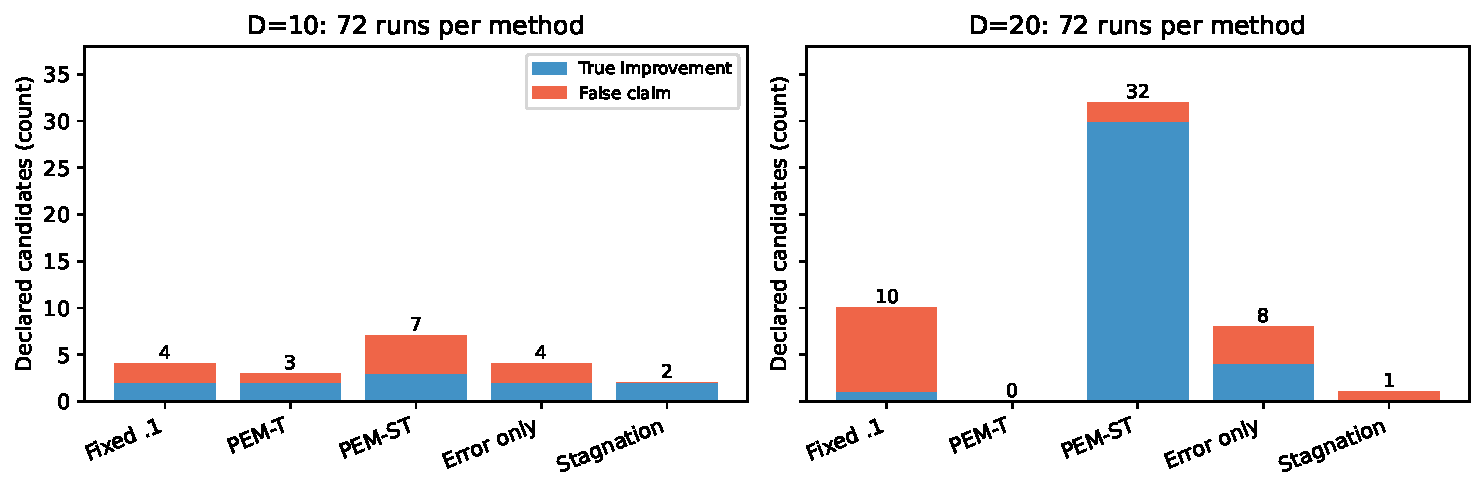
\includegraphics[width=\linewidth,height=.65\textheight,keepaspectratio]{figures/supp_figure_1.pdf}
\caption{Improvement declarations in dimensions 10 (left) and 20 (right), with 72 runs per method and dimension. Blue segments count realized improvements and orange segments count false claims; totals are printed above the bars. A zero column denotes no declarations.}
\end{figure}

Figure S1 exposes both the rarity and composition of improvement declarations. PEM-T makes only three declarations in dimension 10 and none in dimension 20, whereas PEM-ST and the fixed controls produce larger declared subsets. Blue and orange segments distinguish realized improvements from false claims. A missing bar therefore represents an empty conditional sample, while a tall orange segment identifies a declaration rule whose apparent candidates often fail to improve the incumbent.

Failure-only feedback is less detrimental than full feedback on the endpoint summary but still does not achieve an overall benefit over fixed .1. Its combined removal of width and stagnation cannot isolate those terms' independent contributions.

\hypertarget{common-history-diagnostics}{%
\subsection{Common-history diagnostics}\label{common-history-diagnostics}}

Table S2 uses the same T bound within each frozen history/model/pool. Under fixed .3 histories, failures at the actually selected point exceed pool failures. Under greedy histories, their ordering reverses. The observation supports history-dependent differences among monitoring objects and does not support a universal direction of selection-induced undercoverage. Each dimension/history has 288 frozen states; each state contributes one actually selected candidate, 256 pool candidates, and 26 top-10\% candidates.

\FloatBarrier\begingroup\fontsize{8.5}{10.5}\selectfont\setlength\tabcolsep{3pt}

\begin{longtable}[]{@{}
  >{\raggedright\arraybackslash}p{(\columnwidth - 8\tabcolsep) * \real{0.2000}}
  >{\raggedright\arraybackslash}p{(\columnwidth - 8\tabcolsep) * \real{0.2000}}
  >{\raggedright\arraybackslash}p{(\columnwidth - 8\tabcolsep) * \real{0.2000}}
  >{\raggedright\arraybackslash}p{(\columnwidth - 8\tabcolsep) * \real{0.2000}}
  >{\raggedright\arraybackslash}p{(\columnwidth - 8\tabcolsep) * \real{0.2000}}@{}}
\caption{Temporal bounds across monitoring objects}\tabularnewline
\toprule\noalign{}
\begin{minipage}[b]{\linewidth}\raggedright
D
\end{minipage} & \begin{minipage}[b]{\linewidth}\raggedright
History
\end{minipage} & \begin{minipage}[b]{\linewidth}\raggedright
Pool
\end{minipage} & \begin{minipage}[b]{\linewidth}\raggedright
Top 10\%
\end{minipage} & \begin{minipage}[b]{\linewidth}\raggedright
Actually selected
\end{minipage} \\
\midrule\noalign{}
\endfirsthead
\toprule\noalign{}
\begin{minipage}[b]{\linewidth}\raggedright
D
\end{minipage} & \begin{minipage}[b]{\linewidth}\raggedright
History
\end{minipage} & \begin{minipage}[b]{\linewidth}\raggedright
Pool
\end{minipage} & \begin{minipage}[b]{\linewidth}\raggedright
Top 10\%
\end{minipage} & \begin{minipage}[b]{\linewidth}\raggedright
Actually selected
\end{minipage} \\
\midrule\noalign{}
\endhead
\bottomrule\noalign{}
\endlastfoot
10 & fixed03 & 0.0425 & 0.0290 & 0.1250 \\
10 & greedy & 0.1070 & 0.0395 & 0.0868 \\
10 & pool\_\allowbreak random & 0.0773 & 0.0944 & 0.0521 \\
20 & fixed03 & 0.0481 & 0.0423 & 0.1424 \\
20 & greedy & 0.1691 & 0.0843 & 0.0938 \\
20 & pool\_\allowbreak random & 0.0935 & 0.1062 & 0.1042 \\
\end{longtable}

\endgroup

Failure fractions for the selected candidate, full pool, and predicted top 10\% are compared in Figure S2.

\begin{figure}[H]
\centering
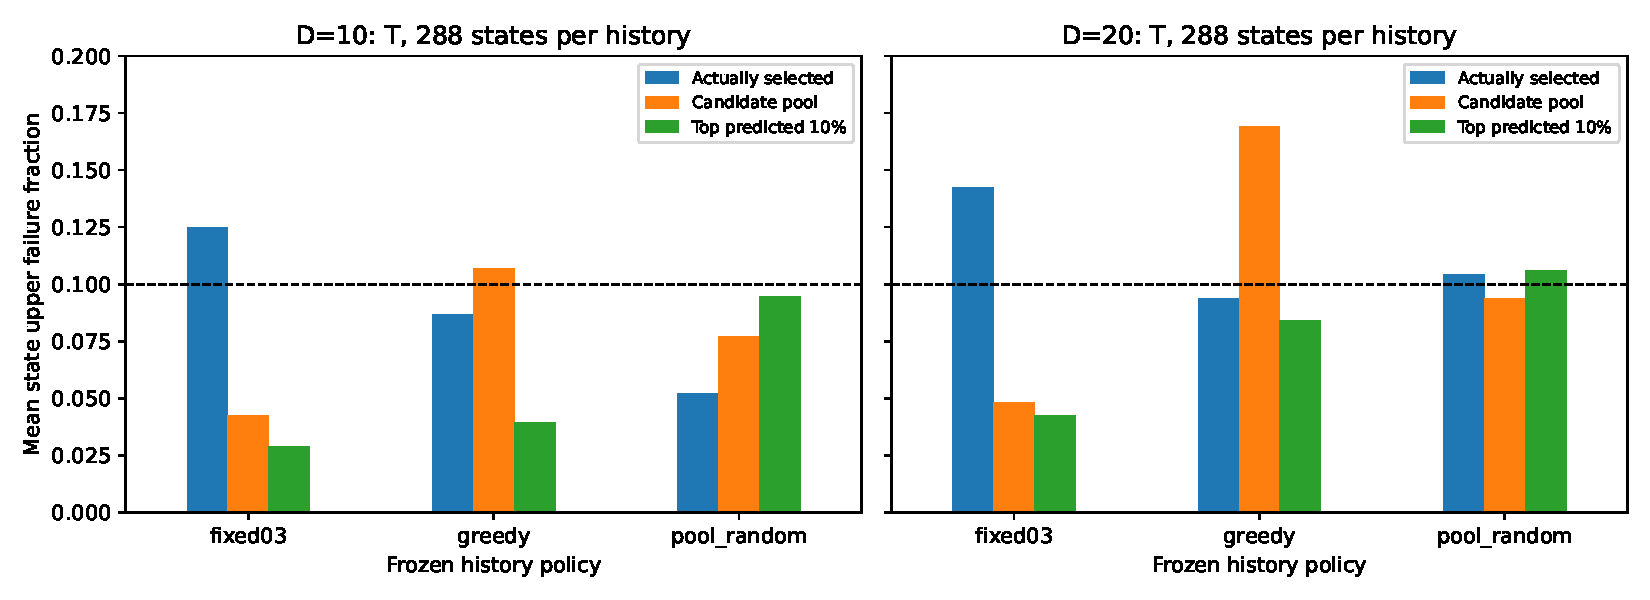
\includegraphics[width=\linewidth,height=.65\textheight,keepaspectratio]{figures/supp_figure_2.pdf}
\caption{State-averaged one-sided failure fractions under frozen common histories, shown separately for dimensions 10 and 20. Blue, orange and green bars denote the selected point, entire pool and top predicted 10\%, respectively. The dashed horizontal line is the target 0.1. Pool labels are correlated.}
\end{figure}

Figure S2 compares three monitored objects at identical frozen states: the actually selected candidate, the entire candidate pool, and the top 10\% by predicted value. Under fixed 03 histories, the selected-candidate bar is highest; under greedy histories, the pool and top-10\% bars become higher. The dashed 0.1 line is crossed in different directions across histories, which supports reporting the monitored object and its generating policy together.

Table S3 compares calibrators on the actually selected points, with the three histories equally weighted. Spatial localization lowers some diagnostic losses and margins; this is a common-history estimation result, not a closed-loop optimization gain or a coverage guarantee. Approximately one quarter of the dimension-10 checkpoint states fall back because of support, whereas these dimension-20 checkpoints do not.

\FloatBarrier\begingroup\fontsize{8.5}{10.5}\selectfont\setlength\tabcolsep{3pt}

\begin{longtable}[]{@{}
  >{\raggedright\arraybackslash}p{(\columnwidth - 10\tabcolsep) * \real{0.1667}}
  >{\raggedright\arraybackslash}p{(\columnwidth - 10\tabcolsep) * \real{0.1667}}
  >{\raggedright\arraybackslash}p{(\columnwidth - 10\tabcolsep) * \real{0.1667}}
  >{\raggedright\arraybackslash}p{(\columnwidth - 10\tabcolsep) * \real{0.1667}}
  >{\raggedright\arraybackslash}p{(\columnwidth - 10\tabcolsep) * \real{0.1667}}
  >{\raggedright\arraybackslash}p{(\columnwidth - 10\tabcolsep) * \real{0.1667}}@{}}
\caption{Calibrators on actually selected points}\tabularnewline
\toprule\noalign{}
\begin{minipage}[b]{\linewidth}\raggedright
D
\end{minipage} & \begin{minipage}[b]{\linewidth}\raggedright
Calibrator
\end{minipage} & \begin{minipage}[b]{\linewidth}\raggedright
Quantile loss
\end{minipage} & \begin{minipage}[b]{\linewidth}\raggedright
Margin
\end{minipage} & \begin{minipage}[b]{\linewidth}\raggedright
ESS
\end{minipage} & \begin{minipage}[b]{\linewidth}\raggedright
Fallback
\end{minipage} \\
\midrule\noalign{}
\endfirsthead
\toprule\noalign{}
\begin{minipage}[b]{\linewidth}\raggedright
D
\end{minipage} & \begin{minipage}[b]{\linewidth}\raggedright
Calibrator
\end{minipage} & \begin{minipage}[b]{\linewidth}\raggedright
Quantile loss
\end{minipage} & \begin{minipage}[b]{\linewidth}\raggedright
Margin
\end{minipage} & \begin{minipage}[b]{\linewidth}\raggedright
ESS
\end{minipage} & \begin{minipage}[b]{\linewidth}\raggedright
Fallback
\end{minipage} \\
\midrule\noalign{}
\endhead
\bottomrule\noalign{}
\endlastfoot
10 & G & 0.1355 & 1.1044 & 45.5000 & 0.0000 \\
10 & S & 0.1241 & 0.9463 & 38.8140 & 0.2500 \\
10 & ST & 0.1187 & 0.9175 & 32.1634 & 0.2500 \\
10 & T & 0.1284 & 1.0262 & 37.7288 & 0.2500 \\
20 & G & 0.1465 & 0.9365 & 74.7500 & 0.0000 \\
20 & S & 0.1322 & 0.7874 & 60.5382 & 0.0000 \\
20 & ST & 0.1307 & 0.7643 & 42.6863 & 0.0000 \\
20 & T & 0.1409 & 0.9114 & 52.3172 & 0.0000 \\
\end{longtable}

\endgroup

Pool-declaration subsets are also sparse: T has only 13 declared candidates under dimension-10 fixed .3 histories, and one under dimension-20 fixed .3 histories. Full state, nonempty-state, candidate, and failure denominators are publicly retained in the diagnostic CSV files. Stable reliability is not inferred from a small or empty subset.

\hypertarget{common-state-immediate-utility}{%
\subsection{Common-state immediate utility}\label{common-state-immediate-utility}}

Table S4 reports normalized true improvement at one chosen candidate from the same frozen pool. T upper-bound selection is identical to mean greedy and is not repeated as an independent column. Full feedback has lower mean immediate improvement than mean greedy and than the predeclared fixed .3 rule in all six dimension/history cells.

\FloatBarrier\begingroup\fontsize{8.5}{10.5}\selectfont\setlength\tabcolsep{3pt}

\begin{longtable}[]{@{}
  >{\raggedright\arraybackslash}p{(\columnwidth - 8\tabcolsep) * \real{0.2000}}
  >{\raggedright\arraybackslash}p{(\columnwidth - 8\tabcolsep) * \real{0.2000}}
  >{\raggedright\arraybackslash}p{(\columnwidth - 8\tabcolsep) * \real{0.2000}}
  >{\raggedright\arraybackslash}p{(\columnwidth - 8\tabcolsep) * \real{0.2000}}
  >{\raggedright\arraybackslash}p{(\columnwidth - 8\tabcolsep) * \real{0.2000}}@{}}
\caption{Common-state normalized one-step improvement}\tabularnewline
\toprule\noalign{}
\begin{minipage}[b]{\linewidth}\raggedright
D
\end{minipage} & \begin{minipage}[b]{\linewidth}\raggedright
History
\end{minipage} & \begin{minipage}[b]{\linewidth}\raggedright
Mean
\end{minipage} & \begin{minipage}[b]{\linewidth}\raggedright
Fixed .3
\end{minipage} & \begin{minipage}[b]{\linewidth}\raggedright
Feedback
\end{minipage} \\
\midrule\noalign{}
\endfirsthead
\toprule\noalign{}
\begin{minipage}[b]{\linewidth}\raggedright
D
\end{minipage} & \begin{minipage}[b]{\linewidth}\raggedright
History
\end{minipage} & \begin{minipage}[b]{\linewidth}\raggedright
Mean
\end{minipage} & \begin{minipage}[b]{\linewidth}\raggedright
Fixed .3
\end{minipage} & \begin{minipage}[b]{\linewidth}\raggedright
Feedback
\end{minipage} \\
\midrule\noalign{}
\endhead
\bottomrule\noalign{}
\endlastfoot
10 & fixed03 & 0.0260 & 0.0219 & 0.0213 \\
10 & greedy & 0.0310 & 0.0257 & 0.0251 \\
10 & pool\_\allowbreak random & 0.1240 & 0.0925 & 0.0867 \\
20 & fixed03 & 0.0350 & 0.0238 & 0.0172 \\
20 & greedy & 0.0541 & 0.0433 & 0.0381 \\
20 & pool\_\allowbreak random & 0.1326 & 0.0871 & 0.0795 \\
\end{longtable}

\endgroup

The closed-loop development experiment also shows no delayed benefit from the additional distance exploration.

\hypertarget{independent-validation-diagnostics-and-external-references}{%
\section{Independent validation diagnostics and external references}\label{independent-validation-diagnostics-and-external-references}}

\hypertarget{history-declarations-and-effective-support}{%
\subsection{History, declarations, and effective support}\label{history-declarations-and-effective-support}}

The history-interaction estimates are D=10: +0.0851 (Holm p=0.00149); D=20: +0.1225 (Holm p=0.00065); D=40: +0.1449 (Holm p=0.00170). This is the fixed .3 selected-minus-pool difference minus the greedy corresponding difference. Across policies, identical seeds do not imply identical candidate pools. These differences describe the coupled history/policy system rather than a fixed-pool causal effect.

\FloatBarrier\begingroup\fontsize{8.5}{10.5}\selectfont\setlength\tabcolsep{3pt}

\begin{longtable}[]{@{}
  >{\raggedright\arraybackslash}p{(\columnwidth - 6\tabcolsep) * \real{0.2500}}
  >{\raggedright\arraybackslash}p{(\columnwidth - 6\tabcolsep) * \real{0.2500}}
  >{\raggedright\arraybackslash}p{(\columnwidth - 6\tabcolsep) * \real{0.2500}}
  >{\raggedright\arraybackslash}p{(\columnwidth - 6\tabcolsep) * \real{0.2500}}@{}}
\caption{Temporal pool and actually selected failure fractions, under the prespecified state/run/instance/function aggregation.}\tabularnewline
\toprule\noalign{}
\begin{minipage}[b]{\linewidth}\raggedright
D
\end{minipage} & \begin{minipage}[b]{\linewidth}\raggedright
History
\end{minipage} & \begin{minipage}[b]{\linewidth}\raggedright
Pool failure
\end{minipage} & \begin{minipage}[b]{\linewidth}\raggedright
Selected failure
\end{minipage} \\
\midrule\noalign{}
\endfirsthead
\toprule\noalign{}
\begin{minipage}[b]{\linewidth}\raggedright
D
\end{minipage} & \begin{minipage}[b]{\linewidth}\raggedright
History
\end{minipage} & \begin{minipage}[b]{\linewidth}\raggedright
Pool failure
\end{minipage} & \begin{minipage}[b]{\linewidth}\raggedright
Selected failure
\end{minipage} \\
\midrule\noalign{}
\endhead
\bottomrule\noalign{}
\endlastfoot
10 & fixed03 & 0.0479 & 0.1215 \\
10 & greedy & 0.1018 & 0.0903 \\
10 & pool\_\allowbreak random & 0.0859 & 0.0660 \\
20 & fixed03 & 0.0442 & 0.0833 \\
20 & greedy & 0.1494 & 0.0660 \\
20 & pool\_\allowbreak random & 0.0900 & 0.0729 \\
40 & fixed03 & 0.0505 & 0.0799 \\
40 & greedy & 0.1850 & 0.0694 \\
40 & pool\_\allowbreak random & 0.0978 & 0.0694 \\
\end{longtable}

\endgroup

The corresponding selected-minus-pool contrasts are shown in Figure S3.

\begin{figure}[H]
\centering
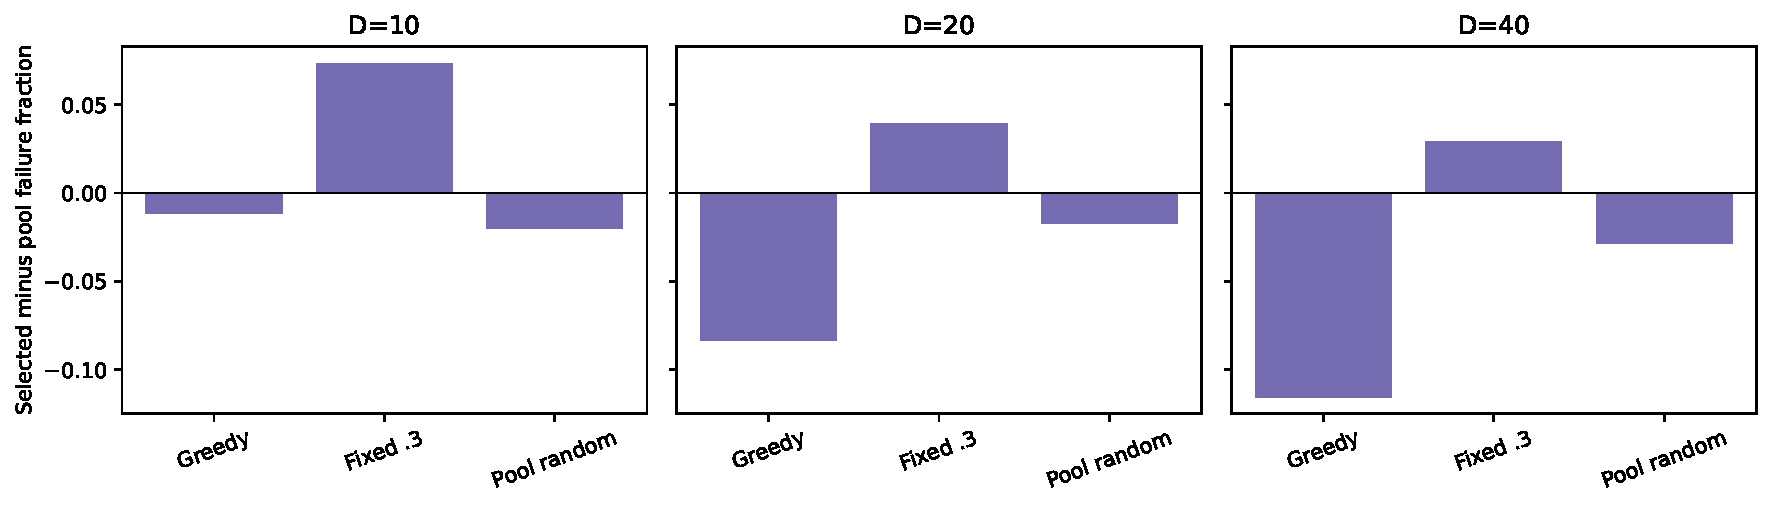
\includegraphics[width=\linewidth,height=.65\textheight,keepaspectratio]{figures/supp_figure_3.pdf}
\caption{Selected-minus-pool failures by preselected history. Positive values indicate greater selected-point failure; negative values indicate lower selected-point failure.}
\end{figure}

Figure S3 expresses the comparison as selected-minus-pool failure fractions in dimensions 10, 20 and 40. The horizontal zero line separates excess selected-point failure from lower selected-point failure. Fixed .3 bars are positive and greedy bars are negative in every panel; the random-pool differences are also negative. The sign reversal between fixed .3 and greedy histories establishes the dependence of selected-point failure on the history-generating policy.

\FloatBarrier\begingroup\fontsize{8.5}{10.5}\selectfont\setlength\tabcolsep{3pt}

\begin{longtable}[]{@{}
  >{\raggedright\arraybackslash}p{(\columnwidth - 12\tabcolsep) * \real{0.1429}}
  >{\raggedright\arraybackslash}p{(\columnwidth - 12\tabcolsep) * \real{0.1429}}
  >{\raggedright\arraybackslash}p{(\columnwidth - 12\tabcolsep) * \real{0.1429}}
  >{\raggedright\arraybackslash}p{(\columnwidth - 12\tabcolsep) * \real{0.1429}}
  >{\raggedright\arraybackslash}p{(\columnwidth - 12\tabcolsep) * \real{0.1429}}
  >{\raggedright\arraybackslash}p{(\columnwidth - 12\tabcolsep) * \real{0.1429}}
  >{\raggedright\arraybackslash}p{(\columnwidth - 12\tabcolsep) * \real{0.1429}}@{}}
\caption{Exploration, failures, and declaration denominators in independent closed-loop runs. FDP is pooled false/claims; no-claim FDP is NA.}\tabularnewline
\toprule\noalign{}
\begin{minipage}[b]{\linewidth}\raggedright
D
\end{minipage} & \begin{minipage}[b]{\linewidth}\raggedright
Method
\end{minipage} & \begin{minipage}[b]{\linewidth}\raggedright
Exploration
\end{minipage} & \begin{minipage}[b]{\linewidth}\raggedright
Failure
\end{minipage} & \begin{minipage}[b]{\linewidth}\raggedright
Claims
\end{minipage} & \begin{minipage}[b]{\linewidth}\raggedright
False
\end{minipage} & \begin{minipage}[b]{\linewidth}\raggedright
Pooled FDP
\end{minipage} \\
\midrule\noalign{}
\endfirsthead
\toprule\noalign{}
\begin{minipage}[b]{\linewidth}\raggedright
D
\end{minipage} & \begin{minipage}[b]{\linewidth}\raggedright
Method
\end{minipage} & \begin{minipage}[b]{\linewidth}\raggedright
Exploration
\end{minipage} & \begin{minipage}[b]{\linewidth}\raggedright
Failure
\end{minipage} & \begin{minipage}[b]{\linewidth}\raggedright
Claims
\end{minipage} & \begin{minipage}[b]{\linewidth}\raggedright
False
\end{minipage} & \begin{minipage}[b]{\linewidth}\raggedright
Pooled FDP
\end{minipage} \\
\midrule\noalign{}
\endhead
\bottomrule\noalign{}
\endlastfoot
10 & PEM\_\allowbreak ST & 0.3936 & 0.1052 & 48 & 23 & 0.4792 \\
10 & PEM\_\allowbreak T & 0.3967 & 0.1008 & 31 & 20 & 0.6452 \\
10 & fixed01 & 0.0949 & 0.0812 & 35 & 21 & 0.6000 \\
20 & PEM\_\allowbreak ST & 0.3687 & 0.1078 & 158 & 36 & 0.2278 \\
20 & PEM\_\allowbreak T & 0.3644 & 0.0942 & 34 & 27 & 0.7941 \\
20 & fixed01 & 0.1018 & 0.0833 & 48 & 32 & 0.6667 \\
40 & PEM\_\allowbreak ST & 0.3701 & 0.1196 & 870 & 98 & 0.1126 \\
40 & PEM\_\allowbreak T & 0.3435 & 0.0964 & 155 & 30 & 0.1935 \\
40 & fixed01 & 0.1007 & 0.0930 & 388 & 71 & 0.1830 \\
\end{longtable}

\endgroup

For PEM-T, D=10: 31 declarations, 20 false, pooled FDP 64.5\%; D=20: 34 declarations, 27 false, pooled FDP 79.4\%; D=40: 155 declarations, 30 false, pooled FDP 19.4\%. An approximately .1 overall failure fraction does not imply an approximately .1 false-declaration fraction. These small declaration denominators do not establish stable per-declaration probabilities. ST lowers the descriptive selected-point quantile loss in all nine dimension/history cells, yet its closed-loop endpoint remains worse than fixed .1 in every dimension. These are separate diagnostic and trajectory comparisons, not an identified causal relationship.

\FloatBarrier\begingroup\fontsize{8.5}{10.5}\selectfont\setlength\tabcolsep{3pt}

\begin{longtable}[]{@{}
  >{\raggedright\arraybackslash}p{(\columnwidth - 6\tabcolsep) * \real{0.2500}}
  >{\raggedright\arraybackslash}p{(\columnwidth - 6\tabcolsep) * \real{0.2500}}
  >{\raggedright\arraybackslash}p{(\columnwidth - 6\tabcolsep) * \real{0.2500}}
  >{\raggedright\arraybackslash}p{(\columnwidth - 6\tabcolsep) * \real{0.2500}}@{}}
\caption{Descriptive state-mean support across the three preselected history policies and four checkpoints.}\tabularnewline
\toprule\noalign{}
\begin{minipage}[b]{\linewidth}\raggedright
D
\end{minipage} & \begin{minipage}[b]{\linewidth}\raggedright
Calibrator
\end{minipage} & \begin{minipage}[b]{\linewidth}\raggedright
State mean ESS
\end{minipage} & \begin{minipage}[b]{\linewidth}\raggedright
State mean fallback
\end{minipage} \\
\midrule\noalign{}
\endfirsthead
\toprule\noalign{}
\begin{minipage}[b]{\linewidth}\raggedright
D
\end{minipage} & \begin{minipage}[b]{\linewidth}\raggedright
Calibrator
\end{minipage} & \begin{minipage}[b]{\linewidth}\raggedright
State mean ESS
\end{minipage} & \begin{minipage}[b]{\linewidth}\raggedright
State mean fallback
\end{minipage} \\
\midrule\noalign{}
\endhead
\bottomrule\noalign{}
\endlastfoot
10 & ST & 32.9284 & 0.2500 \\
10 & T & 37.7288 & 0.2500 \\
20 & ST & 43.6167 & 0.0000 \\
20 & T & 52.3172 & 0.0000 \\
40 & ST & 49.4855 & 0.0004 \\
40 & T & 58.5602 & 0.0000 \\
\end{longtable}

\endgroup

Temporal and spatiotemporal effective support across checkpoint order is shown in Figure S4.

\begin{figure}[H]
\centering
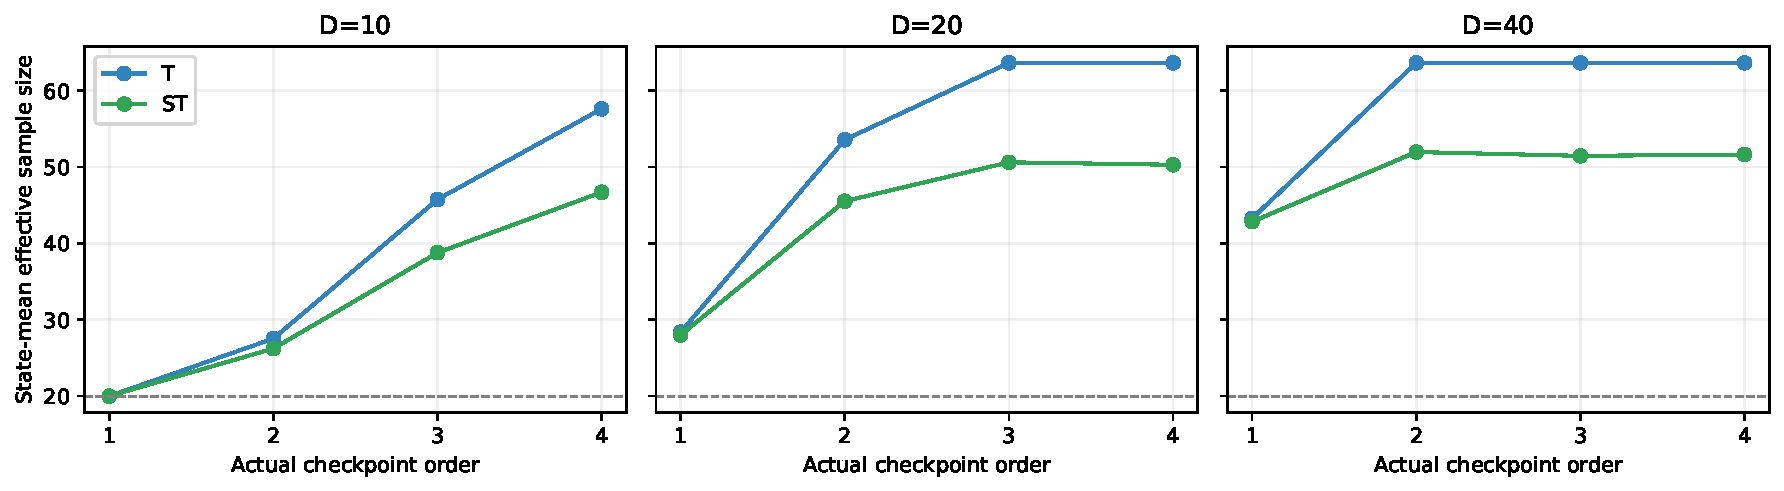
\includegraphics[width=\linewidth,height=.65\textheight,keepaspectratio]{figures/supp_figure_4.pdf}
\caption{Temporal (T, blue) and spatiotemporal (ST, green) effective support in dimensions 10, 20 and 40. The horizontal axis indexes the four actual checkpoints; it is not a common evaluation count across dimensions. The dashed horizontal threshold at 20 is the numerical support guard.}
\end{figure}

Figure S4 shows increasing effective support followed by plateaus in dimensions 20 and 40. More effective observations are retained by T than by ST after spatial localization. In dimension 10, support continues to increase through the fourth checkpoint. Both curves exceed the guard after the earliest checkpoint. The threshold determines eligibility for the localized calculation; calibrated coverage is assessed by the failure diagnostics.

The first diagnostic checkpoints are 41/100, 61/200, and 101/400. Sparse declared-pool subsets disclose nonempty states, candidate counts, and failures separately. Localized quantile-loss, margin, ESS, and fallback differences and the five fixed BBOB structure groups are available in full secondary tables; no favorable subgroup is promoted to a primary result.

\hypertarget{external-background-references}{%
\subsection{External background references}\label{external-background-references}}

Sobol and pycma CMA-ES retain their own search mechanisms and initialization. Their 1,296 runs and 302,400 paid evaluations passed separate journal audits. For descriptive common-scale comparison only, each external run's final error is divided by the matching internal common-initialization error, and medians are taken after this run-level normalization. The external optimizers never receive those internal labels. This supports budget-matched background comparison, not a same-history causal comparison or reproduction of published SAEA competitors.

\FloatBarrier\begingroup\fontsize{8.5}{10.5}\selectfont\setlength\tabcolsep{3pt}

\begin{longtable}[]{@{}
  >{\raggedright\arraybackslash}p{(\columnwidth - 10\tabcolsep) * \real{0.1667}}
  >{\raggedright\arraybackslash}p{(\columnwidth - 10\tabcolsep) * \real{0.1667}}
  >{\raggedright\arraybackslash}p{(\columnwidth - 10\tabcolsep) * \real{0.1667}}
  >{\raggedright\arraybackslash}p{(\columnwidth - 10\tabcolsep) * \real{0.1667}}
  >{\raggedright\arraybackslash}p{(\columnwidth - 10\tabcolsep) * \real{0.1667}}
  >{\raggedright\arraybackslash}p{(\columnwidth - 10\tabcolsep) * \real{0.1667}}@{}}
\caption{Descriptive background endpoint scores over all 24 functions. Lower is better; no additional test family is introduced.}\tabularnewline
\toprule\noalign{}
\begin{minipage}[b]{\linewidth}\raggedright
D
\end{minipage} & \begin{minipage}[b]{\linewidth}\raggedright
Fixed .1
\end{minipage} & \begin{minipage}[b]{\linewidth}\raggedright
PEM-T
\end{minipage} & \begin{minipage}[b]{\linewidth}\raggedright
PEM-ST
\end{minipage} & \begin{minipage}[b]{\linewidth}\raggedright
Sobol
\end{minipage} & \begin{minipage}[b]{\linewidth}\raggedright
CMA-ES
\end{minipage} \\
\midrule\noalign{}
\endfirsthead
\toprule\noalign{}
\begin{minipage}[b]{\linewidth}\raggedright
D
\end{minipage} & \begin{minipage}[b]{\linewidth}\raggedright
Fixed .1
\end{minipage} & \begin{minipage}[b]{\linewidth}\raggedright
PEM-T
\end{minipage} & \begin{minipage}[b]{\linewidth}\raggedright
PEM-ST
\end{minipage} & \begin{minipage}[b]{\linewidth}\raggedright
Sobol
\end{minipage} & \begin{minipage}[b]{\linewidth}\raggedright
CMA-ES
\end{minipage} \\
\midrule\noalign{}
\endhead
\bottomrule\noalign{}
\endlastfoot
10 & -0.8823 & -0.7156 & -0.7465 & -0.0805 & -0.4275 \\
20 & -0.8761 & -0.7763 & -0.7877 & -0.1066 & -0.4799 \\
40 & -0.7934 & -0.7295 & -0.7041 & -0.1029 & -0.4440 \\
\end{longtable}

\endgroup

GP-EI and author TuRBO use separate frozen protocols and strict pre-call budget guards. Their complete audited outcomes are retained in the archived main article. Author-code restart counterexamples are control-flow checks, not performance observations. Resource precheck instances are excluded from every benchmark table.

\hypertarget{complete-bbob-references-and-exclusive-resource-evidence}{%
\section{Complete BBOB references and exclusive resource evidence}\label{complete-bbob-references-and-exclusive-resource-evidence}}

\hypertarget{full-descriptive-bbob-reference-evidence}{%
\subsection{Full descriptive BBOB reference evidence}\label{full-descriptive-bbob-reference-evidence}}

Both frozen GP-EI and author TuRBO-1 batches complete 648 runs and 151,200 paid evaluations each, without reducing functions, repeats, GP training, or acquisition candidates. Together with the six internal and two basic references, all ten methods include 6,480 runs and 1,512,000 paid evaluations. External methods retain their own search and initialization. The matching internal initial-error denominator enters analysis only; normalization precedes within-instance medians. The 24 function scores are equally weighted. These descriptive comparisons add no significance family and do not reproduce the unavailable SAEA competitors.

GP-EI implements classical expected improvement \citep{ref03} using the explicitly frozen kernel and search; it is not an exact reproduction of original EGO software. TuRBO-1 uses the author local trust-region implementation \citep{ref25} with an external paid-call guard.

\FloatBarrier\begingroup\fontsize{8.5}{10.5}\selectfont\setlength\tabcolsep{3pt}

\begin{longtable}[]{@{}
  >{\raggedright\arraybackslash}p{(\columnwidth - 6\tabcolsep) * \real{0.2500}}
  >{\raggedleft\arraybackslash}p{(\columnwidth - 6\tabcolsep) * \real{0.2500}}
  >{\raggedleft\arraybackslash}p{(\columnwidth - 6\tabcolsep) * \real{0.2500}}
  >{\raggedleft\arraybackslash}p{(\columnwidth - 6\tabcolsep) * \real{0.2500}}@{}}
\caption{Full ten-method function-mean log-relative endpoint scores. Lower is better.}\tabularnewline
\toprule\noalign{}
\begin{minipage}[b]{\linewidth}\raggedright
Method
\end{minipage} & \begin{minipage}[b]{\linewidth}\raggedleft
D=10
\end{minipage} & \begin{minipage}[b]{\linewidth}\raggedleft
D=20
\end{minipage} & \begin{minipage}[b]{\linewidth}\raggedleft
D=40
\end{minipage} \\
\midrule\noalign{}
\endfirsthead
\toprule\noalign{}
\begin{minipage}[b]{\linewidth}\raggedright
Method
\end{minipage} & \begin{minipage}[b]{\linewidth}\raggedleft
D=10
\end{minipage} & \begin{minipage}[b]{\linewidth}\raggedleft
D=20
\end{minipage} & \begin{minipage}[b]{\linewidth}\raggedleft
D=40
\end{minipage} \\
\midrule\noalign{}
\endhead
\bottomrule\noalign{}
\endlastfoot
greedy & -0.9152 & -0.9014 & -0.8158 \\
fixed01 & -0.8823 & -0.8761 & -0.7934 \\
fixed03 & -0.7829 & -0.771 & -0.7097 \\
pool\_\allowbreak random & -0.1683 & -0.2223 & -0.2623 \\
PEM\_\allowbreak T & -0.7156 & -0.7763 & -0.7295 \\
PEM\_\allowbreak ST & -0.7465 & -0.7877 & -0.7041 \\
sobol & -0.0805 & -0.1066 & -0.1029 \\
cma\_\allowbreak es & -0.4275 & -0.4799 & -0.444 \\
gp\_\allowbreak ei & -1.3292 & -1.033 & -0.9323 \\
turbo\_\allowbreak 1 & -1.102 & -1.1219 & -1.0389 \\
\end{longtable}

\endgroup

The complete ten-method BBOB endpoint comparison is shown in Figure S5.

\begin{figure}[H]
\centering
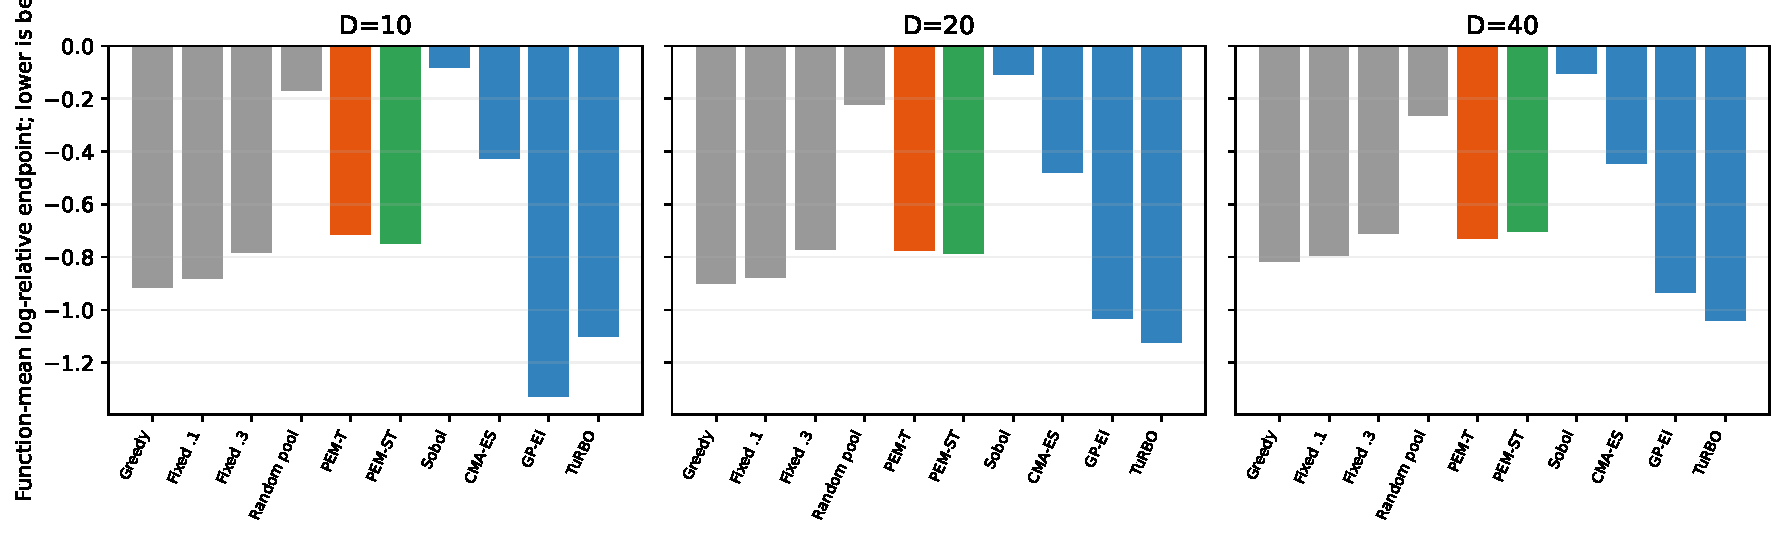
\includegraphics[width=\linewidth,height=.65\textheight,keepaspectratio]{figures/supp_figure_5.pdf}
\caption{Complete BBOB background reference endpoints in dimensions 10, 20 and 40. The vertical quantity is function-mean final $\log_{10}$ relative error, normalized by the matched initial error; lower values indicate greater improvement. Partial runs and resource-precheck instances are excluded.}
\end{figure}

Figure S5 shows four internal controls in grey, PEM-T in orange, PEM-ST in green and four external references in blue. Run-level log-relative endpoints are aggregated by repeat medians, instance means and an equal mean across functions. Negative values indicate reduction relative to the matched initial error. GP-EI and TuRBO-1 have lower aggregate endpoints than the internal configurations, while Sobol remains near zero. The rankings describe the recorded initialization and search protocols.

\hypertarget{exclusive-cost-evidence}{%
\subsection{Exclusive cost evidence}\label{exclusive-cost-evidence}}

The frozen resource design contains 54 fresh, serial process measurements on f1/instance4 across D=10/20/40 and three repeats of six methods. Their 12,600 paid calls are reported as cost observations, excluded from benchmark effect estimation. Actual process and background-CPU guards precede measurements. Runtime includes journaling and each method retains its own initialization. Greedy/fixed controls still perform temporal monitoring, so these are implemented-system costs, not stripped-down ideal algorithm costs.

\FloatBarrier\begingroup\fontsize{8.5}{10.5}\selectfont\setlength\tabcolsep{3pt}

\begin{longtable}[]{@{}
  >{\raggedright\arraybackslash}p{(\columnwidth - 8\tabcolsep) * \real{0.2000}}
  >{\raggedleft\arraybackslash}p{(\columnwidth - 8\tabcolsep) * \real{0.2000}}
  >{\raggedleft\arraybackslash}p{(\columnwidth - 8\tabcolsep) * \real{0.2000}}
  >{\raggedleft\arraybackslash}p{(\columnwidth - 8\tabcolsep) * \real{0.2000}}
  >{\raggedleft\arraybackslash}p{(\columnwidth - 8\tabcolsep) * \real{0.2000}}@{}}
\caption{D=10; three-run medians; full min/max and per-process observations remain in the supplement CSV.}\tabularnewline
\toprule\noalign{}
\begin{minipage}[b]{\linewidth}\raggedright
Method
\end{minipage} & \begin{minipage}[b]{\linewidth}\raggedleft
Algorithm s
\end{minipage} & \begin{minipage}[b]{\linewidth}\raggedleft
Nonobjective s
\end{minipage} & \begin{minipage}[b]{\linewidth}\raggedleft
Peak GiB
\end{minipage} & \begin{minipage}[b]{\linewidth}\raggedleft
Post-init prep s
\end{minipage} \\
\midrule\noalign{}
\endfirsthead
\toprule\noalign{}
\begin{minipage}[b]{\linewidth}\raggedright
Method
\end{minipage} & \begin{minipage}[b]{\linewidth}\raggedleft
Algorithm s
\end{minipage} & \begin{minipage}[b]{\linewidth}\raggedleft
Nonobjective s
\end{minipage} & \begin{minipage}[b]{\linewidth}\raggedleft
Peak GiB
\end{minipage} & \begin{minipage}[b]{\linewidth}\raggedleft
Post-init prep s
\end{minipage} \\
\midrule\noalign{}
\endhead
\bottomrule\noalign{}
\endlastfoot
PEM\_\allowbreak ST & 0.6547 & 0.6543 & 0.0945 & 0.0108 \\
PEM\_\allowbreak T & 0.6075 & 0.6072 & 0.0947 & 0.01 \\
fixed01 & 0.602 & 0.6016 & 0.0947 & 0.0099 \\
gp\_\allowbreak ei & 27.6737 & 27.6724 & 0.2863 & 0.3456 \\
greedy & 0.5983 & 0.5979 & 0.0945 & 0.0098 \\
turbo\_\allowbreak 1 & 7.4536 & 7.4522 & 0.3905 & 0.0923 \\
\end{longtable}

\endgroup

\FloatBarrier\begingroup\fontsize{8.5}{10.5}\selectfont\setlength\tabcolsep{3pt}

\begin{longtable}[]{@{}
  >{\raggedright\arraybackslash}p{(\columnwidth - 8\tabcolsep) * \real{0.2000}}
  >{\raggedleft\arraybackslash}p{(\columnwidth - 8\tabcolsep) * \real{0.2000}}
  >{\raggedleft\arraybackslash}p{(\columnwidth - 8\tabcolsep) * \real{0.2000}}
  >{\raggedleft\arraybackslash}p{(\columnwidth - 8\tabcolsep) * \real{0.2000}}
  >{\raggedleft\arraybackslash}p{(\columnwidth - 8\tabcolsep) * \real{0.2000}}@{}}
\caption{D=20; three-run medians; full min/max and per-process observations remain in the supplement CSV.}\tabularnewline
\toprule\noalign{}
\begin{minipage}[b]{\linewidth}\raggedright
Method
\end{minipage} & \begin{minipage}[b]{\linewidth}\raggedleft
Algorithm s
\end{minipage} & \begin{minipage}[b]{\linewidth}\raggedleft
Nonobjective s
\end{minipage} & \begin{minipage}[b]{\linewidth}\raggedleft
Peak GiB
\end{minipage} & \begin{minipage}[b]{\linewidth}\raggedleft
Post-init prep s
\end{minipage} \\
\midrule\noalign{}
\endfirsthead
\toprule\noalign{}
\begin{minipage}[b]{\linewidth}\raggedright
Method
\end{minipage} & \begin{minipage}[b]{\linewidth}\raggedleft
Algorithm s
\end{minipage} & \begin{minipage}[b]{\linewidth}\raggedleft
Nonobjective s
\end{minipage} & \begin{minipage}[b]{\linewidth}\raggedleft
Peak GiB
\end{minipage} & \begin{minipage}[b]{\linewidth}\raggedleft
Post-init prep s
\end{minipage} \\
\midrule\noalign{}
\endhead
\bottomrule\noalign{}
\endlastfoot
PEM\_\allowbreak ST & 1.6909 & 1.6901 & 0.0946 & 0.012 \\
PEM\_\allowbreak T & 1.5254 & 1.5246 & 0.0948 & 0.0108 \\
fixed01 & 1.5252 & 1.5244 & 0.0948 & 0.0108 \\
gp\_\allowbreak ei & 175.864 & 175.861 & 0.3059 & 1.0989 \\
greedy & 1.5246 & 1.5238 & 0.0945 & 0.0108 \\
turbo\_\allowbreak 1 & 35.0159 & 35.013 & 0.5936 & 0.2183 \\
\end{longtable}

\endgroup

\FloatBarrier\begingroup\fontsize{8.5}{10.5}\selectfont\setlength\tabcolsep{3pt}

\begin{longtable}[]{@{}
  >{\raggedright\arraybackslash}p{(\columnwidth - 8\tabcolsep) * \real{0.2000}}
  >{\raggedleft\arraybackslash}p{(\columnwidth - 8\tabcolsep) * \real{0.2000}}
  >{\raggedleft\arraybackslash}p{(\columnwidth - 8\tabcolsep) * \real{0.2000}}
  >{\raggedleft\arraybackslash}p{(\columnwidth - 8\tabcolsep) * \real{0.2000}}
  >{\raggedleft\arraybackslash}p{(\columnwidth - 8\tabcolsep) * \real{0.2000}}@{}}
\caption{D=40; three-run medians; full min/max and per-process observations remain in the supplement CSV.}\tabularnewline
\toprule\noalign{}
\begin{minipage}[b]{\linewidth}\raggedright
Method
\end{minipage} & \begin{minipage}[b]{\linewidth}\raggedleft
Algorithm s
\end{minipage} & \begin{minipage}[b]{\linewidth}\raggedleft
Nonobjective s
\end{minipage} & \begin{minipage}[b]{\linewidth}\raggedleft
Peak GiB
\end{minipage} & \begin{minipage}[b]{\linewidth}\raggedleft
Post-init prep s
\end{minipage} \\
\midrule\noalign{}
\endfirsthead
\toprule\noalign{}
\begin{minipage}[b]{\linewidth}\raggedright
Method
\end{minipage} & \begin{minipage}[b]{\linewidth}\raggedleft
Algorithm s
\end{minipage} & \begin{minipage}[b]{\linewidth}\raggedleft
Nonobjective s
\end{minipage} & \begin{minipage}[b]{\linewidth}\raggedleft
Peak GiB
\end{minipage} & \begin{minipage}[b]{\linewidth}\raggedleft
Post-init prep s
\end{minipage} \\
\midrule\noalign{}
\endhead
\bottomrule\noalign{}
\endlastfoot
PEM\_\allowbreak ST & 4.7496 & 4.7476 & 0.096 & 0.0157 \\
PEM\_\allowbreak T & 4.3878 & 4.3856 & 0.0962 & 0.0145 \\
fixed01 & 4.3787 & 4.3766 & 0.0965 & 0.0145 \\
gp\_\allowbreak ei & 1308.81 & 1308.8 & 0.3073 & 4.0897 \\
greedy & 4.3615 & 4.3594 & 0.0958 & 0.0144 \\
turbo\_\allowbreak 1 & 255.912 & 255.906 & 1.0791 & 0.7993 \\
\end{longtable}

\endgroup

The measured-overhead and assumed-objective-cost scenarios are shown in Figure S6.

\begin{figure}[H]
\centering
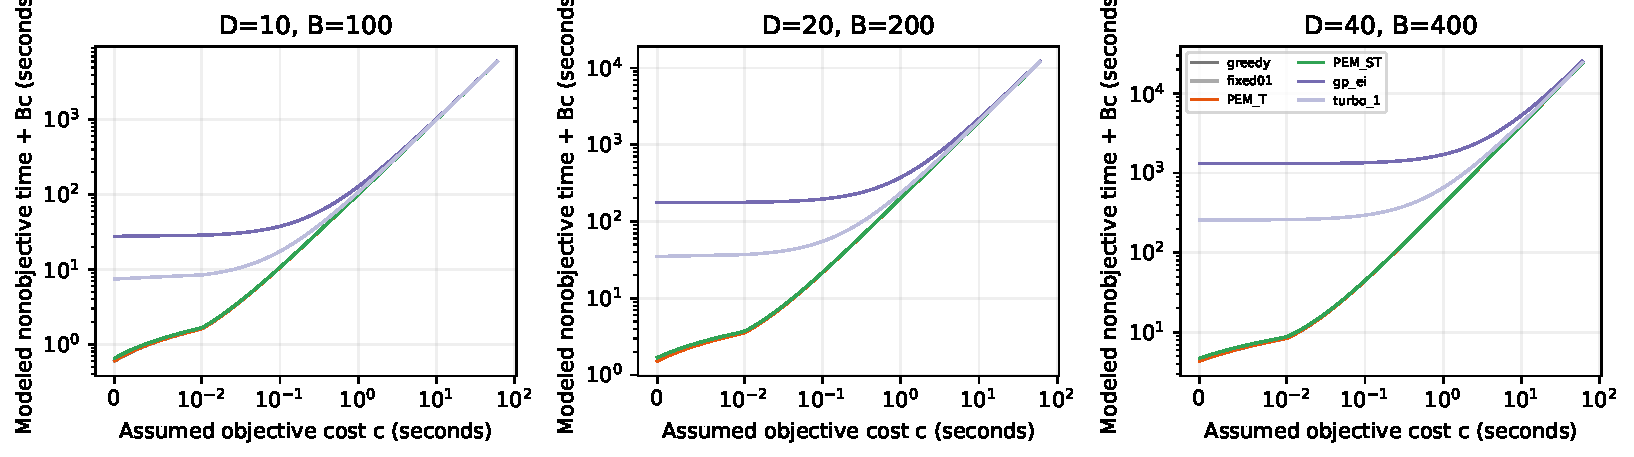
\includegraphics[width=\linewidth,height=.65\textheight,keepaspectratio]{figures/supp_figure_6.pdf}
\caption{Objective-cost scenarios from serial measurements for $D=10,20,40$, with $B=100,200,400$, respectively. Total modeled time is measured nonobjective time plus $Bc$, in seconds. The horizontal axis is linear for $0\leq c\leq0.01$ s and logarithmic above 0.01 s; the vertical axis is logarithmic. All methods use the same $B$ within a panel.}
\end{figure}

Figure S6 separates measured algorithm overhead from an assumed per-evaluation objective cost. At $c=0$, each curve reports the measured nonobjective-time contribution; the largest overheads occur for GP-EI and TuRBO-1. The gaps narrow as the shared $Bc$ term dominates at higher objective cost. Curve convergence therefore reflects the equal paid-evaluation budget in each dimension. No parallel execution was measured in these scenarios.

At an assumed objective cost c, total time is modeled as measured nonobjective time plus Bc. This scenario is not an observed application acceleration. Equal evaluation budgets have equal objective-cost slopes and cannot establish evaluation savings.

\hypertarget{lassobench-application-transfer}{%
\section{LassoBench application transfer}\label{lassobench-application-transfer}}

\hypertarget{lassobench-mechanism-transfer}{%
\subsection{LassoBench mechanism transfer}\label{lassobench-mechanism-transfer}}

LassoBench \citep{ref24} provides the application objectives. A separate protocol is frozen before formal seed42 labels. Three original tasks (D=60/100/180), eight methods, twenty optimization repeats, and 500 evaluations yield 480 runs and 240,000 full configuration evaluations (1,200,000 CV-fold solves). Internal initialization is 140/220/380 paid calls; external initialization remains native. The author five-fold full-fidelity objective, fixed data/splits, solver settings, bounds, and target definitions are unchanged.

Unknown optimum is never imputed. The main endpoint is original validation loss. After all 500 labels are saved, the first lowest-validation configuration receives exactly one author test call, adding 480 single fits separately. Synthetic test MSPE uses the author fixed oracle normalizer, while DNA uses absolute test MSE; these scales are not pooled. The synthetic constructor computes its fixed test normalizer, but no test-performance result enters any optimization feedback.

\FloatBarrier\begingroup\fontsize{8.5}{10.5}\selectfont\setlength\tabcolsep{3pt}

\begin{longtable}[]{@{}
  >{\raggedright\arraybackslash}p{(\columnwidth - 10\tabcolsep) * \real{0.1667}}
  >{\raggedleft\arraybackslash}p{(\columnwidth - 10\tabcolsep) * \real{0.1667}}
  >{\raggedleft\arraybackslash}p{(\columnwidth - 10\tabcolsep) * \real{0.1667}}
  >{\raggedleft\arraybackslash}p{(\columnwidth - 10\tabcolsep) * \real{0.1667}}
  >{\raggedleft\arraybackslash}p{(\columnwidth - 10\tabcolsep) * \real{0.1667}}
  >{\raggedleft\arraybackslash}p{(\columnwidth - 10\tabcolsep) * \real{0.1667}}@{}}
\caption{synt\_\allowbreak simple; twenty optimization-run dispersion and post-completion test medians.}\tabularnewline
\toprule\noalign{}
\begin{minipage}[b]{\linewidth}\raggedright
Method
\end{minipage} & \begin{minipage}[b]{\linewidth}\raggedleft
CV median
\end{minipage} & \begin{minipage}[b]{\linewidth}\raggedleft
Q1
\end{minipage} & \begin{minipage}[b]{\linewidth}\raggedleft
Q3
\end{minipage} & \begin{minipage}[b]{\linewidth}\raggedleft
Test MSPE median
\end{minipage} & \begin{minipage}[b]{\linewidth}\raggedleft
F-score median
\end{minipage} \\
\midrule\noalign{}
\endfirsthead
\toprule\noalign{}
\begin{minipage}[b]{\linewidth}\raggedright
Method
\end{minipage} & \begin{minipage}[b]{\linewidth}\raggedleft
CV median
\end{minipage} & \begin{minipage}[b]{\linewidth}\raggedleft
Q1
\end{minipage} & \begin{minipage}[b]{\linewidth}\raggedleft
Q3
\end{minipage} & \begin{minipage}[b]{\linewidth}\raggedleft
Test MSPE median
\end{minipage} & \begin{minipage}[b]{\linewidth}\raggedleft
F-score median
\end{minipage} \\
\midrule\noalign{}
\endhead
\bottomrule\noalign{}
\endlastfoot
PEM\_\allowbreak ST & 0.7896 & 0.7656 & 0.8528 & 1.1435 & 0.6667 \\
PEM\_\allowbreak T & 0.7714 & 0.7557 & 0.8654 & 1.2013 & 0.6667 \\
cma\_\allowbreak es & 0.758 & 0.7176 & 0.7826 & 1.072 & 0.5455 \\
fixed01 & 0.7534 & 0.7092 & 0.816 & 1.1441 & 0.6667 \\
gp\_\allowbreak ei & 1.0118 & 0.9392 & 1.0847 & 1.1167 & 0.6 \\
greedy & 0.7501 & 0.703 & 0.7755 & 1.1078 & 0.6 \\
sobol & 1.2057 & 1.0326 & 1.2544 & 1.1865 & 0.4808 \\
turbo\_\allowbreak 1 & 0.6448 & 0.5888 & 0.7032 & 1.0643 & 0.6 \\
\end{longtable}

\endgroup

\FloatBarrier\begingroup\fontsize{8.5}{10.5}\selectfont\setlength\tabcolsep{3pt}

\begin{longtable}[]{@{}
  >{\raggedright\arraybackslash}p{(\columnwidth - 10\tabcolsep) * \real{0.1667}}
  >{\raggedleft\arraybackslash}p{(\columnwidth - 10\tabcolsep) * \real{0.1667}}
  >{\raggedleft\arraybackslash}p{(\columnwidth - 10\tabcolsep) * \real{0.1667}}
  >{\raggedleft\arraybackslash}p{(\columnwidth - 10\tabcolsep) * \real{0.1667}}
  >{\raggedleft\arraybackslash}p{(\columnwidth - 10\tabcolsep) * \real{0.1667}}
  >{\raggedleft\arraybackslash}p{(\columnwidth - 10\tabcolsep) * \real{0.1667}}@{}}
\caption{synt\_\allowbreak medium; twenty optimization-run dispersion and post-completion test medians.}\tabularnewline
\toprule\noalign{}
\begin{minipage}[b]{\linewidth}\raggedright
Method
\end{minipage} & \begin{minipage}[b]{\linewidth}\raggedleft
CV median
\end{minipage} & \begin{minipage}[b]{\linewidth}\raggedleft
Q1
\end{minipage} & \begin{minipage}[b]{\linewidth}\raggedleft
Q3
\end{minipage} & \begin{minipage}[b]{\linewidth}\raggedleft
Test MSPE median
\end{minipage} & \begin{minipage}[b]{\linewidth}\raggedleft
F-score median
\end{minipage} \\
\midrule\noalign{}
\endfirsthead
\toprule\noalign{}
\begin{minipage}[b]{\linewidth}\raggedright
Method
\end{minipage} & \begin{minipage}[b]{\linewidth}\raggedleft
CV median
\end{minipage} & \begin{minipage}[b]{\linewidth}\raggedleft
Q1
\end{minipage} & \begin{minipage}[b]{\linewidth}\raggedleft
Q3
\end{minipage} & \begin{minipage}[b]{\linewidth}\raggedleft
Test MSPE median
\end{minipage} & \begin{minipage}[b]{\linewidth}\raggedleft
F-score median
\end{minipage} \\
\midrule\noalign{}
\endhead
\bottomrule\noalign{}
\endlastfoot
PEM\_\allowbreak ST & 1.146 & 1.1122 & 1.1731 & 0.7697 & 0.7692 \\
PEM\_\allowbreak T & 1.1519 & 1.1327 & 1.1684 & 0.7562 & 0.8013 \\
cma\_\allowbreak es & 1.1888 & 1.1345 & 1.237 & 0.7927 & 0.625 \\
fixed01 & 1.1186 & 1.0751 & 1.1418 & 0.7486 & 0.7692 \\
gp\_\allowbreak ei & 1.61 & 1.5226 & 1.7486 & 0.8469 & 0.6667 \\
greedy & 1.1103 & 1.069 & 1.1616 & 0.7703 & 0.7692 \\
sobol & 1.8953 & 1.7099 & 2.0302 & 0.8846 & 0.625 \\
turbo\_\allowbreak 1 & 1.0277 & 0.9575 & 1.0632 & 0.835 & 0.625 \\
\end{longtable}

\endgroup

\FloatBarrier\begingroup\fontsize{8.5}{10.5}\selectfont\setlength\tabcolsep{3pt}

\begin{longtable}[]{@{}
  >{\raggedright\arraybackslash}p{(\columnwidth - 10\tabcolsep) * \real{0.1667}}
  >{\raggedleft\arraybackslash}p{(\columnwidth - 10\tabcolsep) * \real{0.1667}}
  >{\raggedleft\arraybackslash}p{(\columnwidth - 10\tabcolsep) * \real{0.1667}}
  >{\raggedleft\arraybackslash}p{(\columnwidth - 10\tabcolsep) * \real{0.1667}}
  >{\raggedleft\arraybackslash}p{(\columnwidth - 10\tabcolsep) * \real{0.1667}}
  >{\raggedright\arraybackslash}p{(\columnwidth - 10\tabcolsep) * \real{0.1667}}@{}}
\caption{DNA; twenty optimization-run dispersion and post-completion test medians.}\tabularnewline
\toprule\noalign{}
\begin{minipage}[b]{\linewidth}\raggedright
Method
\end{minipage} & \begin{minipage}[b]{\linewidth}\raggedleft
CV median
\end{minipage} & \begin{minipage}[b]{\linewidth}\raggedleft
Q1
\end{minipage} & \begin{minipage}[b]{\linewidth}\raggedleft
Q3
\end{minipage} & \begin{minipage}[b]{\linewidth}\raggedleft
Test MSPE median
\end{minipage} & \begin{minipage}[b]{\linewidth}\raggedright
F-score median
\end{minipage} \\
\midrule\noalign{}
\endfirsthead
\toprule\noalign{}
\begin{minipage}[b]{\linewidth}\raggedright
Method
\end{minipage} & \begin{minipage}[b]{\linewidth}\raggedleft
CV median
\end{minipage} & \begin{minipage}[b]{\linewidth}\raggedleft
Q1
\end{minipage} & \begin{minipage}[b]{\linewidth}\raggedleft
Q3
\end{minipage} & \begin{minipage}[b]{\linewidth}\raggedleft
Test MSPE median
\end{minipage} & \begin{minipage}[b]{\linewidth}\raggedright
F-score median
\end{minipage} \\
\midrule\noalign{}
\endhead
\bottomrule\noalign{}
\endlastfoot
PEM\_\allowbreak ST & 0.3071 & 0.3056 & 0.3092 & 0.3304 & NA \\
PEM\_\allowbreak T & 0.3073 & 0.3054 & 0.3093 & 0.3277 & NA \\
cma\_\allowbreak es & 0.3014 & 0.2992 & 0.3043 & 0.3285 & NA \\
fixed01 & 0.306 & 0.3025 & 0.3079 & 0.3307 & NA \\
gp\_\allowbreak ei & 0.336 & 0.3328 & 0.3384 & 0.3495 & NA \\
greedy & 0.3057 & 0.3042 & 0.3067 & 0.327 & NA \\
sobol & 0.3348 & 0.332 & 0.3375 & 0.3439 & NA \\
turbo\_\allowbreak 1 & 0.3028 & 0.3005 & 0.3052 & 0.3278 & NA \\
\end{longtable}

\endgroup

\FloatBarrier\begingroup\fontsize{8.5}{10.5}\selectfont\setlength\tabcolsep{3pt}

\begin{longtable}[]{@{}
  >{\raggedright\arraybackslash}p{(\columnwidth - 14\tabcolsep) * \real{0.1250}}
  >{\raggedleft\arraybackslash}p{(\columnwidth - 14\tabcolsep) * \real{0.1250}}
  >{\raggedleft\arraybackslash}p{(\columnwidth - 14\tabcolsep) * \real{0.1250}}
  >{\raggedleft\arraybackslash}p{(\columnwidth - 14\tabcolsep) * \real{0.1250}}
  >{\raggedleft\arraybackslash}p{(\columnwidth - 14\tabcolsep) * \real{0.1250}}
  >{\raggedleft\arraybackslash}p{(\columnwidth - 14\tabcolsep) * \real{0.1250}}
  >{\raggedleft\arraybackslash}p{(\columnwidth - 14\tabcolsep) * \real{0.1250}}
  >{\raggedleft\arraybackslash}p{(\columnwidth - 14\tabcolsep) * \real{0.1250}}@{}}
\caption{Prespecified application family, PEM-T minus fixed .1 raw final validation loss. Positive favors the fixed control. Intervals are unadjusted paired-run bootstrap.}\tabularnewline
\toprule\noalign{}
\begin{minipage}[b]{\linewidth}\raggedright
Task
\end{minipage} & \begin{minipage}[b]{\linewidth}\raggedleft
Median difference
\end{minipage} & \begin{minipage}[b]{\linewidth}\raggedleft
CI low
\end{minipage} & \begin{minipage}[b]{\linewidth}\raggedleft
CI high
\end{minipage} & \begin{minipage}[b]{\linewidth}\raggedleft
Holm p
\end{minipage} & \begin{minipage}[b]{\linewidth}\raggedleft
Loss
\end{minipage} & \begin{minipage}[b]{\linewidth}\raggedleft
Win
\end{minipage} & \begin{minipage}[b]{\linewidth}\raggedleft
Tie
\end{minipage} \\
\midrule\noalign{}
\endfirsthead
\toprule\noalign{}
\begin{minipage}[b]{\linewidth}\raggedright
Task
\end{minipage} & \begin{minipage}[b]{\linewidth}\raggedleft
Median difference
\end{minipage} & \begin{minipage}[b]{\linewidth}\raggedleft
CI low
\end{minipage} & \begin{minipage}[b]{\linewidth}\raggedleft
CI high
\end{minipage} & \begin{minipage}[b]{\linewidth}\raggedleft
Holm p
\end{minipage} & \begin{minipage}[b]{\linewidth}\raggedleft
Loss
\end{minipage} & \begin{minipage}[b]{\linewidth}\raggedleft
Win
\end{minipage} & \begin{minipage}[b]{\linewidth}\raggedleft
Tie
\end{minipage} \\
\midrule\noalign{}
\endhead
\bottomrule\noalign{}
\endlastfoot
synt\_\allowbreak simple & 0.0503 & 0.0032 & 0.0725 & 0.0826 & 14 & 6 & 0 \\
synt\_\allowbreak medium & 0.0393 & 0.0221 & 0.0626 & 0.0192 & 16 & 4 & 0 \\
DNA & 0.0027 & 0.0005279 & 0.0044 & 0.0592 & 16 & 4 & 0 \\
\end{longtable}

\endgroup

synt\_\allowbreak simple: higher, Holm p=0.0826; synt\_\allowbreak medium: higher, Holm p=0.0192; DNA: higher, Holm p=0.0592.

The three comparisons form an application-only Holm family, separate from the nine BBOB mechanism tests. Twenty repeats describe optimization randomness on one fixed dataset and split per task, not twenty independent datasets. The Wilcoxon and paired bootstrap analyses condition on the fixed task data and split.

Original-scale validation endpoints for the three LassoBench tasks are shown in Figure S7.

\begin{figure}[H]
\centering
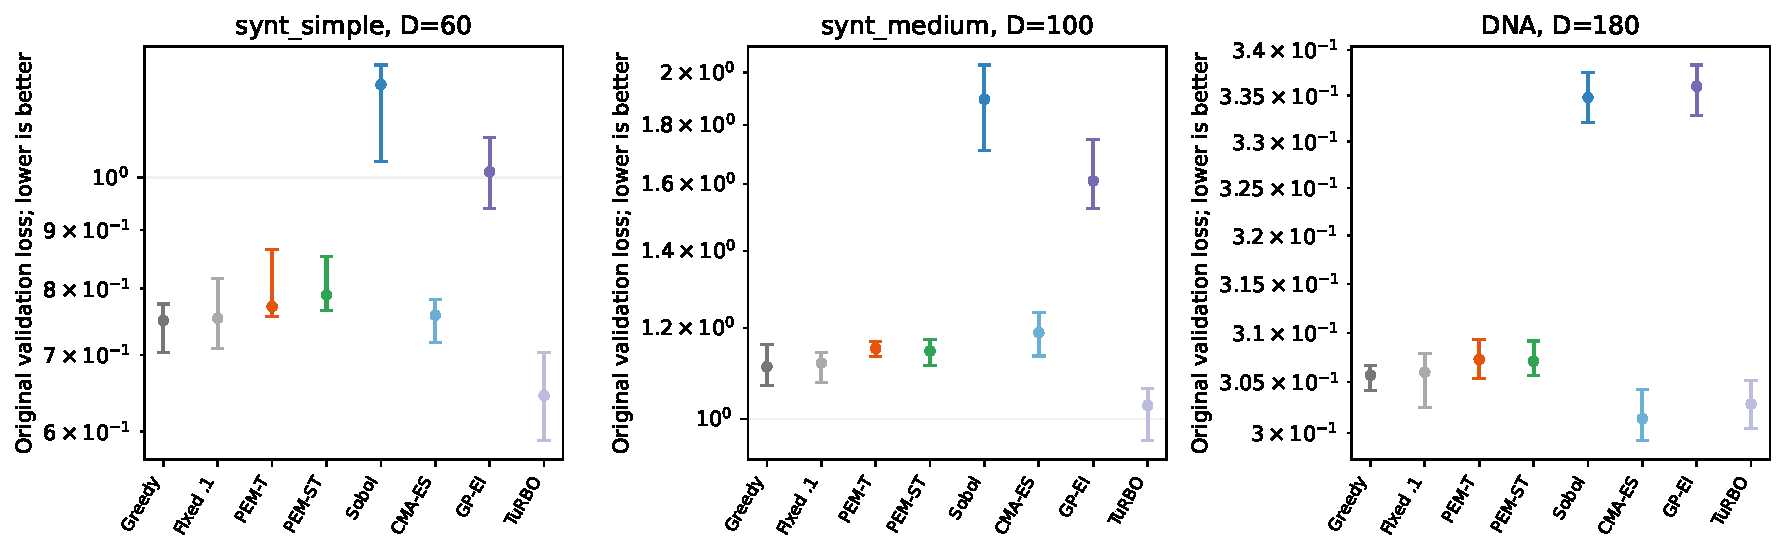
\includegraphics[width=\linewidth,height=.65\textheight,keepaspectratio]{figures/supp_figure_7.pdf}
\caption{LassoBench validation-loss endpoints for synt\_simple ($D=60$), synt\_medium ($D=100$) and DNA ($D=180$). Points show run medians and vertical bars span the 25th--75th percentiles. Each vertical axis is logarithmic in original validation-loss units; lower is better.}
\end{figure}

Figure S7 reports task-specific original validation losses, with a separate vertical range for each task. The synthetic-task panels separate the lower-loss internal and trust-region configurations from Sobol and GP-EI, whereas DNA endpoints occupy a narrower relative range. The bars describe dispersion across runs and are not confidence intervals for the median. Loss magnitudes are compared within each task.

Their median and interquartile convergence histories are shown in Figure S8.

\begin{figure}[H]
\centering
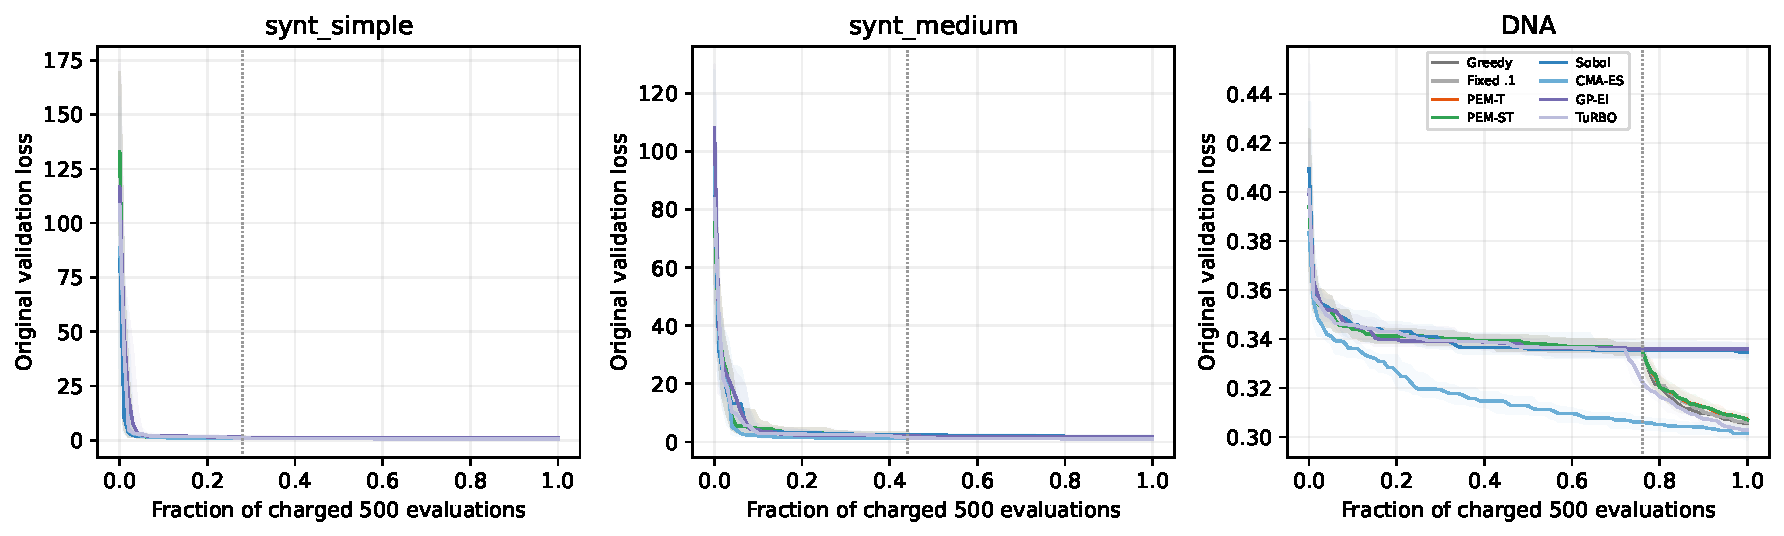
\includegraphics[width=\linewidth,height=.65\textheight,keepaspectratio]{figures/supp_figure_8.pdf}
\caption{Original validation-loss convergence under the charged 500-evaluation budget. Lines show run medians and shaded bands span the 25th--75th percentiles. The dotted vertical lines mark internal initialization at budget fractions 0.28, 0.44 and 0.76, respectively; external designs differ. Zero fraction displays the first paid label.}
\end{figure}

Figure S8 uses a linear validation-loss axis, so the large early reductions on the synthetic tasks compress later differences. The internal initialization costs are 140, 220 and 380 paid evaluations for synt\_\allowbreak simple, synt\_\allowbreak medium and DNA, respectively. The long DNA initialization occupies most of the horizontal range; postinitial changes occur to the right of its dotted boundary. External curves retain their own initialization and search histories.

\FloatBarrier\begingroup\fontsize{8.5}{10.5}\selectfont\setlength\tabcolsep{3pt}

\begin{longtable}[]{@{}
  >{\raggedright\arraybackslash}p{(\columnwidth - 14\tabcolsep) * \real{0.1250}}
  >{\raggedright\arraybackslash}p{(\columnwidth - 14\tabcolsep) * \real{0.1250}}
  >{\raggedleft\arraybackslash}p{(\columnwidth - 14\tabcolsep) * \real{0.1250}}
  >{\raggedleft\arraybackslash}p{(\columnwidth - 14\tabcolsep) * \real{0.1250}}
  >{\raggedleft\arraybackslash}p{(\columnwidth - 14\tabcolsep) * \real{0.1250}}
  >{\raggedleft\arraybackslash}p{(\columnwidth - 14\tabcolsep) * \real{0.1250}}
  >{\raggedright\arraybackslash}p{(\columnwidth - 14\tabcolsep) * \real{0.1250}}
  >{\raggedleft\arraybackslash}p{(\columnwidth - 14\tabcolsep) * \real{0.1250}}@{}}
\caption{Descriptive post-initialization selected-point monitoring; no hidden pool objectives are acquired.}\tabularnewline
\toprule\noalign{}
\begin{minipage}[b]{\linewidth}\raggedright
Task
\end{minipage} & \begin{minipage}[b]{\linewidth}\raggedright
Method
\end{minipage} & \begin{minipage}[b]{\linewidth}\raggedleft
Failure
\end{minipage} & \begin{minipage}[b]{\linewidth}\raggedleft
Q-loss
\end{minipage} & \begin{minipage}[b]{\linewidth}\raggedleft
Claims
\end{minipage} & \begin{minipage}[b]{\linewidth}\raggedleft
False
\end{minipage} & \begin{minipage}[b]{\linewidth}\raggedright
Pooled FDP
\end{minipage} & \begin{minipage}[b]{\linewidth}\raggedleft
No-claim runs
\end{minipage} \\
\midrule\noalign{}
\endfirsthead
\toprule\noalign{}
\begin{minipage}[b]{\linewidth}\raggedright
Task
\end{minipage} & \begin{minipage}[b]{\linewidth}\raggedright
Method
\end{minipage} & \begin{minipage}[b]{\linewidth}\raggedleft
Failure
\end{minipage} & \begin{minipage}[b]{\linewidth}\raggedleft
Q-loss
\end{minipage} & \begin{minipage}[b]{\linewidth}\raggedleft
Claims
\end{minipage} & \begin{minipage}[b]{\linewidth}\raggedleft
False
\end{minipage} & \begin{minipage}[b]{\linewidth}\raggedright
Pooled FDP
\end{minipage} & \begin{minipage}[b]{\linewidth}\raggedleft
No-claim runs
\end{minipage} \\
\midrule\noalign{}
\endhead
\bottomrule\noalign{}
\endlastfoot
DNA & PEM\_\allowbreak ST & 0.0704 & 0.0698 & 0 & 0 & NA & 20 \\
DNA & PEM\_\allowbreak T & 0.0629 & 0.084 & 0 & 0 & NA & 20 \\
DNA & fixed01 & 0.0346 & 0.0627 & 0 & 0 & NA & 20 \\
DNA & greedy & 0.0079 & 0.041 & 1 & 1 & 1.0000 & 19 \\
synt\_\allowbreak medium & PEM\_\allowbreak ST & 0.1036 & 0.0778 & 53 & 46 & 0.8679 & 1 \\
synt\_\allowbreak medium & PEM\_\allowbreak T & 0.0887 & 0.0904 & 7 & 6 & 0.8571 & 14 \\
synt\_\allowbreak medium & fixed01 & 0.0505 & 0.0452 & 27 & 23 & 0.8519 & 5 \\
synt\_\allowbreak medium & greedy & 0.0134 & 0.0147 & 60 & 54 & 0.9000 & 1 \\
synt\_\allowbreak simple & PEM\_\allowbreak ST & 0.1103 & 0.0946 & 75 & 74 & 0.9867 & 1 \\
synt\_\allowbreak simple & PEM\_\allowbreak T & 0.0931 & 0.1104 & 7 & 6 & 0.8571 & 15 \\
synt\_\allowbreak simple & fixed01 & 0.0549 & 0.0476 & 76 & 74 & 0.9737 & 1 \\
synt\_\allowbreak simple & greedy & 0.0367 & 0.0137 & 220 & 218 & 0.9909 & 0 \\
\end{longtable}

\endgroup

These closed-loop histories differ between methods and do not identify same-pool causal effects. Zero declarations give NA FDP, with counts disclosed. The 300-dimensional synt\_\allowbreak high extension therefore uses its separately frozen 1,000-evaluation protocol, reported in Section S5. Application findings cannot undo the failed original development gate.

\hypertarget{predefined-300-dimensional-extension}{%
\section{Predefined 300-dimensional extension}\label{predefined-300-dimensional-extension}}

The predefined synt\_\allowbreak high extension used 1,000 paid evaluations because the unchanged internal initialization requires 620, exceeding the 500-evaluation primary-application budget. Eight methods completed 20 optimization runs on one fixed seed42 data set and split (160 runs; 160,000 validation evaluations; 800,000 CV-fold solves), followed by exactly one held-out test call per completed run. The low-effective-dimensional synthetic construction and different budget preclude a general high-dimensional or cross-task superiority claim.

\hypertarget{endpoints-and-convergence}{%
\subsection{Endpoints and convergence}\label{endpoints-and-convergence}}

\FloatBarrier\begingroup\fontsize{8.5}{10.5}\selectfont\setlength\tabcolsep{3pt}

\begin{longtable}[]{@{}
  >{\raggedright\arraybackslash}p{(\columnwidth - 6\tabcolsep) * \real{0.2500}}
  >{\raggedright\arraybackslash}p{(\columnwidth - 6\tabcolsep) * \real{0.2500}}
  >{\raggedright\arraybackslash}p{(\columnwidth - 6\tabcolsep) * \real{0.2500}}
  >{\raggedright\arraybackslash}p{(\columnwidth - 6\tabcolsep) * \real{0.2500}}@{}}
\caption{Endpoints and convergence.}\tabularnewline
\toprule\noalign{}
\begin{minipage}[b]{\linewidth}\raggedright
Method
\end{minipage} & \begin{minipage}[b]{\linewidth}\raggedright
Validation median {[}Q1, Q3{]}
\end{minipage} & \begin{minipage}[b]{\linewidth}\raggedright
Test MSPE median {[}Q1, Q3{]}
\end{minipage} & \begin{minipage}[b]{\linewidth}\raggedright
Test F-score median {[}Q1, Q3{]}
\end{minipage} \\
\midrule\noalign{}
\endfirsthead
\toprule\noalign{}
\begin{minipage}[b]{\linewidth}\raggedright
Method
\end{minipage} & \begin{minipage}[b]{\linewidth}\raggedright
Validation median {[}Q1, Q3{]}
\end{minipage} & \begin{minipage}[b]{\linewidth}\raggedright
Test MSPE median {[}Q1, Q3{]}
\end{minipage} & \begin{minipage}[b]{\linewidth}\raggedright
Test F-score median {[}Q1, Q3{]}
\end{minipage} \\
\midrule\noalign{}
\endhead
\bottomrule\noalign{}
\endlastfoot
greedy & 1.38 {[}1.334, 1.435{]} & 1.508 {[}1.466, 1.608{]} & 0.6897 {[}0.6522, 0.7186{]} \\
fixed01 & 1.392 {[}1.345, 1.442{]} & 1.615 {[}1.484, 1.677{]} & 0.6977 {[}0.6596, 0.7317{]} \\
PEM\_\allowbreak T & 1.364 {[}1.338, 1.439{]} & 1.58 {[}1.503, 1.653{]} & 0.7143 {[}0.678, 0.7548{]} \\
PEM\_\allowbreak ST & 1.372 {[}1.312, 1.476{]} & 1.614 {[}1.525, 1.653{]} & 0.6977 {[}0.6818, 0.7317{]} \\
sobol & 18.54 {[}16.12, 22.64{]} & 13.45 {[}10.07, 19.15{]} & 0.3314 {[}0.3055, 0.354{]} \\
cma\_\allowbreak es & 1.145 {[}1.089, 1.179{]} & 1.696 {[}1.612, 1.909{]} & 0.6522 {[}0.6, 0.6667{]} \\
gp\_\allowbreak ei & 17.04 {[}14.89, 21{]} & 13.5 {[}9.747, 19.81{]} & 0.359 {[}0.3123, 0.3709{]} \\
turbo\_\allowbreak 1 & 1.157 {[}1.128, 1.265{]} & 1.654 {[}1.6, 1.798{]} & 0.723 {[}0.6977, 0.75{]} \\
\end{longtable}

\endgroup

The 300-dimensional endpoint distribution is shown in Figure S9.

\begin{figure}[H]
\centering
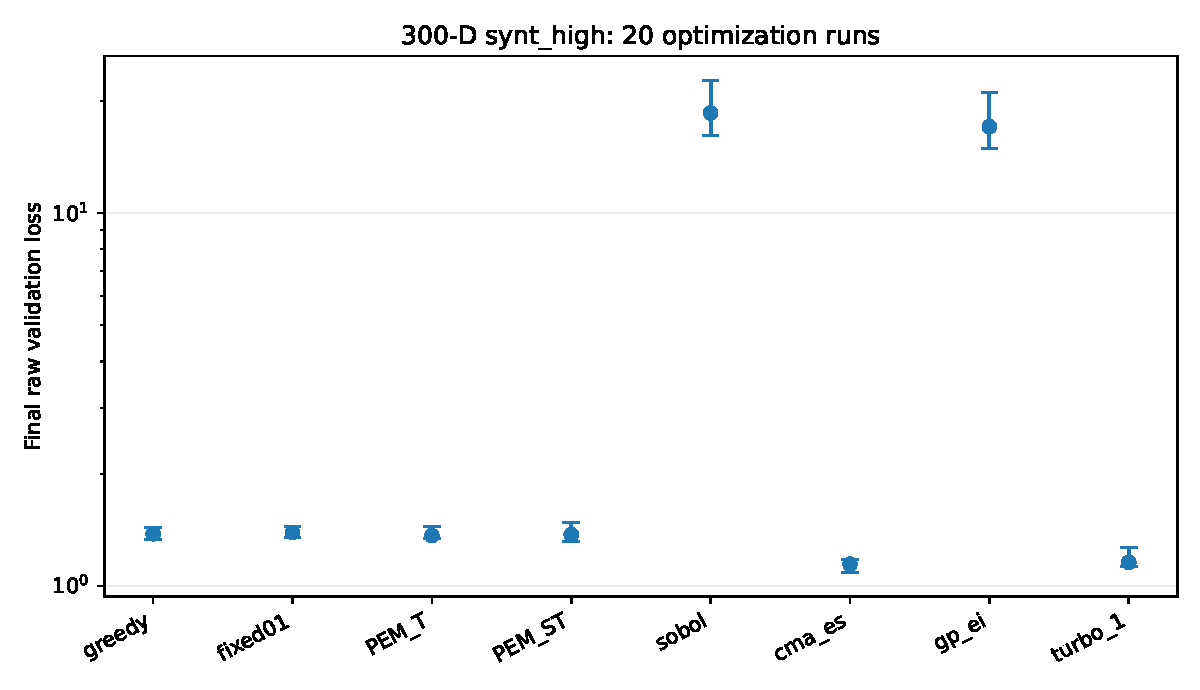
\includegraphics[width=\linewidth,height=.65\textheight,keepaspectratio]{figures/supp_figure_9.pdf}
\caption{Endpoints on 300-dimensional synt\_high, with 20 optimization runs per method. Points show median original validation loss and vertical bars span the 25th--75th percentiles. The vertical axis is logarithmic; lower is better.}
\end{figure}

Figure S9 separates the 300-dimensional methods into two endpoint groups. The four internal configurations, CMA-ES, and TuRBO-1 finish near the lower cluster, whereas Sobol and GP-EI remain more than an order of magnitude higher on the logarithmic axis. Interquartile bars are shown for all methods so that the apparent grouping can be assessed against between-run variability.

The associated paid-budget convergence histories are shown in Figure S10.

\begin{figure}[H]
\centering
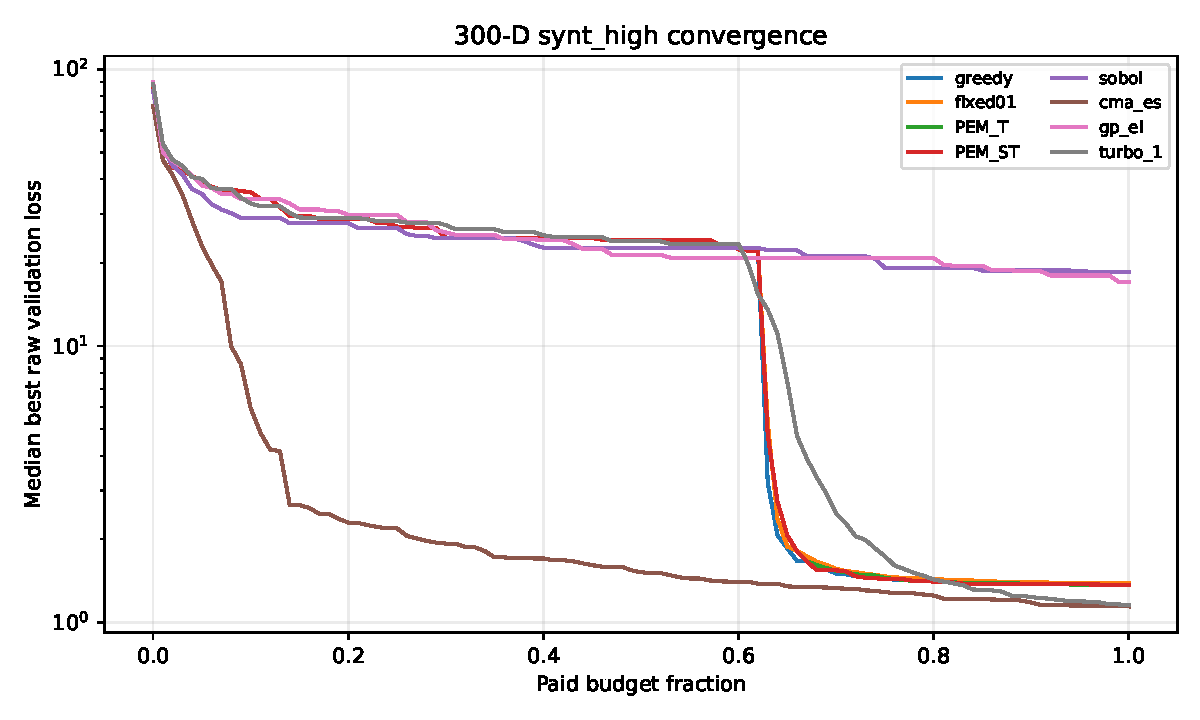
\includegraphics[width=\linewidth,height=.65\textheight,keepaspectratio]{figures/supp_figure_10.pdf}
\caption{Convergence on 300-dimensional synt\_high under 1,000 paid evaluations. Each line shows the median best original validation loss across 20 runs against paid-budget fraction. The vertical axis is logarithmic.}
\end{figure}

Figure S10 reveals distinct routes to the lower endpoint cluster. The brown CMA-ES curve falls substantially during the early budget, followed by gradual reductions. The four internal curves fall sharply after initialization consumes about 62\% of the budget. The grey TuRBO-1 curve also declines substantially after this fraction and approaches CMA-ES near the endpoint. Sobol and GP-EI remain in the higher-loss group. The 1,000-evaluation protocol is reported separately from the primary 500-evaluation application study.

The prespecified descriptive PEM\_\allowbreak T-minus-fixed 01 median raw-loss difference was -0.01788, with paired-run bootstrap interval {[}-0.06477, 0.05017{]} and 11/9/0 negative/positive/zero differences. No p-value was computed and this contrast was not added to the three-test primary application family. The interval conditions on one fixed data set and split.

\hypertarget{selected-point-feedback-and-resource-boundary}{%
\subsection{Selected-point feedback and resource boundary}\label{selected-point-feedback-and-resource-boundary}}

\FloatBarrier\begingroup\fontsize{8.5}{10.5}\selectfont\setlength\tabcolsep{3pt}

\begin{longtable}[]{@{}
  >{\raggedright\arraybackslash}p{(\columnwidth - 12\tabcolsep) * \real{0.1429}}
  >{\raggedleft\arraybackslash}p{(\columnwidth - 12\tabcolsep) * \real{0.1429}}
  >{\raggedleft\arraybackslash}p{(\columnwidth - 12\tabcolsep) * \real{0.1429}}
  >{\raggedleft\arraybackslash}p{(\columnwidth - 12\tabcolsep) * \real{0.1429}}
  >{\raggedleft\arraybackslash}p{(\columnwidth - 12\tabcolsep) * \real{0.1429}}
  >{\raggedleft\arraybackslash}p{(\columnwidth - 12\tabcolsep) * \real{0.1429}}
  >{\raggedleft\arraybackslash}p{(\columnwidth - 12\tabcolsep) * \real{0.1429}}@{}}
\caption{Selected-point feedback and resource boundary.}\tabularnewline
\toprule\noalign{}
\begin{minipage}[b]{\linewidth}\raggedright
Method
\end{minipage} & \begin{minipage}[b]{\linewidth}\raggedleft
Failure
\end{minipage} & \begin{minipage}[b]{\linewidth}\raggedleft
QLoss
\end{minipage} & \begin{minipage}[b]{\linewidth}\raggedleft
Explore
\end{minipage} & \begin{minipage}[b]{\linewidth}\raggedleft
Fallback
\end{minipage} & \begin{minipage}[b]{\linewidth}\raggedleft
Claims
\end{minipage} & \begin{minipage}[b]{\linewidth}\raggedleft
FDP
\end{minipage} \\
\midrule\noalign{}
\endfirsthead
\toprule\noalign{}
\begin{minipage}[b]{\linewidth}\raggedright
Method
\end{minipage} & \begin{minipage}[b]{\linewidth}\raggedleft
Failure
\end{minipage} & \begin{minipage}[b]{\linewidth}\raggedleft
QLoss
\end{minipage} & \begin{minipage}[b]{\linewidth}\raggedleft
Explore
\end{minipage} & \begin{minipage}[b]{\linewidth}\raggedleft
Fallback
\end{minipage} & \begin{minipage}[b]{\linewidth}\raggedleft
Claims
\end{minipage} & \begin{minipage}[b]{\linewidth}\raggedleft
FDP
\end{minipage} \\
\midrule\noalign{}
\endhead
\bottomrule\noalign{}
\endlastfoot
greedy & 0.07447 & 0.01695 & 0 & 0 & 257 & 1 \\
fixed01 & 0.07895 & 0.03878 & 0.09618 & 0 & 127 & 0.9921 \\
PEM\_\allowbreak T & 0.08921 & 0.07535 & 0.3405 & 0 & 5 & 1 \\
PEM\_\allowbreak ST & 0.1266 & 0.06124 & 0.3854 & 0.01184 & 119 & 0.9916 \\
\end{longtable}

\endgroup

Feedback summaries cover the 380 post-initialization selections per internal run. They describe each closed-loop history and do not establish same-pool causal effects or conformal error control. Before formal labels, eight separate full-budget resource runs completed 8,000 validation evaluations and zero test calls. Their mixed-load timings supported feasibility only; formal optimization times are reported as observed process costs rather than exclusive speedups.

\hypertarget{prespecified-model-and-training-cap-sensitivity}{%
\section{Prespecified model and training-cap sensitivity}\label{prespecified-model-and-training-cap-sensitivity}}

Five preselected BBOB structure representatives (f1, f6, f10, f15, f20), dimensions 20/40, instances 14--16, and three optimization repeats evaluated PEM\_\allowbreak T under the base setting and four one-factor perturbations. All 450 runs and 135,000 paid evaluations completed; no hidden diagnostic labels or inferential tests were added. This local sensitivity study does not select a replacement default.

\FloatBarrier\begingroup\fontsize{8.5}{10.5}\selectfont\setlength\tabcolsep{3pt}

\begin{longtable}[]{@{}
  >{\raggedleft\arraybackslash}p{(\columnwidth - 6\tabcolsep) * \real{0.2500}}
  >{\raggedright\arraybackslash}p{(\columnwidth - 6\tabcolsep) * \real{0.2500}}
  >{\raggedright\arraybackslash}p{(\columnwidth - 6\tabcolsep) * \real{0.2500}}
  >{\raggedright\arraybackslash}p{(\columnwidth - 6\tabcolsep) * \real{0.2500}}@{}}
\caption{Prespecified model and training-cap sensitivity.}\tabularnewline
\toprule\noalign{}
\begin{minipage}[b]{\linewidth}\raggedleft
D
\end{minipage} & \begin{minipage}[b]{\linewidth}\raggedright
Variant
\end{minipage} & \begin{minipage}[b]{\linewidth}\raggedright
Endpoint median {[}Q1, Q3{]}
\end{minipage} & \begin{minipage}[b]{\linewidth}\raggedright
AUC median {[}Q1, Q3{]}
\end{minipage} \\
\midrule\noalign{}
\endfirsthead
\toprule\noalign{}
\begin{minipage}[b]{\linewidth}\raggedleft
D
\end{minipage} & \begin{minipage}[b]{\linewidth}\raggedright
Variant
\end{minipage} & \begin{minipage}[b]{\linewidth}\raggedright
Endpoint median {[}Q1, Q3{]}
\end{minipage} & \begin{minipage}[b]{\linewidth}\raggedright
AUC median {[}Q1, Q3{]}
\end{minipage} \\
\midrule\noalign{}
\endhead
\bottomrule\noalign{}
\endlastfoot
20 & base & -1.536 {[}-2.168, -0.8568{]} & -0.962 {[}-1.292, -0.5037{]} \\
20 & cap128 & -1.439 {[}-1.903, -0.7494{]} & -0.9267 {[}-1.28, -0.5181{]} \\
20 & cap512 & -1.536 {[}-2.168, -0.8568{]} & -0.962 {[}-1.292, -0.5037{]} \\
20 & scale125 & -1.085 {[}-1.722, -0.6441{]} & -0.6593 {[}-1.087, -0.3838{]} \\
20 & scale500 & -1.473 {[}-2.095, -0.6943{]} & -0.776 {[}-1.079, -0.4353{]} \\
40 & base & -1.275 {[}-1.676, -0.8544{]} & -0.8335 {[}-1.096, -0.5196{]} \\
40 & cap128 & -0.9176 {[}-1.179, -0.5716{]} & -0.6855 {[}-0.8808, -0.4435{]} \\
40 & cap512 & -1.235 {[}-1.69, -0.8008{]} & -0.8185 {[}-1.123, -0.5374{]} \\
40 & scale125 & -0.8456 {[}-1.18, -0.5364{]} & -0.5406 {[}-0.7806, -0.3901{]} \\
40 & scale500 & -1.151 {[}-1.311, -0.7564{]} & -0.7301 {[}-0.9111, -0.4361{]} \\
\end{longtable}

\endgroup

Paired model and training-cap endpoint distributions are shown in Figure S11.

\begin{figure}[H]
\centering
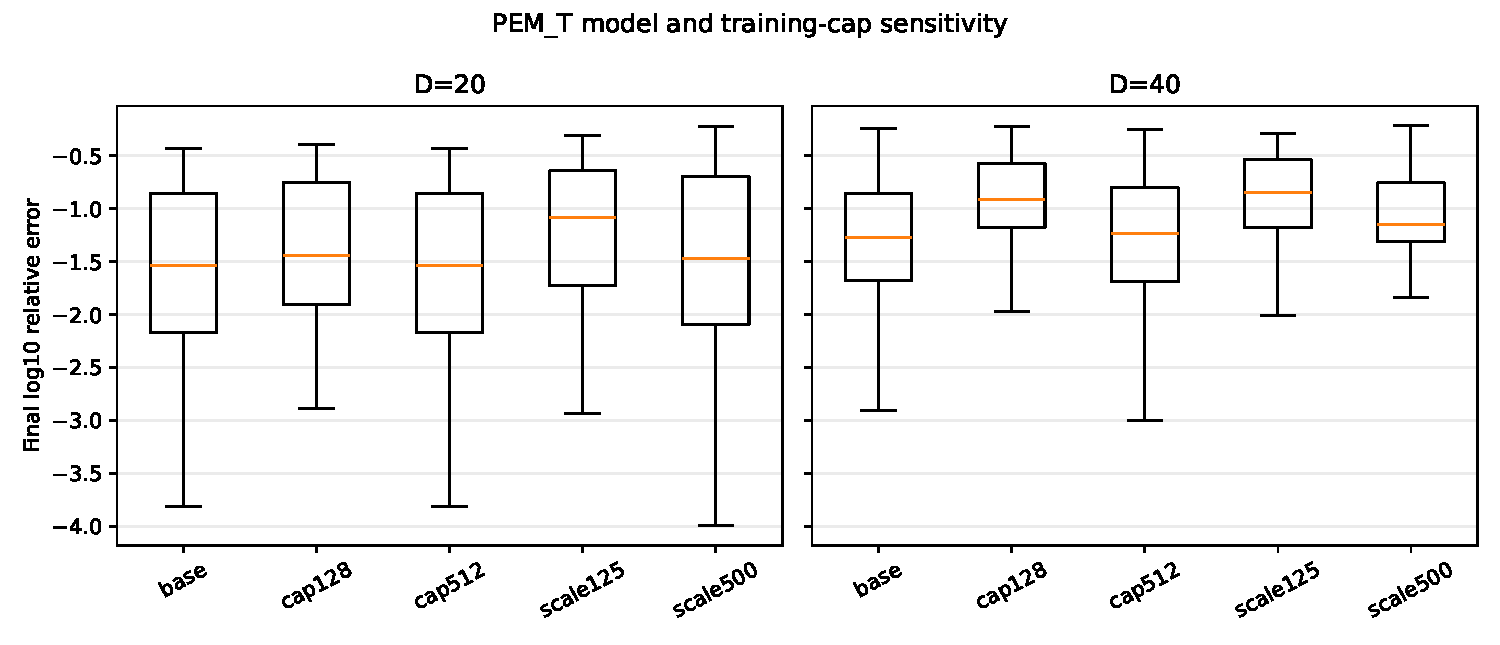
\includegraphics[width=\linewidth,height=.65\textheight,keepaspectratio]{figures/supp_figure_11.pdf}
\caption{Final $\log_{10}$ relative-error distributions for model and training-cap variants in dimensions 20 and 40. Boxes span the interquartile range and central lines show medians. Whiskers extend to the most extreme observations within 1.5 interquartile ranges of the box; outlier points are omitted. Lower is better.}
\end{figure}

Figure S11 compares the base model, training caps of 128 and 512, and length-scale variants 1.25 and 5.00 on the same sensitivity cases. Cap512 coincides with the base configuration in dimension 20 because the cap is never reached. The scale125 boxes have higher medians than the base boxes in both dimensions, indicating worse final error under that variant. Changes in medians and interquartile ranges are reported separately from the paired variant-minus-base differences below.

Paired differences below are variant minus base in final log10 relative error. Negative values favor the variant descriptively.

\FloatBarrier\begingroup\fontsize{8.5}{10.5}\selectfont\setlength\tabcolsep{3pt}

\begin{longtable}[]{@{}
  >{\raggedleft\arraybackslash}p{(\columnwidth - 10\tabcolsep) * \real{0.1667}}
  >{\raggedright\arraybackslash}p{(\columnwidth - 10\tabcolsep) * \real{0.1667}}
  >{\raggedright\arraybackslash}p{(\columnwidth - 10\tabcolsep) * \real{0.1667}}
  >{\raggedleft\arraybackslash}p{(\columnwidth - 10\tabcolsep) * \real{0.1667}}
  >{\raggedleft\arraybackslash}p{(\columnwidth - 10\tabcolsep) * \real{0.1667}}
  >{\raggedleft\arraybackslash}p{(\columnwidth - 10\tabcolsep) * \real{0.1667}}@{}}
\caption{Prespecified model and training-cap sensitivity.}\tabularnewline
\toprule\noalign{}
\begin{minipage}[b]{\linewidth}\raggedleft
D
\end{minipage} & \begin{minipage}[b]{\linewidth}\raggedright
Variant
\end{minipage} & \begin{minipage}[b]{\linewidth}\raggedright
Difference median {[}Q1, Q3{]}
\end{minipage} & \begin{minipage}[b]{\linewidth}\raggedleft
Negative
\end{minipage} & \begin{minipage}[b]{\linewidth}\raggedleft
Positive
\end{minipage} & \begin{minipage}[b]{\linewidth}\raggedleft
Zero
\end{minipage} \\
\midrule\noalign{}
\endfirsthead
\toprule\noalign{}
\begin{minipage}[b]{\linewidth}\raggedleft
D
\end{minipage} & \begin{minipage}[b]{\linewidth}\raggedright
Variant
\end{minipage} & \begin{minipage}[b]{\linewidth}\raggedright
Difference median {[}Q1, Q3{]}
\end{minipage} & \begin{minipage}[b]{\linewidth}\raggedleft
Negative
\end{minipage} & \begin{minipage}[b]{\linewidth}\raggedleft
Positive
\end{minipage} & \begin{minipage}[b]{\linewidth}\raggedleft
Zero
\end{minipage} \\
\midrule\noalign{}
\endhead
\bottomrule\noalign{}
\endlastfoot
20 & cap128 & 0.06854 {[}0, 0.1836{]} & 11 & 30 & 4 \\
20 & cap512 & 0 {[}0, 0{]} & 0 & 0 & 45 \\
20 & scale125 & 0.2805 {[}0.08773, 0.5608{]} & 8 & 37 & 0 \\
20 & scale500 & 0.09344 {[}-0.04563, 0.2851{]} & 14 & 31 & 0 \\
40 & cap128 & 0.3284 {[}0.0957, 0.4718{]} & 4 & 41 & 0 \\
40 & cap512 & 0.005203 {[}-0.02706, 0.08161{]} & 18 & 27 & 0 \\
40 & scale125 & 0.3253 {[}0.03915, 0.656{]} & 8 & 37 & 0 \\
40 & scale500 & 0.09029 {[}-0.002699, 0.2816{]} & 12 & 33 & 0 \\
\end{longtable}

\endgroup

The 45 D=20 base/cap512 pairs had identical PRE/LABEL trajectories and candidate arrays, as neither cap was reached. Thus that equality is an implementation invariant rather than evidence that caps never matter. At D=40, cap512 is untruncated only within this 400-evaluation scope.

\FloatBarrier\begingroup\fontsize{8.5}{10.5}\selectfont\setlength\tabcolsep{3pt}

\begin{longtable}[]{@{}
  >{\raggedleft\arraybackslash}p{(\columnwidth - 10\tabcolsep) * \real{0.1667}}
  >{\raggedright\arraybackslash}p{(\columnwidth - 10\tabcolsep) * \real{0.1667}}
  >{\raggedleft\arraybackslash}p{(\columnwidth - 10\tabcolsep) * \real{0.1667}}
  >{\raggedleft\arraybackslash}p{(\columnwidth - 10\tabcolsep) * \real{0.1667}}
  >{\raggedleft\arraybackslash}p{(\columnwidth - 10\tabcolsep) * \real{0.1667}}
  >{\raggedleft\arraybackslash}p{(\columnwidth - 10\tabcolsep) * \real{0.1667}}@{}}
\caption{Prespecified model and training-cap sensitivity.}\tabularnewline
\toprule\noalign{}
\begin{minipage}[b]{\linewidth}\raggedleft
D
\end{minipage} & \begin{minipage}[b]{\linewidth}\raggedright
Variant
\end{minipage} & \begin{minipage}[b]{\linewidth}\raggedleft
Capped
\end{minipage} & \begin{minipage}[b]{\linewidth}\raggedleft
Failure
\end{minipage} & \begin{minipage}[b]{\linewidth}\raggedleft
Explore
\end{minipage} & \begin{minipage}[b]{\linewidth}\raggedleft
Fallback
\end{minipage} \\
\midrule\noalign{}
\endfirsthead
\toprule\noalign{}
\begin{minipage}[b]{\linewidth}\raggedleft
D
\end{minipage} & \begin{minipage}[b]{\linewidth}\raggedright
Variant
\end{minipage} & \begin{minipage}[b]{\linewidth}\raggedleft
Capped
\end{minipage} & \begin{minipage}[b]{\linewidth}\raggedleft
Failure
\end{minipage} & \begin{minipage}[b]{\linewidth}\raggedleft
Explore
\end{minipage} & \begin{minipage}[b]{\linewidth}\raggedleft
Fallback
\end{minipage} \\
\midrule\noalign{}
\endhead
\bottomrule\noalign{}
\endlastfoot
20 & base & 0 & 0.08746 & 0.2789 & 0 \\
20 & cap128 & 3195 & 0.1332 & 0.3444 & 0 \\
20 & cap512 & 0 & 0.08746 & 0.2789 & 0 \\
20 & scale125 & 0 & 0.1002 & 0.3173 & 0 \\
20 & scale500 & 0 & 0.07175 & 0.283 & 0 \\
40 & base & 6435 & 0.08889 & 0.2541 & 0 \\
40 & cap128 & 12195 & 0.1893 & 0.5487 & 0 \\
40 & cap512 & 0 & 0.08993 & 0.2591 & 0 \\
40 & scale125 & 6435 & 0.09733 & 0.2797 & 0 \\
40 & scale500 & 6435 & 0.08674 & 0.2902 & 0 \\
\end{longtable}

\endgroup

Feedback metrics follow each variant's distinct closed-loop history. The limited function/instance set, shared initialization, and absence of multiplicity-adjusted inference restrict these results to robustness description.

\hypertarget{prespecified-budget-performance-sensitivity-and-recovery-accounting}{%
\section{Prespecified budget-performance sensitivity and recovery accounting}\label{prespecified-budget-performance-sensitivity-and-recovery-accounting}}

\hypertarget{design-and-aggregation}{%
\subsection{Design and aggregation}\label{design-and-aggregation}}

Five prespecified BBOB structure representatives (f1, f6, f10, f15, and f20), dimensions 20/40, instances 17--19, and three repeats were run independently at total budgets 5D, 10D, and 15D. Six internal configurations and four external references completed all 2,700 runs and 810,000 paid evaluations, with no diagnostic labels. Each endpoint uses the matching fixed 01 common-initialization error as a post-run denominator. The repeat median is first taken within each function-instance cell; the three instances within each function and the five function scores are then averaged with equal weight. No hypothesis test, confidence interval, or parameter selection was added.

\hypertarget{endpoints-and-convergence-1}{%
\subsection{Endpoints and convergence}\label{endpoints-and-convergence-1}}

Lower values are better. Each table entry is the prespecified hierarchical mean final log10 relative error.

\FloatBarrier\begingroup\fontsize{8.5}{10.5}\selectfont\setlength\tabcolsep{3pt}

\begin{longtable}[]{@{}
  >{\raggedright\arraybackslash}p{(\columnwidth - 12\tabcolsep) * \real{0.1429}}
  >{\raggedleft\arraybackslash}p{(\columnwidth - 12\tabcolsep) * \real{0.1429}}
  >{\raggedleft\arraybackslash}p{(\columnwidth - 12\tabcolsep) * \real{0.1429}}
  >{\raggedleft\arraybackslash}p{(\columnwidth - 12\tabcolsep) * \real{0.1429}}
  >{\raggedleft\arraybackslash}p{(\columnwidth - 12\tabcolsep) * \real{0.1429}}
  >{\raggedleft\arraybackslash}p{(\columnwidth - 12\tabcolsep) * \real{0.1429}}
  >{\raggedleft\arraybackslash}p{(\columnwidth - 12\tabcolsep) * \real{0.1429}}@{}}
\caption{Endpoints and convergence.}\tabularnewline
\toprule\noalign{}
\begin{minipage}[b]{\linewidth}\raggedright
Method
\end{minipage} & \begin{minipage}[b]{\linewidth}\raggedleft
D20-5D
\end{minipage} & \begin{minipage}[b]{\linewidth}\raggedleft
D20-10D
\end{minipage} & \begin{minipage}[b]{\linewidth}\raggedleft
D20-15D
\end{minipage} & \begin{minipage}[b]{\linewidth}\raggedleft
D40-5D
\end{minipage} & \begin{minipage}[b]{\linewidth}\raggedleft
D40-10D
\end{minipage} & \begin{minipage}[b]{\linewidth}\raggedleft
D40-15D
\end{minipage} \\
\midrule\noalign{}
\endfirsthead
\toprule\noalign{}
\begin{minipage}[b]{\linewidth}\raggedright
Method
\end{minipage} & \begin{minipage}[b]{\linewidth}\raggedleft
D20-5D
\end{minipage} & \begin{minipage}[b]{\linewidth}\raggedleft
D20-10D
\end{minipage} & \begin{minipage}[b]{\linewidth}\raggedleft
D20-15D
\end{minipage} & \begin{minipage}[b]{\linewidth}\raggedleft
D40-5D
\end{minipage} & \begin{minipage}[b]{\linewidth}\raggedleft
D40-10D
\end{minipage} & \begin{minipage}[b]{\linewidth}\raggedleft
D40-15D
\end{minipage} \\
\midrule\noalign{}
\endhead
\bottomrule\noalign{}
\endlastfoot
greedy & -0.961 & -1.768 & -2.097 & -0.9999 & -1.544 & -1.643 \\
fixed01 & -0.9322 & -1.749 & -2.035 & -0.9727 & -1.53 & -1.664 \\
fixed03 & -0.6895 & -1.616 & -2.041 & -0.7998 & -1.491 & -1.634 \\
pool\_\allowbreak random & -0.08979 & -0.3369 & -0.433 & -0.187 & -0.3509 & -0.4963 \\
PEM\_\allowbreak T & -0.7538 & -1.689 & -1.987 & -0.8891 & -1.477 & -1.598 \\
PEM\_\allowbreak ST & -0.7407 & -1.676 & -2.039 & -0.8906 & -1.456 & -1.57 \\
sobol & -0.1024 & -0.1513 & -0.209 & -0.0429 & -0.09157 & -0.09792 \\
cma\_\allowbreak es & -0.4835 & -0.7414 & -1.068 & -0.4553 & -0.6883 & -0.949 \\
gp\_\allowbreak ei & -1.642 & -2.388 & -2.574 & -1.651 & -1.993 & -2.174 \\
turbo\_\allowbreak 1 & -1.08 & -2.216 & -2.502 & -0.9778 & -1.943 & -2.516 \\
\end{longtable}

\endgroup

Endpoint changes across the three prespecified total budgets are shown in Figure S12.

\begin{figure}[H]
\centering
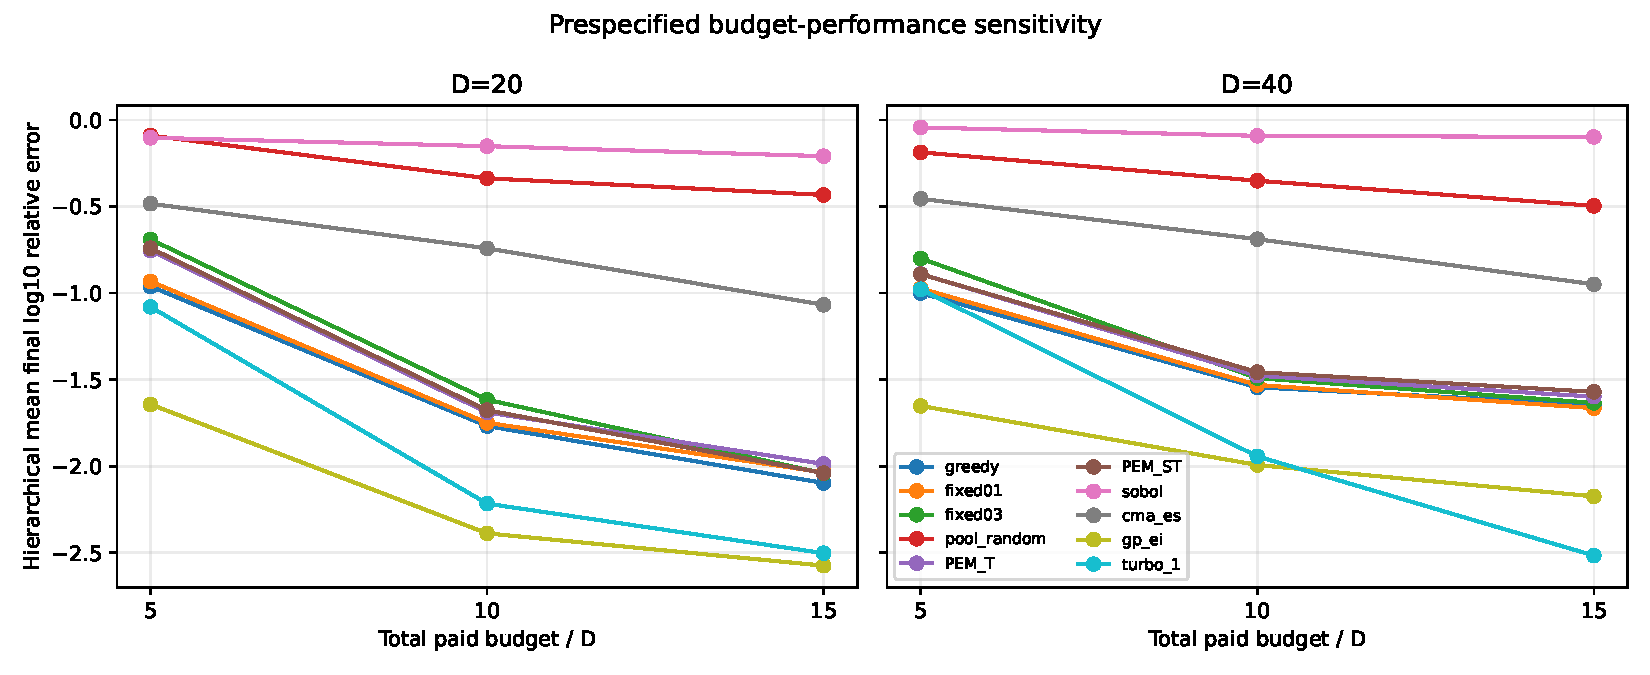
\includegraphics[width=\linewidth,height=.65\textheight,keepaspectratio]{figures/supp_figure_12.pdf}
\caption{Budget-sensitivity endpoints for dimensions 20 and 40. The horizontal axis is total paid budget divided by dimension, with values 5, 10 and 15. Markers show hierarchical mean final $\log_{10}$ relative error and lines connect the three recorded budgets for each method; lower is better.}
\end{figure}

Figure S12 connects endpoint quality to total budget in separate dimension-20 and dimension-40 panels. Hierarchical aggregation retains repeat medians within each function--instance cell before averaging across the problem set. Most curves descend as the allowance increases from $5D$ to $15D$; GP-EI and TuRBO-1 retain lower endpoints than the internal configurations. The connecting segments summarize the three tested budgets and do not interpolate unobserved runs.

The corresponding separately executed convergence histories are shown in Figure S13.

\begin{figure}[H]
\centering
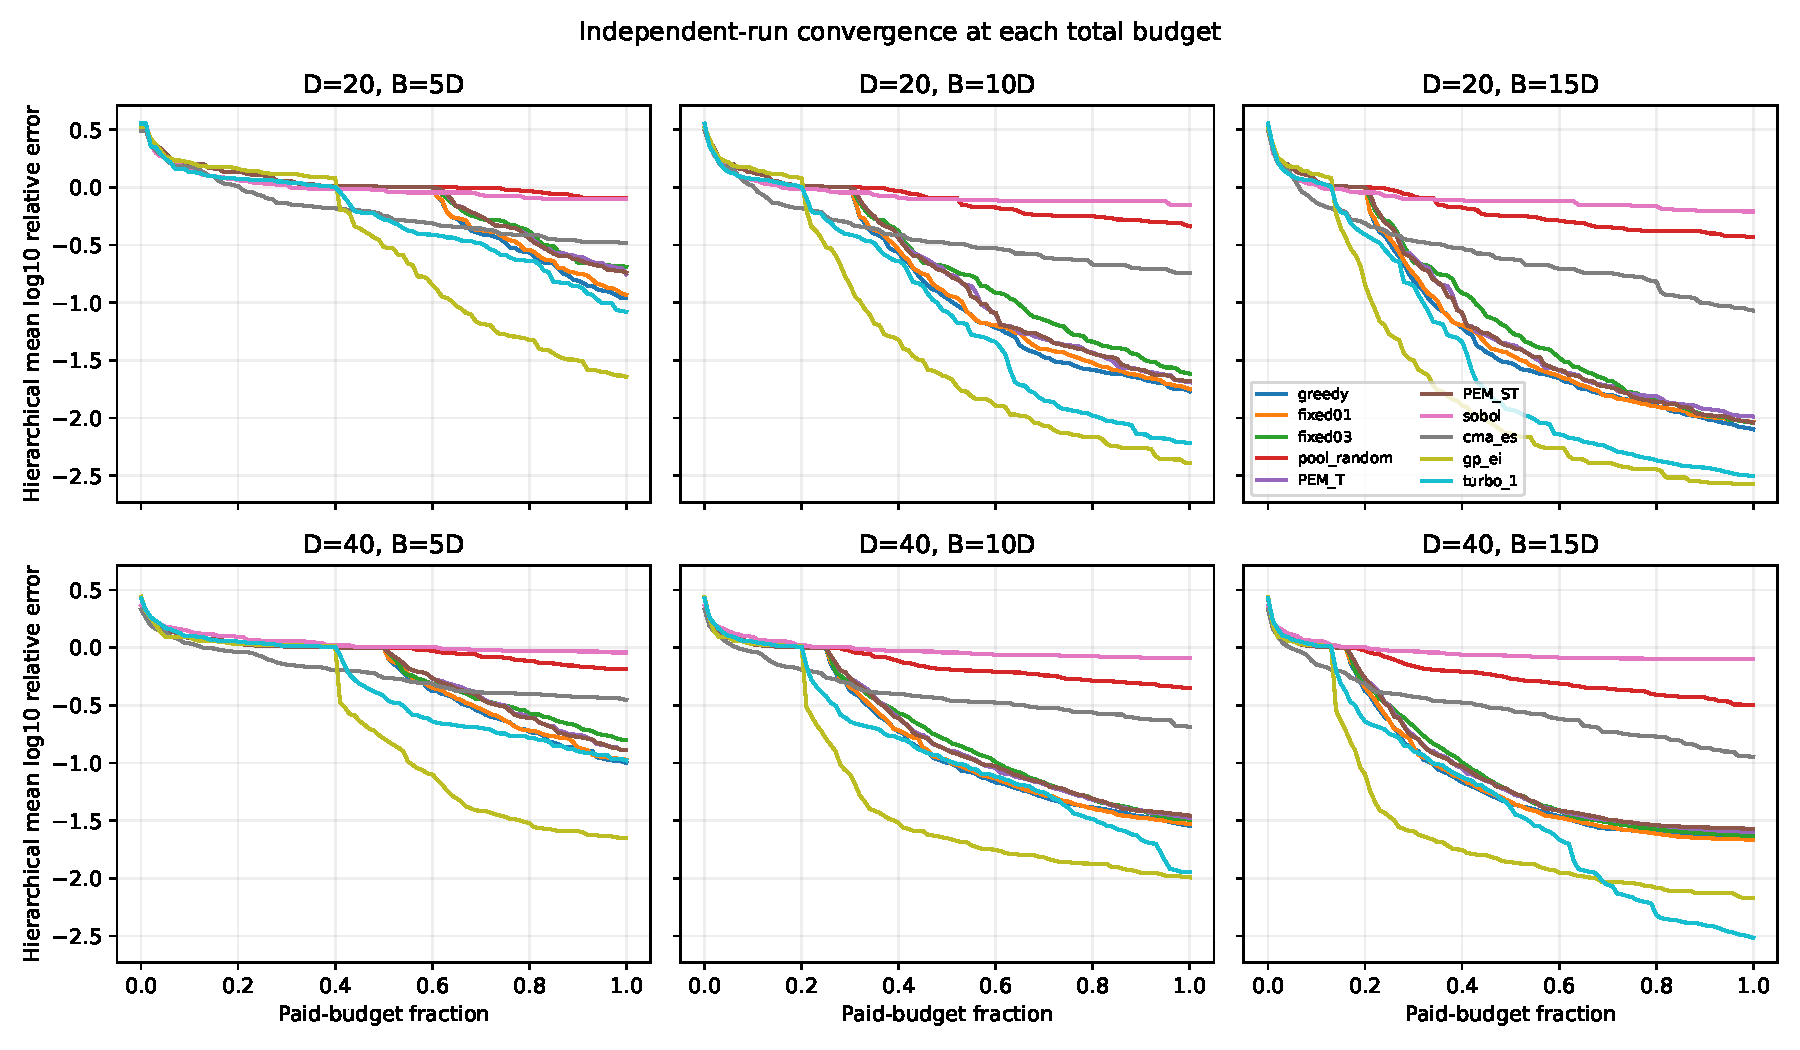
\includegraphics[width=\linewidth,height=.65\textheight,keepaspectratio]{figures/supp_figure_13.pdf}
\caption{Budget-sensitivity convergence, with $D=20$ in the upper row and $D=40$ in the lower row; columns use total budgets $5D$, $10D$ and $15D$. Each horizontal axis is the fraction of that panel's paid budget. Lines show hierarchical mean $\log_{10}$ relative error; lower is better.}
\end{figure}

Figure S13 plots separately executed runs against their own paid-budget fractions. The same absolute evaluation count occurs farther left as total budget increases across the columns. Matched internal information prefixes therefore occupy different horizontal fractions in the three budgets; the prefix audit compares absolute label order. External methods retain their own initialization and search histories. The six panels display convergence within each budget and dimension.

Each budget is a separate optimization run. A longer-budget endpoint therefore supplies robustness evidence under a larger total allowance; it is not a continuation selected after observing the shorter run. The restricted five-function, two-dimension design and descriptive aggregation do not establish a general ranking.

\hypertarget{prefix-and-information-order-audit}{%
\subsection{Prefix and information-order audit}\label{prefix-and-information-order-audit}}

\FloatBarrier\begingroup\fontsize{8.5}{10.5}\selectfont\setlength\tabcolsep{3pt}

\begin{longtable}[]{@{}
  >{\raggedright\arraybackslash}p{(\columnwidth - 4\tabcolsep) * \real{0.3333}}
  >{\raggedright\arraybackslash}p{(\columnwidth - 4\tabcolsep) * \real{0.3333}}
  >{\raggedright\arraybackslash}p{(\columnwidth - 4\tabcolsep) * \real{0.3333}}@{}}
\caption{Prefix and information-order audit.}\tabularnewline
\toprule\noalign{}
\begin{minipage}[b]{\linewidth}\raggedright
Method
\end{minipage} & \begin{minipage}[b]{\linewidth}\raggedright
Equal 5D/10D/15D prefixes
\end{minipage} & \begin{minipage}[b]{\linewidth}\raggedright
Required invariant
\end{minipage} \\
\midrule\noalign{}
\endfirsthead
\toprule\noalign{}
\begin{minipage}[b]{\linewidth}\raggedright
Method
\end{minipage} & \begin{minipage}[b]{\linewidth}\raggedright
Equal 5D/10D/15D prefixes
\end{minipage} & \begin{minipage}[b]{\linewidth}\raggedright
Required invariant
\end{minipage} \\
\midrule\noalign{}
\endhead
\bottomrule\noalign{}
\endlastfoot
greedy & 90/90 & yes \\
fixed01 & 90/90 & yes \\
fixed03 & 90/90 & yes \\
pool\_\allowbreak random & 90/90 & yes \\
PEM\_\allowbreak T & 90/90 & yes \\
PEM\_\allowbreak ST & 90/90 & yes \\
sobol & 90/90 & no \\
cma\_\allowbreak es & 90/90 & no \\
gp\_\allowbreak ei & 0/90 & no \\
turbo\_\allowbreak 1 & 0/90 & no \\
\end{longtable}

\endgroup

The budget-blind internal core was required to reproduce identical 5D and 10D prefixes inside the corresponding longer run; all 540 required comparisons passed. External prefix equality was recorded rather than required: 180/360 comparisons were equal. That count is an implementation observation, not an assumption used to validate external methods. Full audits replayed all 810,000 PRE/LABEL pairs, internal bounds and management states, and 7,020 raw-file hashes. No total-budget value entered the internal proposal rule.

\hypertarget{recovery-accounting-and-evidence-boundary}{%
\subsection{Recovery accounting and evidence boundary}\label{recovery-accounting-and-evidence-boundary}}

The budget-sensitivity interruption left 8 incomplete units with 1,791 physically acquired labels. Their complete directories were archived before resumption, and each affected unit was rerun from its frozen seed. These labels never entered the 2,700 canonical trajectories. The budget-sensitivity physical ledger is therefore 811,791 calls: 810,000 canonical evaluations plus 1,791 disclosed interrupted-run calls. The additional calls are excluded from endpoints, convergence curves, and algorithm budgets.

The completed GP-EI performance batch contains 151,200 canonical algorithm evaluations. During interruption recovery, one GP-EI point (evaluation 349 of gp\_\allowbreak ei\_\allowbreak f02\_\allowbreak d40\_\allowbreak i13\_\allowbreak r2\_\allowbreak b400) was physically queried a second time because the newer partial journal contained 348 labels while an earlier archive contained 349. The point and returned label matched exactly; the label entered the optimizer history once, so the canonical 400-step trajectory and endpoint are unchanged. The physical GP-EI ledger is therefore 151,201 calls: 151,200 canonical evaluations plus one disclosed recovery-validation call. The extra call is excluded from algorithm budgets, performance curves, and exclusive-cost analysis. The read-only recovery audit made zero objective calls and verified eight recovered trajectories (2,800 canonical evaluations), 2,014 saved second-generation labels, and 786 second-generation physical calls, one of which overlaps the earlier archive.

The original development-benefit gate failed. The archived study therefore reports decision-consequence auditing results. A CEC batch started on 24 September 2026 was stopped after the scope decision; its 30 complete and 8 partial trajectories are retained as exploratory records and excluded from manuscript statistics. A verifiable author-code DRSO comparison is provided in S8.2; the three originally named but unavailable implementations continue to delimit method-specific claims.

\hypertarget{reproducibility-inventory}{%
\section{Reproducibility inventory}\label{reproducibility-inventory}}

The archived evidence contains frozen protocols, source hashes, dependency locks, deterministic seed maps, prediction-before-label journals, candidate arrays, separate diagnostic labels, endpoint re-evaluations, raw-file hashes, analysis tables, and figure sources. Diagnostic labels never enter optimizer histories. Interrupted or repeated physical calls are disclosed separately from canonical algorithm budgets. The repository contains sources and curated revision evidence. The byte-preserving GP source bundle, frozen intervention records and lossless compact transfer release support the added results. Larger historical archives remain available from the corresponding author upon reasonable request. Frozen source revisions, data-release commits and file checksums identify the evidence.

\hypertarget{finite-element-audit}{%
\subsection{Finite-element audit}\label{finite-element-audit}}

The EngiBench beam batch contains 50 complete runs, 10,000 canonical finite-element evaluations, 50 independent endpoint re-evaluations, zero failures, and maximum volume-fraction error 1.665e-16. The audit verifies the complete design, source hashes, 100 raw-file hashes, prediction-before-label ordering, exact endpoint replay, and separation of the earlier smoke run from method selection.

\hypertarget{matched-initialization-external-reference-acquisition-and-saea-sensitivity}{%
\subsection{Matched-initialization external-reference, acquisition, and SAEA sensitivity}\label{matched-initialization-external-reference-acquisition-and-saea-sensitivity}}

The supplemental beam experiment gives GP-EI and TuRBO-1 exactly the same 58-point initial finite-element archive used by Greedy, fixed 01, and PEM-T in each repeat. It contains 20 complete trajectories and 4,000 algorithm-budget observations: 1,160 previously paid deterministic initial labels and 2,840 additional finite-element calls. The event-level audit finds zero failures, zero exact duplicate points, complete prediction-before-label order, and exact agreement with all ten source-archive hashes. Forty additional physical calls belong only to two independent endpoint-diagnostic rounds and never enter an optimizer history. The accepted diagnostic table has maximum absolute difference 1.50e-8 and maximum relative difference 6.23e-12.

\FloatBarrier\begingroup\fontsize{8.5}{10.5}\selectfont\setlength\tabcolsep{3pt}

\begin{longtable}[]{@{}
  >{\raggedright\arraybackslash}p{(\columnwidth - 14\tabcolsep) * \real{0.1250}}
  >{\raggedleft\arraybackslash}p{(\columnwidth - 14\tabcolsep) * \real{0.1250}}
  >{\raggedleft\arraybackslash}p{(\columnwidth - 14\tabcolsep) * \real{0.1250}}
  >{\raggedleft\arraybackslash}p{(\columnwidth - 14\tabcolsep) * \real{0.1250}}
  >{\raggedleft\arraybackslash}p{(\columnwidth - 14\tabcolsep) * \real{0.1250}}
  >{\raggedleft\arraybackslash}p{(\columnwidth - 14\tabcolsep) * \real{0.1250}}
  >{\raggedleft\arraybackslash}p{(\columnwidth - 14\tabcolsep) * \real{0.1250}}
  >{\raggedleft\arraybackslash}p{(\columnwidth - 14\tabcolsep) * \real{0.1250}}@{}}
\caption{Matched-initialization external-reference, acquisition, and SAEA sensitivity.}\tabularnewline
\toprule\noalign{}
\begin{minipage}[b]{\linewidth}\raggedright
Method
\end{minipage} & \begin{minipage}[b]{\linewidth}\raggedleft
Shared-init median
\end{minipage} & \begin{minipage}[b]{\linewidth}\raggedleft
Native-init median
\end{minipage} & \begin{minipage}[b]{\linewidth}\raggedleft
Median shared-minus-native
\end{minipage} & \begin{minipage}[b]{\linewidth}\raggedleft
Holm p
\end{minipage} & \begin{minipage}[b]{\linewidth}\raggedleft
Median shared-minus-PEM-T
\end{minipage} & \begin{minipage}[b]{\linewidth}\raggedleft
Wins/\allowbreak ties/\allowbreak losses vs PEM-T
\end{minipage} & \begin{minipage}[b]{\linewidth}\raggedleft
Holm p
\end{minipage} \\
\midrule\noalign{}
\endfirsthead
\toprule\noalign{}
\begin{minipage}[b]{\linewidth}\raggedright
Method
\end{minipage} & \begin{minipage}[b]{\linewidth}\raggedleft
Shared-init median
\end{minipage} & \begin{minipage}[b]{\linewidth}\raggedleft
Native-init median
\end{minipage} & \begin{minipage}[b]{\linewidth}\raggedleft
Median shared-minus-native
\end{minipage} & \begin{minipage}[b]{\linewidth}\raggedleft
Holm p
\end{minipage} & \begin{minipage}[b]{\linewidth}\raggedleft
Median shared-minus-PEM-T
\end{minipage} & \begin{minipage}[b]{\linewidth}\raggedleft
Wins/\allowbreak ties/\allowbreak losses vs PEM-T
\end{minipage} & \begin{minipage}[b]{\linewidth}\raggedleft
Holm p
\end{minipage} \\
\midrule\noalign{}
\endhead
\bottomrule\noalign{}
\endlastfoot
GP-EI & 2308.5 & 2117.5 & +399.8 & 0.320 & +242.8 & 1/3/6 & 0.0469 \\
TuRBO-1 & 574.0 & 578.2 & -44.7 & 0.695 & -1372.3 & 10/0/0 & 0.00391 \\
\end{longtable}

\endgroup

The initial launch stopped after a missing fixed-seed argument prevented two GP-EI workers from entering GP search; those logs contain only reused initial labels and zero subsequent objective calls. Six already-running TuRBO-1 units completed through an unaffected branch. The complete launch state was archived, the one-argument wiring error was corrected, and the remaining units resumed. The terminal audit accepts six original and fourteen corrected code hashes after verifying that the change lies outside the completed TuRBO branch. No failed or interrupted GP label enters the 20 canonical trajectories.

Two further Gaussian-process acquisition controls use the same ten 58-point archives, 200-evaluation budget, Matérn-5/2 model, 4,096-point Sobol candidate pool, and eight local optimization starts. GP-PI uses an improvement margin equal to 0.01 times the current response standard deviation. GP-UCB is implemented for minimization by selecting the lowest value of mean minus 2.0 standard deviations. These 20 trajectories contain 4,000 algorithm-budget observations, including 1,160 reused labels and 2,840 new finite-element calls. The audit verifies sequential prediction-before-label records, bounds, finite outputs, exact source-archive hashes, complete budgets, and zero exact duplicate points.

\begingroup\renewcommand\thetable{S25a}

\FloatBarrier\begingroup\fontsize{8.5}{10.5}\selectfont\setlength\tabcolsep{3pt}

\begin{longtable}[]{@{}
  >{\raggedright\arraybackslash}p{(\columnwidth - 14\tabcolsep) * \real{0.1250}}
  >{\raggedleft\arraybackslash}p{(\columnwidth - 14\tabcolsep) * \real{0.1250}}
  >{\raggedleft\arraybackslash}p{(\columnwidth - 14\tabcolsep) * \real{0.1250}}
  >{\raggedleft\arraybackslash}p{(\columnwidth - 14\tabcolsep) * \real{0.1250}}
  >{\raggedleft\arraybackslash}p{(\columnwidth - 14\tabcolsep) * \real{0.1250}}
  >{\raggedleft\arraybackslash}p{(\columnwidth - 14\tabcolsep) * \real{0.1250}}
  >{\raggedleft\arraybackslash}p{(\columnwidth - 14\tabcolsep) * \real{0.1250}}
  >{\raggedleft\arraybackslash}p{(\columnwidth - 14\tabcolsep) * \real{0.1250}}@{}}
\caption{Additional shared-initialization acquisition and relation-model controls.}\tabularnewline
\toprule\noalign{}
\begin{minipage}[b]{\linewidth}\raggedright
Method
\end{minipage} & \begin{minipage}[b]{\linewidth}\raggedleft
Shared-init median
\end{minipage} & \begin{minipage}[b]{\linewidth}\raggedleft
Q1
\end{minipage} & \begin{minipage}[b]{\linewidth}\raggedleft
Q3
\end{minipage} & \begin{minipage}[b]{\linewidth}\raggedleft
Median improvement after initialization
\end{minipage} & \begin{minipage}[b]{\linewidth}\raggedleft
Median difference vs PEM-T
\end{minipage} & \begin{minipage}[b]{\linewidth}\raggedleft
Wins/\allowbreak ties/\allowbreak losses vs PEM-T
\end{minipage} & \begin{minipage}[b]{\linewidth}\raggedleft
Holm p
\end{minipage} \\
\midrule\noalign{}
\endfirsthead
\toprule\noalign{}
\begin{minipage}[b]{\linewidth}\raggedright
Method
\end{minipage} & \begin{minipage}[b]{\linewidth}\raggedleft
Shared-init median
\end{minipage} & \begin{minipage}[b]{\linewidth}\raggedleft
Q1
\end{minipage} & \begin{minipage}[b]{\linewidth}\raggedleft
Q3
\end{minipage} & \begin{minipage}[b]{\linewidth}\raggedleft
Median improvement after initialization
\end{minipage} & \begin{minipage}[b]{\linewidth}\raggedleft
Median difference vs PEM-T
\end{minipage} & \begin{minipage}[b]{\linewidth}\raggedleft
Wins/\allowbreak ties/\allowbreak losses vs PEM-T
\end{minipage} & \begin{minipage}[b]{\linewidth}\raggedleft
Holm p
\end{minipage} \\
\midrule\noalign{}
\endhead
\bottomrule\noalign{}
\endlastfoot
GP-PI & 1233.1 & 921.2 & 1399.7 & 0.517 & -876.1 & 9/0/1 & 0.0117 \\
GP-UCB & 2308.7 & 2223.8 & 2827.3 & 0.000 & +574.6 & 2/2/6 & 0.0391 \\
DRSO & 647.4 & 580.4 & 780.0 & 0.747 & -1334.6 & 9/0/1 & 0.0117 \\
\end{longtable}

\endgroup

\addtocounter{table}{-1}\endgroup

The different outcomes under a common surrogate and common starting archive isolate acquisition behavior. Candidate-dependent uncertainty is structurally capable of changing decisions, but its practical value depends on how uncertainty and predicted objective value are combined. GP-PI supplies a successful candidate-dependent control; the fixed-multiplier GP-UCB control does not improve the median initial incumbent under this budget. The three rows form one Holm family.

DRSO supplies a competitive surrogate-assisted evolutionary comparison. The public author repository is frozen at commit \texttt{03c19d4280b38230e0852054922072f5aa6dcdf5} under LGPL-3.0. Its relation models, unevaluated-population mechanism, reproduction, training cap of 100, and other algorithm settings remain unchanged. Population size is set from the author default of 50 to 58 only because the common archive contains 58 points. A Python 3.12 compatibility namespace supplies the removed \texttt{imp} name required by pyDOE2 and an unused optional callback import; neither compatibility file alters the DRSO search implementation.

The DRSO batch contains ten complete trajectories and 2,000 algorithm-budget observations: 580 reused initial labels and 1,420 new finite-element calls. All 4,010 event records have sequential PRE/LABEL order, all ten source-archive and author-tree hashes match, and no trajectory contains an out-of-bounds, nonfinite, or exact duplicate point. The author-code result object, external paid-call journal, and endpoint minimum agree in every repeat. DRSO improves median compliance by 74.7\% after initialization and reaches 647.4, compared with 1972.8 for PEM-T.

\hypertarget{evidence-boundary}{%
\subsection{Evidence boundary}\label{evidence-boundary}}

The empirical residual monitor has no claimed pointwise coverage theorem, false-discovery-rate guarantee, regret bound, or global convergence theorem. Broad BBOB comparisons with external methods retain native initialization and remain descriptive; the beam sensitivity alone supplies a matched initial archive. GP-PI and GP-UCB are transparent acquisition controls, while DRSO is an author-code published SAEA. The 19-dimensional beam family does not establish performance for unrestricted 5,000-variable topology optimization. Full CEC exploration was stopped after the decision-consequence auditing scope was selected; its exploratory trajectories are excluded from all article statistics. Temporal CP-SAEA, SADE-SS, and BGP-SAEA remain excluded because matching executable author implementations with frozen versions, parameters, and licenses were unavailable; similarly named public implementations are not substituted for them. The DRSO comparison retains its author-code specification.

\hypertarget{frozen-gp-intervention-and-immediate-diagnostic-accounting}{%
\section{Frozen GP intervention and immediate diagnostic accounting}\label{frozen-gp-intervention-and-immediate-diagnostic-accounting}}

This additional study is separately frozen, descriptive, and not part of the original Holm families. Input hashes and 120 decisions were committed at f1c9bbdebc35071bd935d0b11c92857f5e07201e before new intervention labels. The initially transmitted binary ZIP was incomplete, despite an intact local author-supplied archive. Local scientific input hashes and frozen choices did not change. The public input release now uses a byte-preserving text bundle at commit 71e074945262e1dbfc223726c7216e5415385ddc, replacing the incomplete repository binary. Its restoration checks every original file hash, all segment hashes and the decoded payload hash before writing any file. It preserves all 60 original file bytes, including line endings; it does not claim to reconstruct the original ZIP container bytes. The original supplied archive remains identified by SHA256 c59079aaf34f560ee2f3e93a55bd60e13b2fa4c53097285842580df4d3b8098b. Public distribution integrity and scientific execution integrity are separate checks.

Thirty source histories contain 6,000 budgeted algorithm observations and 580 distinct common initial labels across ten repeats. Frozen states stop at PRE(t), exclude LABEL(t), and contain only observations before 59,101,151 or 200. The same recorded ARD Matérn-5/2 posterior scores mean, EI, PI and LCB on 4,096 scrambled Sobol points plus the original action. EI uses zero margin, PI uses 0.01 times the training standard deviation, and LCB uses kappa 2. Logged hyperparameters are not refitted. All120 source-action mean/standard-deviation comparisons satisfy rtol=atol=1e-8. Decisions and candidate records are hashed before source action labels are looked up. No new diagnostic label enters a source optimizer history.

\FloatBarrier\begingroup\fontsize{8.5}{10.5}\selectfont\setlength\tabcolsep{3pt}

\begin{longtable}[]{@{}
  >{\raggedright\arraybackslash}p{(\columnwidth - 8\tabcolsep) * \real{0.2000}}
  >{\raggedright\arraybackslash}p{(\columnwidth - 8\tabcolsep) * \real{0.2000}}
  >{\raggedright\arraybackslash}p{(\columnwidth - 8\tabcolsep) * \real{0.2000}}
  >{\raggedright\arraybackslash}p{(\columnwidth - 8\tabcolsep) * \real{0.2000}}
  >{\raggedright\arraybackslash}p{(\columnwidth - 8\tabcolsep) * \real{0.2000}}@{}}
\caption{All controls and source-history groups. Four checkpoint estimates are averaged within each repeat before averaging ten repeats. U and DeltaU are in units of 1e-6.}\tabularnewline
\toprule\noalign{}
\begin{minipage}[b]{\linewidth}\raggedright
Source history
\end{minipage} & \begin{minipage}[b]{\linewidth}\raggedright
Control
\end{minipage} & \begin{minipage}[b]{\linewidth}\raggedright
Changed (\%)
\end{minipage} & \begin{minipage}[b]{\linewidth}\raggedright
Mean U (1e-6)
\end{minipage} & \begin{minipage}[b]{\linewidth}\raggedright
DeltaU vs mean (1e-6)
\end{minipage} \\
\midrule\noalign{}
\endfirsthead
\toprule\noalign{}
\begin{minipage}[b]{\linewidth}\raggedright
Source history
\end{minipage} & \begin{minipage}[b]{\linewidth}\raggedright
Control
\end{minipage} & \begin{minipage}[b]{\linewidth}\raggedright
Changed (\%)
\end{minipage} & \begin{minipage}[b]{\linewidth}\raggedright
Mean U (1e-6)
\end{minipage} & \begin{minipage}[b]{\linewidth}\raggedright
DeltaU vs mean (1e-6)
\end{minipage} \\
\midrule\noalign{}
\endhead
\bottomrule\noalign{}
\endlastfoot
EI history & MEAN & 0.0 & 0.899669 & +0.000000 \\
EI history & EI & 30.0 & 0.899669 & +0.000000 \\
EI history & PI & 25.0 & 0.899669 & +0.000000 \\
EI history & LCB & 52.5 & 0.000000 & -0.899669 \\
PI history & MEAN & 0.0 & 0.347088 & +0.000000 \\
PI history & EI & 95.0 & 0.000000 & -0.347088 \\
PI history & PI & 7.5 & 0.347088 & +0.000000 \\
PI history & LCB & 97.5 & 0.000000 & -0.347088 \\
UCB history & MEAN & 0.0 & 0.877758 & +0.000000 \\
UCB history & EI & 30.0 & 0.887232 & +0.009475 \\
UCB history & PI & 35.0 & 1.178882 & +0.301124 \\
UCB history & LCB & 75.0 & 0.511893 & -0.365864 \\
\end{longtable}

\endgroup

The training scale ranges from 733152 to 9.12154e+08. This can make normalized gains small even when raw compliance changes. The metric is retained as frozen; no post hoc replacement or new p-value is used. These comparisons neither test delayed exploration nor authorize promotion.

The 480 control-state choices reduce to 261 distinct within-state actions. Source-action reuse accounts for 120 responses; exact diagnostic reuse across states accounts for 3;138 are new FE calls. New diagnostic FE time is 4.437432s and GP state preparation time13.435883s. The initial solver compatibility check made42 calls before detecting a 4.929e-8 relative discrepancy at a large-compliance point. That discrepancy was numerical, not a failed FE response. The complete retained60-call check uses the disclosed1e-6 relative tolerance and passes every comparison. The original prediction replay tolerance remains1e-8. The first42 outputs and timings were not retained but their attempts are included. The retained solver check takes 2.327726s. Total additional attempts for this GP revision are 240. These observed times do not establish exclusive wall-time savings.

\hypertarget{independent-load-position-transfer-horizon-effects-and-paid-workflows}{%
\section{Independent load-position transfer, horizon effects and paid workflows}\label{independent-load-position-transfer-horizon-effects-and-paid-workflows}}

The protocol and executable implementation were committed at 7555d58b145a2c44b73bab5ec47d0f643a57dde1 before acquiring new transfer labels. Conditions forcedist0.25 and 0.75 each have ten independently seeded58-point Sobol initializations. Fixed seed namespaces distinguish initialization, pilots and validation. The same case/step candidate namespace is shared across policies inside a phase. All policies use one shared specification; tie ordering, fit limits and budgets were not tuned using outcomes. This is within-family physical-condition transfer, not cross-domain validation.

\FloatBarrier\begingroup\fontsize{8.5}{10.5}\selectfont\setlength\tabcolsep{3pt}

\begin{longtable}[]{@{}
  >{\raggedright\arraybackslash}p{(\columnwidth - 4\tabcolsep) * \real{0.3333}}
  >{\raggedright\arraybackslash}p{(\columnwidth - 4\tabcolsep) * \real{0.3333}}
  >{\raggedright\arraybackslash}p{(\columnwidth - 4\tabcolsep) * \real{0.3333}}@{}}
\caption{Differences between the two additional GP experiments. The original beam wrapper, material, supports, volume 0.35 and dimension 19 are retained.}\tabularnewline
\toprule\noalign{}
\begin{minipage}[b]{\linewidth}\raggedright
Setting
\end{minipage} & \begin{minipage}[b]{\linewidth}\raggedright
Frozen intervention (S9)
\end{minipage} & \begin{minipage}[b]{\linewidth}\raggedright
Independent transfer (S10)
\end{minipage} \\
\midrule\noalign{}
\endfirsthead
\toprule\noalign{}
\begin{minipage}[b]{\linewidth}\raggedright
Setting
\end{minipage} & \begin{minipage}[b]{\linewidth}\raggedright
Frozen intervention (S9)
\end{minipage} & \begin{minipage}[b]{\linewidth}\raggedright
Independent transfer (S10)
\end{minipage} \\
\midrule\noalign{}
\endhead
\bottomrule\noalign{}
\endlastfoot
Source state & Archived EI/PI/UCB histories & Fresh initialization in each force condition \\
Kernel & Logged ARD Matérn-5/2 & Isotropic Matérn-5/2 \\
Hyperparameters & Frozen, optimizer disabled & L-BFGS-B, max100 iterations, no restarts \\
Candidate pool & 4096 Sobol + original action & 1024 Sobol; observed points excluded \\
EI margin & 0 & 0.01 times training standard deviation \\
PI margin / LCB kappa & 0.01 scaled / 2 & 0.01 scaled / 2 \\
GP alpha / normalization & 1e-6 / normalized targets & 1e-6 / normalized targets \\
Physical force position & 0.0 & 0.25 and 0.75 \\
\end{longtable}

\endgroup

The transfer constant bounds are{[}0.05,20{]} and length-scale bounds{[}0.005,2{]}, with initial length scale 0.2. Fit convergence warnings are recorded and do not trigger restarts. Beams2D caches force-dependent matrices; each case creates a fresh problem object configured once with its actual force position. This prevents cross-condition state reuse. The environment pins NumPy 2.2.6, SciPy 1.15.3, scikit-learn1.7.2, EngiBench 0.2.0 and cvxopt1.3.2. These settings define a separate controlled study and do not rerun the historical ARD/continuous-refinement GP optimizer.

\hypertarget{paid-selection-and-independent-validation}{%
\subsection{Paid selection and independent validation}\label{paid-selection-and-independent-validation}}

Each audited workflow pays 58 initial labels,4x20 pilot labels and 142 selected-policy validation labels:280. Each complete portfolio independently pays 58 initial labels and 4x142 continuation labels:626. A fixed single policy needs200. The pilot winner is the lowest final pilot compliance, with exact ties broken in PI, mean, EI, LCB order. Selection is persisted after 138 calls and before any canonical validation label. Canonical histories start again from the initial58 labels and never include pilot responses. Validation candidates use a different namespace; no warm-starting selector is claimed. The selected canonical trajectory and its separately paid portfolio counterpart agree exactly in every repeat. All duplicate designs across workflows are physically evaluated and counted, rather than credited as free labels.

\FloatBarrier\begingroup\fontsize{8.5}{10.5}\selectfont\setlength\tabcolsep{3pt}

\begin{longtable}[]{@{}
  >{\raggedright\arraybackslash}p{(\columnwidth - 14\tabcolsep) * \real{0.1250}}
  >{\raggedright\arraybackslash}p{(\columnwidth - 14\tabcolsep) * \real{0.1250}}
  >{\raggedright\arraybackslash}p{(\columnwidth - 14\tabcolsep) * \real{0.1250}}
  >{\raggedright\arraybackslash}p{(\columnwidth - 14\tabcolsep) * \real{0.1250}}
  >{\raggedright\arraybackslash}p{(\columnwidth - 14\tabcolsep) * \real{0.1250}}
  >{\raggedright\arraybackslash}p{(\columnwidth - 14\tabcolsep) * \real{0.1250}}
  >{\raggedright\arraybackslash}p{(\columnwidth - 14\tabcolsep) * \real{0.1250}}
  >{\raggedright\arraybackslash}p{(\columnwidth - 14\tabcolsep) * \real{0.1250}}@{}}
\caption{All twenty paired endpoints. The selected-policy column is the prespecified independent canonical endpoint. All-paid best is a secondary descriptive endpoint including every pilot design; it does not replace the validation criterion. Gap is 100x(selected/portfolio-best-1).}\tabularnewline
\toprule\noalign{}
\begin{minipage}[b]{\linewidth}\raggedright
Force
\end{minipage} & \begin{minipage}[b]{\linewidth}\raggedright
Rep
\end{minipage} & \begin{minipage}[b]{\linewidth}\raggedright
Selected
\end{minipage} & \begin{minipage}[b]{\linewidth}\raggedright
Initial
\end{minipage} & \begin{minipage}[b]{\linewidth}\raggedright
Selected-policy
\end{minipage} & \begin{minipage}[b]{\linewidth}\raggedright
Portfolio-best
\end{minipage} & \begin{minipage}[b]{\linewidth}\raggedright
Gap (\%)
\end{minipage} & \begin{minipage}[b]{\linewidth}\raggedright
All-paid best
\end{minipage} \\
\midrule\noalign{}
\endfirsthead
\toprule\noalign{}
\begin{minipage}[b]{\linewidth}\raggedright
Force
\end{minipage} & \begin{minipage}[b]{\linewidth}\raggedright
Rep
\end{minipage} & \begin{minipage}[b]{\linewidth}\raggedright
Selected
\end{minipage} & \begin{minipage}[b]{\linewidth}\raggedright
Initial
\end{minipage} & \begin{minipage}[b]{\linewidth}\raggedright
Selected-policy
\end{minipage} & \begin{minipage}[b]{\linewidth}\raggedright
Portfolio-best
\end{minipage} & \begin{minipage}[b]{\linewidth}\raggedright
Gap (\%)
\end{minipage} & \begin{minipage}[b]{\linewidth}\raggedright
All-paid best
\end{minipage} \\
\midrule\noalign{}
\endhead
\bottomrule\noalign{}
\endlastfoot
0.25 & 0 & PI & 1559.326 & 1350.207 & 1350.207 & 0.000 & 1350.207 \\
0.25 & 1 & EI & 1657.740 & 1192.164 & 805.832 & 47.942 & 1192.164 \\
0.25 & 2 & PI & 1817.963 & 929.539 & 929.539 & 0.000 & 929.539 \\
0.25 & 3 & EI & 3373.312 & 1048.640 & 923.095 & 13.600 & 1048.640 \\
0.25 & 4 & PI & 1392.373 & 1152.823 & 1015.625 & 13.509 & 1152.823 \\
0.25 & 5 & PI & 1426.446 & 1426.446 & 1195.130 & 19.355 & 1426.446 \\
0.25 & 6 & PI & 2081.842 & 956.490 & 915.138 & 4.519 & 956.490 \\
0.25 & 7 & MEAN & 1458.044 & 1204.446 & 1204.446 & 0.000 & 1065.517 \\
0.25 & 8 & PI & 1189.521 & 956.887 & 956.887 & 0.000 & 956.887 \\
0.25 & 9 & MEAN & 1774.608 & 1535.851 & 838.957 & 83.067 & 1392.803 \\
0.75 & 0 & PI & 1287.356 & 430.374 & 430.374 & 0.000 & 430.374 \\
0.75 & 1 & PI & 779.191 & 303.745 & 303.745 & 0.000 & 303.745 \\
0.75 & 2 & LCB & 653.215 & 454.896 & 315.137 & 44.349 & 375.564 \\
0.75 & 3 & PI & 703.816 & 326.950 & 326.950 & 0.000 & 326.950 \\
0.75 & 4 & MEAN & 607.672 & 481.780 & 351.951 & 36.889 & 327.563 \\
0.75 & 5 & PI & 644.397 & 335.272 & 332.477 & 0.841 & 312.168 \\
0.75 & 6 & PI & 697.634 & 383.191 & 325.992 & 17.546 & 383.191 \\
0.75 & 7 & PI & 997.734 & 677.303 & 174.014 & 289.223 & 597.821 \\
0.75 & 8 & PI & 583.133 & 429.673 & 274.350 & 56.615 & 285.959 \\
0.75 & 9 & PI & 720.317 & 303.082 & 211.908 & 43.025 & 253.360 \\
\end{longtable}

\endgroup

The primary median paired gaps are 9.013698\% and 27.217435\%. Exact portfolio-best matches are 4/10 and 3/10. The selected counts are PI6, EI2, mean2 at force 0.25, and PI8, LCB1, mean1 at force 0.75. Exact pilot-end ties occur in 7 and 4 repeats; counts should not be interpreted independently of the tie rule. The secondary all-paid gaps have medians9.013698\% and 2.115716\%. The discrepancy between primary and secondary endpoints is disclosed because the practical availability of a pilot design differs from evidence that the chosen policy transfers well.

\FloatBarrier\begingroup\fontsize{8.5}{10.5}\selectfont\setlength\tabcolsep{3pt}

\begin{longtable}[]{@{}
  >{\raggedright\arraybackslash}p{(\columnwidth - 8\tabcolsep) * \real{0.2000}}
  >{\raggedright\arraybackslash}p{(\columnwidth - 8\tabcolsep) * \real{0.2000}}
  >{\raggedright\arraybackslash}p{(\columnwidth - 8\tabcolsep) * \real{0.2000}}
  >{\raggedright\arraybackslash}p{(\columnwidth - 8\tabcolsep) * \real{0.2000}}
  >{\raggedright\arraybackslash}p{(\columnwidth - 8\tabcolsep) * \real{0.2000}}@{}}
\caption{Each200-call fixed policy compared with the280-call selected workflow. Median effects are paired100x(selected/fixed-1); negative favors selection. Wins/\allowbreak ties/\allowbreak losses are descriptive, not tests of superiority or equivalence.}\tabularnewline
\toprule\noalign{}
\begin{minipage}[b]{\linewidth}\raggedright
Force
\end{minipage} & \begin{minipage}[b]{\linewidth}\raggedright
Fixed policy
\end{minipage} & \begin{minipage}[b]{\linewidth}\raggedright
Median fixed compliance
\end{minipage} & \begin{minipage}[b]{\linewidth}\raggedright
Paired effect (\%)
\end{minipage} & \begin{minipage}[b]{\linewidth}\raggedright
Selection wins/ties/losses
\end{minipage} \\
\midrule\noalign{}
\endfirsthead
\toprule\noalign{}
\begin{minipage}[b]{\linewidth}\raggedright
Force
\end{minipage} & \begin{minipage}[b]{\linewidth}\raggedright
Fixed policy
\end{minipage} & \begin{minipage}[b]{\linewidth}\raggedright
Median fixed compliance
\end{minipage} & \begin{minipage}[b]{\linewidth}\raggedright
Paired effect (\%)
\end{minipage} & \begin{minipage}[b]{\linewidth}\raggedright
Selection wins/ties/losses
\end{minipage} \\
\midrule\noalign{}
\endhead
\bottomrule\noalign{}
\endlastfoot
0.25 & MEAN & 1102.310 & +0.000 & 4/2/4 \\
0.25 & EI & 1233.521 & -1.813 & 5/3/2 \\
0.25 & PI & 956.689 & +0.000 & 1/6/3 \\
0.25 & LCB & 1360.425 & -8.978 & 7/1/2 \\
0.75 & MEAN & 326.834 & +0.420 & 3/2/5 \\
0.75 & EI & 379.451 & -5.682 & 5/1/4 \\
0.75 & PI & 359.232 & +0.000 & 1/8/1 \\
0.75 & LCB & 475.896 & -6.764 & 5/3/2 \\
\end{longtable}

\endgroup

Selecting the best fixed policy retrospectively from these validation outcomes would be a separate selection procedure. No such200-call oracle advantage is attributed to the audit or its comparator.

\hypertarget{horizon-separation}{%
\subsection{Horizon separation}\label{horizon-separation}}

\FloatBarrier\begingroup\fontsize{8.5}{10.5}\selectfont\setlength\tabcolsep{3pt}

\begin{longtable}[]{@{}
  >{\raggedright\arraybackslash}p{(\columnwidth - 8\tabcolsep) * \real{0.2000}}
  >{\raggedright\arraybackslash}p{(\columnwidth - 8\tabcolsep) * \real{0.2000}}
  >{\raggedright\arraybackslash}p{(\columnwidth - 8\tabcolsep) * \real{0.2000}}
  >{\raggedright\arraybackslash}p{(\columnwidth - 8\tabcolsep) * \real{0.2000}}
  >{\raggedright\arraybackslash}p{(\columnwidth - 8\tabcolsep) * \real{0.2000}}@{}}
\caption{Pilot improvement from the common initial incumbent. First and 20-step columns are medians of per-repeat percentages. The final count concerns the same pilot trajectory.}\tabularnewline
\toprule\noalign{}
\begin{minipage}[b]{\linewidth}\raggedright
Force
\end{minipage} & \begin{minipage}[b]{\linewidth}\raggedright
Policy
\end{minipage} & \begin{minipage}[b]{\linewidth}\raggedright
First step (\%)
\end{minipage} & \begin{minipage}[b]{\linewidth}\raggedright
20 steps (\%)
\end{minipage} & \begin{minipage}[b]{\linewidth}\raggedright
Zero first, positive20 /10
\end{minipage} \\
\midrule\noalign{}
\endfirsthead
\toprule\noalign{}
\begin{minipage}[b]{\linewidth}\raggedright
Force
\end{minipage} & \begin{minipage}[b]{\linewidth}\raggedright
Policy
\end{minipage} & \begin{minipage}[b]{\linewidth}\raggedright
First step (\%)
\end{minipage} & \begin{minipage}[b]{\linewidth}\raggedright
20 steps (\%)
\end{minipage} & \begin{minipage}[b]{\linewidth}\raggedright
Zero first, positive20 /10
\end{minipage} \\
\midrule\noalign{}
\endhead
\bottomrule\noalign{}
\endlastfoot
0.25 & MEAN & 0.000 & 13.006 & 6 \\
0.25 & EI & 0.000 & 9.706 & 4 \\
0.25 & PI & 0.000 & 8.592 & 5 \\
0.25 & LCB & 0.000 & 2.514 & 4 \\
0.75 & MEAN & 0.000 & 42.350 & 8 \\
0.75 & EI & 0.000 & 13.491 & 5 \\
0.75 & PI & 0.000 & 46.765 & 7 \\
0.75 & LCB & 0.000 & 3.649 & 4 \\
\end{longtable}

\endgroup

\begin{figure}[H]
\centering
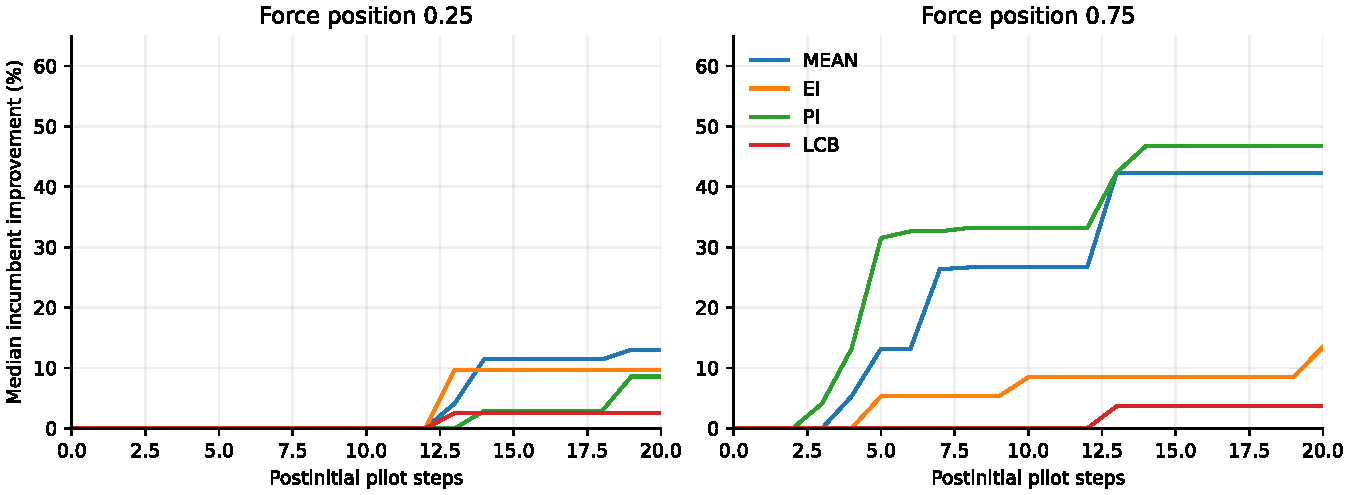
\includegraphics[width=\linewidth,height=.65\textheight,keepaspectratio]{figures/transfer_pilot_horizons.pdf}
\caption{Pilot incumbent improvement at force positions 0.25 (left) and 0.75 (right). The horizontal axis counts twenty postinitial pilot steps; the vertical axis is median percentage improvement from the initial incumbent. Blue, orange, green and red curves denote MEAN, EI, PI and LCB, respectively.}
\end{figure}

Figure S14 shows different timing across the two force positions. The force-position-0.25 curves have a long initial plateau before gains appear, whereas PI gains emerge earlier at force position 0.75. Later pilot gains can therefore follow an unchanged incumbent at the first step. These are whole-policy trajectories with diverging histories, so their differences do not estimate a first-action effect under an identical continuation. The canonical workflow uses a separate candidate stream.

\hypertarget{costs-recovery-and-evidence-integrity}{%
\subsection{Costs, recovery and evidence integrity}\label{costs-recovery-and-evidence-integrity}}

\FloatBarrier\begingroup\fontsize{8.5}{10.5}\selectfont\setlength\tabcolsep{3pt}

\begin{longtable}[]{@{}
  >{\raggedright\arraybackslash}p{(\columnwidth - 4\tabcolsep) * \real{0.3333}}
  >{\raggedright\arraybackslash}p{(\columnwidth - 4\tabcolsep) * \real{0.3333}}
  >{\raggedright\arraybackslash}p{(\columnwidth - 4\tabcolsep) * \real{0.3333}}@{}}
\caption{Additional FE-attempt boundary of the earlier GP/transfer stages. Later released checks are accounted for separately in Table~\ref{tab:extension_cost}; historical experiments before this revision are not included.}\tabularnewline
\toprule\noalign{}
\begin{minipage}[b]{\linewidth}\raggedright
Component
\end{minipage} & \begin{minipage}[b]{\linewidth}\raggedright
Physical attempts
\end{minipage} & \begin{minipage}[b]{\linewidth}\raggedright
Use in reported endpoints
\end{minipage} \\
\midrule\noalign{}
\endfirsthead
\toprule\noalign{}
\begin{minipage}[b]{\linewidth}\raggedright
Component
\end{minipage} & \begin{minipage}[b]{\linewidth}\raggedright
Physical attempts
\end{minipage} & \begin{minipage}[b]{\linewidth}\raggedright
Use in reported endpoints
\end{minipage} \\
\midrule\noalign{}
\endhead
\bottomrule\noalign{}
\endlastfoot
New frozen GP intervention & 138 & Separate diagnostics only \\
Solver compatibility verification & 102 & Never optimizer training \\
Earlier complete transfer execution & 18120 & Prior checked endpoints; raw journals unavailable in current workspace \\
Retained unchanged-protocol transfer recovery & 18120 & Retained canonical and pilot records, labels used once \\
Total including recovery & 36480 & No repeated attempt is hidden in a budget200 trajectory \\
\end{longtable}

\endgroup

The prior transfer journals became unavailable in the working environment before their raw release. An explicit recovery record at 62560a245a8b804dcff3ce00aa45aae0af9f3884 preserves the unchanged scientific configuration and caps additional recovery calls at 18,120. All twenty previously recorded selected-policy and portfolio-best endpoints are reproduced. Recovery contributes additional physical cost, not additional independent repeats or a changed inferential family. The initial zero-call bootstrap failure from the earlier launch adds no FE cost. The retained20 cases comprise2,320 physical initialization calls,1,600 pilot calls and 14,200 canonical postinitial calls. Their 100 full-budget trajectories contain 20,000 algorithm observations because initialization is shared among forks inside each workflow.

\FloatBarrier\begingroup\fontsize{8.5}{10.5}\selectfont\setlength\tabcolsep{3pt}

\begin{longtable}[]{@{}
  >{\raggedright\arraybackslash}p{(\columnwidth - 8\tabcolsep) * \real{0.2000}}
  >{\raggedright\arraybackslash}p{(\columnwidth - 8\tabcolsep) * \real{0.2000}}
  >{\raggedright\arraybackslash}p{(\columnwidth - 8\tabcolsep) * \real{0.2000}}
  >{\raggedright\arraybackslash}p{(\columnwidth - 8\tabcolsep) * \real{0.2000}}
  >{\raggedright\arraybackslash}p{(\columnwidth - 8\tabcolsep) * \real{0.2000}}@{}}
\caption{Retained observed component times summed across ten repeats per condition, in seconds. Four workers run concurrently; sums are not exclusive elapsed-time benchmarks.}\tabularnewline
\toprule\noalign{}
\begin{minipage}[b]{\linewidth}\raggedright
Force
\end{minipage} & \begin{minipage}[b]{\linewidth}\raggedright
Audited FE
\end{minipage} & \begin{minipage}[b]{\linewidth}\raggedright
Portfolio FE
\end{minipage} & \begin{minipage}[b]{\linewidth}\raggedright
Audited GP/selection
\end{minipage} & \begin{minipage}[b]{\linewidth}\raggedright
Portfolio GP/selection
\end{minipage} \\
\midrule\noalign{}
\endfirsthead
\toprule\noalign{}
\begin{minipage}[b]{\linewidth}\raggedright
Force
\end{minipage} & \begin{minipage}[b]{\linewidth}\raggedright
Audited FE
\end{minipage} & \begin{minipage}[b]{\linewidth}\raggedright
Portfolio FE
\end{minipage} & \begin{minipage}[b]{\linewidth}\raggedright
Audited GP/selection
\end{minipage} & \begin{minipage}[b]{\linewidth}\raggedright
Portfolio GP/selection
\end{minipage} \\
\midrule\noalign{}
\endhead
\bottomrule\noalign{}
\endlastfoot
0.25 & 90.395 & 194.651 & 57.242 & 175.964 \\
0.75 & 87.050 & 190.999 & 53.674 & 171.385 \\
\end{longtable}

\endgroup

The analyzer validates complete PRE/LABEL pairing,906 physical calls per case,280/626 workflow counts,20 pilot steps and 142 canonical steps per policy, selection before validation, correct seed namespaces, identical initial history hashes, exclusion of pilot labels from every canonical history, exact selected/portfolio trajectory replay, and every endpoint and component-time sum. It makes zero new FE calls. The compact release regenerates deterministic Sobol points and reconstructs each retained source JSONL byte for byte, checked against its SHA256; no objective call is needed to restore or analyze the records. Original full journals remain the source of timing and information-boundary checks.

The two load conditions evaluate within-family transfer with the fixed engineering parameterization. Their descriptive outcomes and component timings are reported under the frozen selection and validation protocols.

\FloatBarrier\begingroup\fontsize{8.5}{10.5}\selectfont\setlength\tabcolsep{3pt}
\begin{longtable}{@{}>{\raggedright\arraybackslash}p{(\columnwidth - 6\tabcolsep) * \real{0.19}}>{\raggedright\arraybackslash}p{(\columnwidth - 6\tabcolsep) * \real{0.39}}>{\raggedright\arraybackslash}p{(\columnwidth - 6\tabcolsep) * \real{0.17}}>{\raggedright\arraybackslash}p{(\columnwidth - 6\tabcolsep) * \real{0.25}}@{}}
\caption{Settings of separate evidence releases. The settings belong to separate implementations. All new GP records use alpha 1e-6 and normalized targets.}\label{tab:extension_settings}\tabularnewline
\toprule
Record & GP fitting & Candidate pool & Target \\
\midrule
\endfirsthead
\toprule
Record & GP fitting & Candidate pool & Target \\
\midrule
\endhead
\bottomrule
\endlastfoot
Original GP audit & Logged ARD Matérn-5/2; snapshot does not reoptimize & 4096 plus source action & 120 states; immediate alternatives \\
Common continuation & Same source ARD theta; fixed during branch updates & First: original pool; followup 1024 & 30 archived states; h0/1/3/5; mean continuation \\
Beam transfer & Isotropic Matérn-5/2; bounded L-BFGS-B, max 100 iterations per fit & 1024 & 20 fresh cases; full-policy pilots/continuations \\
Independent budget & ARD theta fitted once at shared 50-label warm state, max 30 iterations; then fixed & 1024; 8 calibration probes & 10 new seeds; 100-label states; mean/EI followup 5 \\
Thermal verification & Isotropic Matérn-5/2; fixed length 0.4; no hyperparameter fitting & 256 & 12 variables; 24 initial labels; 96 calls/workflow \\
\end{longtable}
\endgroup

\FloatBarrier\begingroup\fontsize{8.5}{10.5}\selectfont\setlength\tabcolsep{3pt}
\begin{longtable}{@{}>{\raggedright\arraybackslash}p{(\columnwidth - 2\tabcolsep) * \real{0.77}}>{\raggedright\arraybackslash}p{(\columnwidth - 2\tabcolsep) * \real{0.23}}@{}}
\caption{Archived common-continuation denominators. Original 90-contrast reporting is retained; action equivalence supplies a supplementary denominator over the same observations.}\label{tab:extension_denominators}\tabularnewline
\toprule
Reporting object & Count \\
\midrule
\endfirsthead
\toprule
Reporting object & Count \\
\midrule
\endhead
\bottomrule
\endlastfoot
Original named contrasts & 90 \\
Baseline-action aliases & 34 \\
Different-action named contrasts & 56 \\
Distinct nonbaseline-action contrasts & 46 \\
Named h0/h5 changes & 8 \\
Distinct-action changes & 7 \\
Distinct delayed non-ties & 6 \\
States containing changes & 4 \\
\end{longtable}
\endgroup

\FloatBarrier\begingroup\fontsize{8.5}{10.5}\selectfont\setlength\tabcolsep{3pt}
\begin{longtable}{@{}>{\raggedright\arraybackslash}p{(\columnwidth - 8\tabcolsep) * \real{0.21}}>{\raggedright\arraybackslash}p{(\columnwidth - 8\tabcolsep) * \real{0.14}}>{\raggedright\arraybackslash}p{(\columnwidth - 8\tabcolsep) * \real{0.21}}>{\raggedright\arraybackslash}p{(\columnwidth - 8\tabcolsep) * \real{0.21}}>{\raggedright\arraybackslash}p{(\columnwidth - 8\tabcolsep) * \real{0.23}}@{}}
\caption{Archived first-action contrasts with common posterior-mean continuation. Better/tie/worse counts use the original named-control denominator; each row has 10 dependent-source states and margin 1e-6. Positive advantage favours the named control.}\label{tab:extension_common}\tabularnewline
\toprule
Source history & Control & h0 B/T/W & h5 B/T/W & Median h5 (\%) \\
\midrule
\endfirsthead
\toprule
Source history & Control & h0 B/T/W & h5 B/T/W & Median h5 (\%) \\
\midrule
\endhead
\bottomrule
\endlastfoot
EI & EI & 0/10/0 & 1/9/0 & 0.000 \\
EI & PI & 0/10/0 & 1/8/1 & 0.000 \\
EI & LCB & 0/10/0 & 1/9/0 & 0.000 \\
PI & EI & 0/10/0 & 0/10/0 & 0.000 \\
PI & PI & 0/10/0 & 0/10/0 & 0.000 \\
PI & LCB & 0/10/0 & 0/10/0 & 0.000 \\
UCB & EI & 1/7/2 & 0/7/3 & 0.000 \\
UCB & PI & 0/9/1 & 0/8/2 & 0.000 \\
UCB & LCB & 0/8/2 & 1/6/3 & 0.000 \\
\end{longtable}
\endgroup

\FloatBarrier\begingroup\fontsize{8.5}{10.5}\selectfont\setlength\tabcolsep{3pt}
\begin{longtable}{@{}>{\raggedright\arraybackslash}p{(\columnwidth - 12\tabcolsep) * \real{0.12}}>{\raggedright\arraybackslash}p{(\columnwidth - 12\tabcolsep) * \real{0.1}}>{\raggedright\arraybackslash}p{(\columnwidth - 12\tabcolsep) * \real{0.2}}>{\raggedright\arraybackslash}p{(\columnwidth - 12\tabcolsep) * \real{0.13}}>{\raggedright\arraybackslash}p{(\columnwidth - 12\tabcolsep) * \real{0.1}}>{\raggedright\arraybackslash}p{(\columnwidth - 12\tabcolsep) * \real{0.13}}>{\raggedright\arraybackslash}p{(\columnwidth - 12\tabcolsep) * \real{0.22}}@{}}
\caption{Independent budget replay: horizon 5, margin 0.001,25 distinct nonbaseline-action contrasts per continuation. Requests are conservatively charged response lookups across 30 states. Calibration uses the stated root-EI proxy gate. Completed-horizon errors are computed after measuring the target.}\label{tab:extension_budget}\tabularnewline
\toprule
Followup & Budget & Rule & Classified & Errors & Requests & Selection regret (\%) \\
\midrule
\endfirsthead
\toprule
Followup & Budget & Rule & Classified & Errors & Requests & Selection regret (\%) \\
\midrule
\endhead
\bottomrule
\endlastfoot
MEAN & 12 & fixed depth & 17/25 & 0 & 204 & 0.0000 \\
MEAN & 12 & adaptive & 9/25 & 0 & 204 & 0.0000 \\
MEAN & 18 & calibration & 6/25 & 6 & 240 & 0.0000 \\
MEAN & 18 & immediate & 25/25 & 0 & 42 & 0.0000 \\
MEAN & 18 & fixed depth & 25/25 & 0 & 252 & 0.0000 \\
MEAN & 18 & adaptive & 25/25 & 0 & 252 & 0.0000 \\
EI & 12 & fixed depth & 17/25 & 0 & 204 & 0.0000 \\
EI & 12 & adaptive & 9/25 & 0 & 204 & 0.0000 \\
EI & 18 & calibration & 6/25 & 6 & 240 & 0.2983 \\
EI & 18 & immediate & 25/25 & 1 & 42 & 0.0000 \\
EI & 18 & fixed depth & 25/25 & 0 & 252 & 0.0000 \\
EI & 18 & adaptive & 25/25 & 0 & 252 & 0.0000 \\
\end{longtable}
\endgroup

\FloatBarrier\begingroup\fontsize{8.5}{10.5}\selectfont\setlength\tabcolsep{3pt}
\begin{longtable}{@{}>{\raggedright\arraybackslash}p{(\columnwidth - 6\tabcolsep) * \real{0.24}}>{\raggedright\arraybackslash}p{(\columnwidth - 6\tabcolsep) * \real{0.27}}>{\raggedright\arraybackslash}p{(\columnwidth - 6\tabcolsep) * \real{0.25}}>{\raggedright\arraybackslash}p{(\columnwidth - 6\tabcolsep) * \real{0.24}}@{}}
\caption{Small thermal model: audit gate versus simple selector and fixed policies at 96 calls per workflow. Paired difference is 100(audit/comparator-1); negative favours audit. The model uses the authored 24x24 finite-volume implementation.}\label{tab:extension_thermal}\tabularnewline
\toprule
Source & Comparator & Median difference (\%) & Win/tie/loss \\
\midrule
\endfirsthead
\toprule
Source & Comparator & Median difference (\%) & Win/tie/loss \\
\midrule
\endhead
\bottomrule
\endlastfoot
central source & simple selector & 0.000 & 0/9/1 \\
central source & fixed mean & 3.961 & 1/3/6 \\
central source & fixed ei & 4.961 & 2/2/6 \\
central source & fixed lcb & 4.961 & 2/2/6 \\
offset source & simple selector & 0.000 & 0/10/0 \\
offset source & fixed mean & 0.202 & 4/1/5 \\
offset source & fixed ei & 2.350 & 2/2/6 \\
offset source & fixed lcb & 2.350 & 1/3/6 \\
\end{longtable}
\endgroup

\FloatBarrier\begingroup\fontsize{8.5}{10.5}\selectfont\setlength\tabcolsep{3pt}
\begin{longtable}{@{}>{\raggedright\arraybackslash}p{(\columnwidth - 10\tabcolsep) * \real{0.09}}>{\raggedright\arraybackslash}p{(\columnwidth - 10\tabcolsep) * \real{0.27}}>{\raggedright\arraybackslash}p{(\columnwidth - 10\tabcolsep) * \real{0.16}}>{\raggedright\arraybackslash}p{(\columnwidth - 10\tabcolsep) * \real{0.16}}>{\raggedright\arraybackslash}p{(\columnwidth - 10\tabcolsep) * \real{0.18}}>{\raggedright\arraybackslash}p{(\columnwidth - 10\tabcolsep) * \real{0.14}}@{}}
\caption{Selected fixed endpoint-design checks. All 14 h5 classes persist in six mesh/mapping contexts; 8 pairs have different endpoint designs and 6 are same-design ties. Selection was frozen from the known contrasts. Fine means 200x100.}\label{tab:extension_mesh}\tabularnewline
\toprule
Case & Selection group & Original class & Native fine & Transferred fine & Endpoints \\
\midrule
\endfirsthead
\toprule
Case & Selection group & Original class & Native fine & Transferred fine & Endpoints \\
\midrule
\endhead
\bottomrule
\endlastfoot
S01 & changed & better & better & better & different \\
S02 & changed & better & better & better & different \\
S03 & changed & worse & worse & worse & different \\
S04 & changed & worse & worse & worse & different \\
S05 & changed & worse & worse & worse & different \\
S06 & changed & worse & worse & worse & different \\
S07 & changed & better & better & better & different \\
S08 & independent proxy mismatch & worse & worse & worse & different \\
S09 & unchanged different action & tie & tie & tie & same \\
S10 & unchanged different action & tie & tie & tie & same \\
S11 & unchanged different action & tie & tie & tie & same \\
S12 & unchanged different action & tie & tie & tie & same \\
S13 & structural alias & tie & tie & tie & same \\
S14 & structural alias & tie & tie & tie & same \\
\end{longtable}
\endgroup

\Needspace{16\baselineskip}
\FloatBarrier\begingroup\fontsize{8.5}{10.5}\selectfont\setlength\tabcolsep{3pt}
\begin{longtable}{@{}>{\raggedright\arraybackslash}p{(\columnwidth - 2\tabcolsep) * \real{0.56}}>{\raggedright\arraybackslash}p{(\columnwidth - 2\tabcolsep) * \real{0.44}}@{}}
\caption{Numerical flags and absolute objective variation for 104 selected design points. Recovery records retain the original failed gate. Objective differences are not known solver errors; fixed-design ranking stability does not imply physical convergence.}\label{tab:extension_numerical_flags}\tabularnewline
\toprule
Check & Measured record \\
\midrule
\endfirsthead
\toprule
Check & Measured record \\
\midrule
\endhead
\bottomrule
\endlastfoot
Original strict source-response gate & Failed on fourth paid attempt; threshold 1e-8 unchanged \\
Coarse source agreement flags & 1/104 unique points \\
Flagged coarse relative discrepancy & 6.7982718e-08 \\
Maximum equilibrium relative residual & 6.1852705e-07 \\
Maximum energy/work relative gap & 3.5447877e-07 \\
Maximum native 200x100 objective difference & 26.5739\% \\
Maximum transferred 200x100 objective difference & 32.0590\% \\
Fine-grid optimization / convergence certification & Neither performed nor established \\
\end{longtable}
\endgroup

\FloatBarrier\begingroup\fontsize{8.5}{10.5}\selectfont\setlength\tabcolsep{3pt}
\begin{longtable}{@{}>{\raggedright\arraybackslash}p{(\columnwidth - 4\tabcolsep) * \real{0.37}}>{\raggedright\arraybackslash}p{(\columnwidth - 4\tabcolsep) * \real{0.16}}>{\raggedright\arraybackslash}p{(\columnwidth - 4\tabcolsep) * \real{0.47}}@{}}
\caption{Updated cumulative paid physics-attempt ledger. FE and thermal solves are both counted; recovery adds cost for the existing observations. Source/calibration GP times in the budget release were not separately recorded.}\label{tab:extension_cost}\tabularnewline
\toprule
Stage & Paid attempts & Boundary \\
\midrule
\endfirsthead
\toprule
Stage & Paid attempts & Boundary \\
\midrule
\endhead
\bottomrule
\endlastfoot
Earlier GP/transfer stages & 36480 & Includes both 18120-call transfer executions \\
Archived common continuation & 282 & 273 original attempts plus 9 record recovery attempts \\
Thermal verification & 15888 & 7200 retained +22 checks +1080 recovery +7586 earlier unavailable \\
Independent budget verification & 2134 & All initialization/source/probe/oracle/mesh calls \\
Selected paired-grid verification & 521 & 4 stopped-run attempts +517 recovery-execution attempts \\
Auxiliary physical-bound development & 2 & Reference solves only; no new optimizer samples \\
Full revision cumulative paid attempts & 55307 & Includes auxiliary development; earlier historical experiments excluded \\
\end{longtable}
\endgroup


\FloatBarrier\begingroup\fontsize{8.5}{10.5}\selectfont\setlength\tabcolsep{3pt}
\begin{longtable}{@{}>{\raggedright\arraybackslash}p{(\columnwidth - 12\tabcolsep) * \real{0.08}}>{\raggedright\arraybackslash}p{(\columnwidth - 12\tabcolsep) * \real{0.11}}>{\raggedright\arraybackslash}p{(\columnwidth - 12\tabcolsep) * \real{0.15}}>{\raggedright\arraybackslash}p{(\columnwidth - 12\tabcolsep) * \real{0.18}}>{\raggedright\arraybackslash}p{(\columnwidth - 12\tabcolsep) * \real{0.18}}>{\raggedright\arraybackslash}p{(\columnwidth - 12\tabcolsep) * \real{0.15}}>{\raggedright\arraybackslash}p{(\columnwidth - 12\tabcolsep) * \real{0.15}}@{}}
\caption{Complete seed-block composition. Each block has three dependent source states. K=1/2/3 counts states by exact branch-class count. The B=12 completion counts coincide for mean/EI continuation; blocks with zero contrasts remain in the record.}\label{tab:review_seedblocks}\tabularnewline
\toprule
Block & Contrasts & K=1/2/3 & Mean B/T/W & EI B/T/W & Depth B12 & Adaptive B12 \\
\midrule
\endfirsthead
\toprule
Block & Contrasts & K=1/2/3 & Mean B/T/W & EI B/T/W & Depth B12 & Adaptive B12 \\
\midrule
\endhead
\bottomrule
\endlastfoot
10 & 0 & 3/0/0 & 0/0/0 & 0/0/0 & 0 & 0 \\
11 & 3 & 0/3/0 & 0/3/0 & 0/3/0 & 3 & 3 \\
12 & 2 & 1/2/0 & 0/2/0 & 0/2/0 & 2 & 2 \\
13 & 0 & 3/0/0 & 0/0/0 & 0/0/0 & 0 & 0 \\
14 & 6 & 0/0/3 & 0/6/0 & 0/6/0 & 3 & 0 \\
15 & 4 & 0/2/1 & 0/3/1 & 0/3/1 & 3 & 2 \\
16 & 0 & 3/0/0 & 0/0/0 & 0/0/0 & 0 & 0 \\
17 & 5 & 0/1/2 & 0/5/0 & 0/5/0 & 3 & 1 \\
18 & 5 & 0/1/2 & 0/5/0 & 0/4/1 & 3 & 1 \\
19 & 0 & 3/0/0 & 0/0/0 & 0/0/0 & 0 & 0 \\
\end{longtable}
\endgroup

\FloatBarrier\begingroup\fontsize{8.5}{10}\selectfont\setlength\tabcolsep{3pt}
\begin{longtable}{@{}>{\raggedright\arraybackslash}p{(\columnwidth - 14\tabcolsep) * \real{0.1}}>{\raggedright\arraybackslash}p{(\columnwidth - 14\tabcolsep) * \real{0.06}}>{\raggedright\arraybackslash}p{(\columnwidth - 14\tabcolsep) * \real{0.1}}>{\raggedright\arraybackslash}p{(\columnwidth - 14\tabcolsep) * \real{0.22}}>{\raggedright\arraybackslash}p{(\columnwidth - 14\tabcolsep) * \real{0.12}}>{\raggedright\arraybackslash}p{(\columnwidth - 14\tabcolsep) * \real{0.1}}>{\raggedright\arraybackslash}p{(\columnwidth - 14\tabcolsep) * \real{0.1}}>{\raggedright\arraybackslash}p{(\columnwidth - 14\tabcolsep) * \real{0.2}}@{}}
\caption{Post-review descriptive sensitivity at all previously specified budgets and margins. Fixed-depth-reversed changes only the nonbaseline class order. All displayed cells have zero measured-target errors and zero reported state-selection loss; these are completed-target measurements. New points count statewise designs absent from each training archive; physical-call uniqueness is accounted for separately. Original fixed-depth/adaptive cells match the published values.}\label{tab:review_sensitivity}\tabularnewline
\toprule
Followup & B & Margin & Order / rule & Classified & Requests & New points & Worse abstained \\
\midrule
\endfirsthead
\toprule
Followup & B & Margin & Order / rule & Classified & Requests & New points & Worse abstained \\
\midrule
\endhead
\bottomrule
\endlastfoot
EI & 12 & 0.0001 & adaptive & 9/25 & 204 & 152 & 1 \\
EI & 12 & 0.0001 & fixed depth & 17/25 & 204 & 156 & 0 \\
EI & 12 & 0.0001 & fixed depth reversed & 17/25 & 204 & 150 & 1 \\
EI & 12 & 0.001 & adaptive & 9/25 & 204 & 152 & 1 \\
EI & 12 & 0.001 & fixed depth & 17/25 & 204 & 156 & 0 \\
EI & 12 & 0.001 & fixed depth reversed & 17/25 & 204 & 150 & 1 \\
EI & 12 & 0.01 & adaptive & 9/25 & 204 & 152 & 1 \\
EI & 12 & 0.01 & fixed depth & 17/25 & 204 & 156 & 0 \\
EI & 12 & 0.01 & fixed depth reversed & 17/25 & 204 & 150 & 1 \\
EI & 18 & 0.0001 & adaptive & 25/25 & 252 & 174 & 0 \\
EI & 18 & 0.0001 & fixed depth & 25/25 & 252 & 174 & 0 \\
EI & 18 & 0.0001 & fixed depth reversed & 25/25 & 252 & 174 & 0 \\
EI & 18 & 0.001 & adaptive & 25/25 & 252 & 174 & 0 \\
EI & 18 & 0.001 & fixed depth & 25/25 & 252 & 174 & 0 \\
EI & 18 & 0.001 & fixed depth reversed & 25/25 & 252 & 174 & 0 \\
EI & 18 & 0.01 & adaptive & 25/25 & 252 & 174 & 0 \\
EI & 18 & 0.01 & fixed depth & 25/25 & 252 & 174 & 0 \\
EI & 18 & 0.01 & fixed depth reversed & 25/25 & 252 & 174 & 0 \\
EI & 24 & 0.0001 & adaptive & 25/25 & 252 & 174 & 0 \\
EI & 24 & 0.0001 & fixed depth & 25/25 & 252 & 174 & 0 \\
EI & 24 & 0.0001 & fixed depth reversed & 25/25 & 252 & 174 & 0 \\
EI & 24 & 0.001 & adaptive & 25/25 & 252 & 174 & 0 \\
EI & 24 & 0.001 & fixed depth & 25/25 & 252 & 174 & 0 \\
EI & 24 & 0.001 & fixed depth reversed & 25/25 & 252 & 174 & 0 \\
EI & 24 & 0.01 & adaptive & 25/25 & 252 & 174 & 0 \\
EI & 24 & 0.01 & fixed depth & 25/25 & 252 & 174 & 0 \\
EI & 24 & 0.01 & fixed depth reversed & 25/25 & 252 & 174 & 0 \\
MEAN & 12 & 0.0001 & adaptive & 9/25 & 204 & 144 & 0 \\
MEAN & 12 & 0.0001 & fixed depth & 17/25 & 204 & 141 & 0 \\
MEAN & 12 & 0.0001 & fixed depth reversed & 17/25 & 204 & 137 & 0 \\
MEAN & 12 & 0.001 & adaptive & 9/25 & 204 & 144 & 0 \\
MEAN & 12 & 0.001 & fixed depth & 17/25 & 204 & 141 & 0 \\
MEAN & 12 & 0.001 & fixed depth reversed & 17/25 & 204 & 137 & 0 \\
MEAN & 12 & 0.01 & adaptive & 9/25 & 204 & 144 & 0 \\
MEAN & 12 & 0.01 & fixed depth & 17/25 & 204 & 141 & 0 \\
MEAN & 12 & 0.01 & fixed depth reversed & 17/25 & 204 & 137 & 0 \\
MEAN & 18 & 0.0001 & adaptive & 25/25 & 252 & 152 & 0 \\
MEAN & 18 & 0.0001 & fixed depth & 25/25 & 252 & 152 & 0 \\
MEAN & 18 & 0.0001 & fixed depth reversed & 25/25 & 252 & 152 & 0 \\
MEAN & 18 & 0.001 & adaptive & 25/25 & 252 & 152 & 0 \\
MEAN & 18 & 0.001 & fixed depth & 25/25 & 252 & 152 & 0 \\
MEAN & 18 & 0.001 & fixed depth reversed & 25/25 & 252 & 152 & 0 \\
MEAN & 18 & 0.01 & adaptive & 25/25 & 252 & 152 & 0 \\
MEAN & 18 & 0.01 & fixed depth & 25/25 & 252 & 152 & 0 \\
MEAN & 18 & 0.01 & fixed depth reversed & 25/25 & 252 & 152 & 0 \\
MEAN & 24 & 0.0001 & adaptive & 25/25 & 252 & 152 & 0 \\
MEAN & 24 & 0.0001 & fixed depth & 25/25 & 252 & 152 & 0 \\
MEAN & 24 & 0.0001 & fixed depth reversed & 25/25 & 252 & 152 & 0 \\
MEAN & 24 & 0.001 & adaptive & 25/25 & 252 & 152 & 0 \\
MEAN & 24 & 0.001 & fixed depth & 25/25 & 252 & 152 & 0 \\
MEAN & 24 & 0.001 & fixed depth reversed & 25/25 & 252 & 152 & 0 \\
MEAN & 24 & 0.01 & adaptive & 25/25 & 252 & 152 & 0 \\
MEAN & 24 & 0.01 & fixed depth & 25/25 & 252 & 152 & 0 \\
MEAN & 24 & 0.01 & fixed depth reversed & 25/25 & 252 & 152 & 0 \\
\end{longtable}
\endgroup

\FloatBarrier\begingroup\fontsize{8.5}{10.5}\selectfont\setlength\tabcolsep{3pt}
\begin{longtable}{@{}>{\raggedright\arraybackslash}p{(\columnwidth - 12\tabcolsep) * \real{0.1}}>{\raggedright\arraybackslash}p{(\columnwidth - 12\tabcolsep) * \real{0.14}}>{\raggedright\arraybackslash}p{(\columnwidth - 12\tabcolsep) * \real{0.13}}>{\raggedright\arraybackslash}p{(\columnwidth - 12\tabcolsep) * \real{0.18}}>{\raggedright\arraybackslash}p{(\columnwidth - 12\tabcolsep) * \real{0.15}}>{\raggedright\arraybackslash}p{(\columnwidth - 12\tabcolsep) * \real{0.15}}>{\raggedright\arraybackslash}p{(\columnwidth - 12\tabcolsep) * \real{0.15}}@{}}
\caption{B=12, margin 0.001: exhaustively permuting the alternatives within each state preserves completion coverage but can change which target remains unmeasured. Both continuations change the covered class set in eight states; none contains a better primary target. The calculation replays the existing records. The capacity of 17 completed nonbaseline comparisons follows from the declared six-request full-branch contract.}\label{tab:review_order}\tabularnewline
\toprule
Followup & States changed & Classified & Worse missed range & Forward new points & Reverse new points & Max loss (\%) \\
\midrule
\endfirsthead
\toprule
Followup & States changed & Classified & Worse missed range & Forward new points & Reverse new points & Max loss (\%) \\
\midrule
\endhead
\bottomrule
\endlastfoot
MEAN & 8 & 17/25 & 0--0 & 141 & 137 & 0.0000 \\
EI & 8 & 17/25 & 0--1 & 156 & 150 & 0.0000 \\
\end{longtable}
\endgroup

\FloatBarrier\begingroup\fontsize{8.5}{10.5}\selectfont\setlength\tabcolsep{3pt}
\begin{longtable}{@{}>{\raggedright\arraybackslash}p{(\columnwidth - 10\tabcolsep) * \real{0.08}}>{\raggedright\arraybackslash}p{(\columnwidth - 10\tabcolsep) * \real{0.33}}>{\raggedright\arraybackslash}p{(\columnwidth - 10\tabcolsep) * \real{0.12}}>{\raggedright\arraybackslash}p{(\columnwidth - 10\tabcolsep) * \real{0.13}}>{\raggedright\arraybackslash}p{(\columnwidth - 10\tabcolsep) * \real{0.17}}>{\raggedright\arraybackslash}p{(\columnwidth - 10\tabcolsep) * \real{0.17}}@{}}
\caption{Ranges of h5 baseline-minus-alternative paired differences for the eight differing endpoint pairs across six mesh/mapping contexts. Percentages are normalized by each context's initial incumbent compliance, not its baseline final endpoint. Six identical-endpoint ties are omitted here and retained in the original case table. The rows describe the selected fixed-design comparisons.}\label{tab:review_grid_ranges}\tabularnewline
\toprule
Case & Existing state & Control & Class & Minimum (\%) & Maximum (\%) \\
\midrule
\endfirsthead
\toprule
Case & Existing state & Control & Class & Minimum (\%) & Maximum (\%) \\
\midrule
\endhead
\bottomrule
\endlastfoot
S01 & ei\_r1\_t101 & EI & better & 53.6937 & 54.4324 \\
S02 & ei\_r1\_t101 & PI & better & 12.4450 & 13.5994 \\
S03 & ei\_r4\_t101 & PI & worse & -8.5397 & -7.0706 \\
S04 & ucb\_r7\_t101 & EI & worse & -13.6116 & -11.8465 \\
S05 & ucb\_r7\_t101 & PI & worse & -15.6248 & -14.4497 \\
S06 & ucb\_r7\_t101 & LCB & worse & -26.5189 & -25.8253 \\
S07 & ucb\_r8\_t101 & LCB & better & 20.9040 & 23.8275 \\
S08 & beam\_holdout\_r18\_pi & EI & worse & -10.5882 & -8.3300 \\
\end{longtable}
\endgroup


\FloatBarrier\begingroup\fontsize{8.5}{10.5}\selectfont\setlength\tabcolsep{3pt}
\begin{longtable}{@{}>{\raggedright\arraybackslash}p{(\columnwidth - 10\tabcolsep) * \real{0.09}}>{\raggedright\arraybackslash}p{(\columnwidth - 10\tabcolsep) * \real{0.4}}>{\raggedright\arraybackslash}p{(\columnwidth - 10\tabcolsep) * \real{0.12}}>{\raggedright\arraybackslash}p{(\columnwidth - 10\tabcolsep) * \real{0.08}}>{\raggedright\arraybackslash}p{(\columnwidth - 10\tabcolsep) * \real{0.1}}>{\raggedright\arraybackslash}p{(\columnwidth - 10\tabcolsep) * \real{0.21}}@{}}
\caption{Retrospective operational comparators answering the same conditional h5 question at margin 0.001. Named and exact-class full-horizon readers use the stated baseline implementations. The strongest simple class-aware fixed-depth comparator is the frozen v1 method itself. Alias-skipping calibration is post hoc and leaves all labels unchanged; original results are retained. Requests include cache reads; historical physical acquisition costs are recorded separately.}\label{tab:operational_comparison}\tabularnewline
\toprule
Followup & Reader / rule & Classified & Errors & Requests & Selection loss (\%) \\
\midrule
\endfirsthead
\toprule
Followup & Reader / rule & Classified & Errors & Requests & Selection loss (\%) \\
\midrule
\endhead
\bottomrule
\endlastfoot
MEAN & named full horizon & 25/25 & 0 & 720 & 0.0000 \\
MEAN & exact class full horizon & 25/25 & 0 & 330 & 0.0000 \\
MEAN & fixed depth v1 B18 & 25/25 & 0 & 252 & 0.0000 \\
MEAN & immediate v1 B18 & 25/25 & 0 & 42 & 0.0000 \\
MEAN & adaptive v1 B18 & 25/25 & 0 & 252 & 0.0000 \\
MEAN & calibration original & 6/25 & 6 & 240 & 0.0000 \\
MEAN & calibration skip alias posthoc & 6/25 & 6 & 136 & 0.0000 \\
EI & named full horizon & 25/25 & 0 & 720 & 0.0000 \\
EI & exact class full horizon & 25/25 & 0 & 330 & 0.0000 \\
EI & fixed depth v1 B18 & 25/25 & 0 & 252 & 0.0000 \\
EI & immediate v1 B18 & 25/25 & 1 & 42 & 0.0000 \\
EI & adaptive v1 B18 & 25/25 & 0 & 252 & 0.0000 \\
EI & calibration original & 6/25 & 6 & 240 & 0.2983 \\
EI & calibration skip alias posthoc & 6/25 & 6 & 136 & 0.2983 \\
\end{longtable}
\endgroup



\Needspace{14\baselineskip}
\section{Checked opportunity, development costs and assumption boundaries}\label{supp:checked_records}

The additional checks read losslessly restored frozen records and existing derived summaries. They retain 60 metadata states, 90 dependent contexts and ten original seed groups per dataset. All 179 archived file hashes match. These post hoc descriptive checks use existing observations and acquire no new responses.

\subsection{Opportunity and branch-shape scope}
At its original $10^{-6}$ margin, archived common continuation has 3 better, 34 tie and 9 worse distinct nonbaseline contrasts, with better branches in only two states. Both independent continuations retain their $0.001$ margin and have zero better branches; all statewise best-observed improvements are exactly zero. The recorded independent-continuation states contain no positive primary branch contrast.

Observed gains need not have diminishing increments. The check below includes the initial-to-h0 increment and the following five increments, allowing relative numerical tolerance $10^{-12}$. The calculation concerns deterministic recorded paths.

\FloatBarrier\begingroup\fontsize{8.5}{10.5}\selectfont\setlength\tabcolsep{3pt}
\begin{longtable}{@{}p{.34\linewidth}p{.18\linewidth}p{.20\linewidth}p{\dimexpr.28\linewidth-6\tabcolsep\relax}@{}}
\caption{Descriptive shape check of distinct recorded branches. Each row retains 30 states and ten complete groups.}\label{tab:shape_screen}\\
\toprule Record & Curves & Violating curves & States with a violation \\
\midrule\endfirsthead\toprule Record & Curves & Violating curves & States with a violation \\
\midrule\endhead\bottomrule\endlastfoot
Archived mean & 76 & 9 & 6 \\
Previous mean & 55 & 10 & 5 \\
Previous ei & 55 & 3 & 2 \\
\end{longtable}\endgroup

\subsection{Audit, certification and chosen-branch execution}
Table~\ref{tab:reconciled_costs} separates audit requests, chosen nonalias completion and alias-only execution. Previously quoted nontrivial-state totals 252, 204 and 402 become 330, 282 and 426 when all original states are executed. Selection-certification coverage is reported separately from these logical request costs, which include cache reads.

\FloatBarrier\begingroup\fontsize{8.5}{10.5}\selectfont\setlength\tabcolsep{3pt}
\begin{longtable}{@{}p{\dimexpr.31\linewidth-12\tabcolsep\relax}p{.12\linewidth}p{.10\linewidth}p{.12\linewidth}p{.10\linewidth}p{.10\linewidth}p{.15\linewidth}@{}}
\caption{Original monotone development costs and certified-selection coverage, retaining all 30 states per row. Coverage in the last column excludes alias-only states.}\label{tab:reconciled_costs}\\
\toprule Record / budget / reader & Classified & Audit & Chosen nonalias completion & Alias execution & Total & Certified selection \\
\midrule\endfirsthead\toprule Record / budget / reader & Classified & Audit & Chosen nonalias completion & Alias execution & Total & Certified selection \\
\midrule\endhead\bottomrule\endlastfoot
Archived mean / B18 / fixed & 41/46 & 402 & 0 & 24 & 426 & 21/26 \\
Archived mean / B18 / h0-directed & 36/46 & 402 & 0 & 24 & 426 & 21/26 \\
Archived mean / B18 / alternative first & 31/46 & 393 & 39 & 24 & 456 & 25/26 \\
Previous mean / B18 / fixed & 25/25 & 252 & 0 & 78 & 330 & 17/17 \\
Previous mean / B18 / h0-directed & 25/25 & 247 & 5 & 78 & 330 & 17/17 \\
Previous mean / B18 / alternative first & 25/25 & 247 & 5 & 78 & 330 & 17/17 \\
Previous mean / B12 / fixed & 17/25 & 204 & 0 & 78 & 282 & 9/17 \\
Previous mean / B12 / h0-directed & 9/25 & 199 & 5 & 78 & 282 & 9/17 \\
Previous ei / B18 / fixed & 25/25 & 252 & 0 & 78 & 330 & 17/17 \\
Previous ei / B18 / h0-directed & 25/25 & 247 & 5 & 78 & 330 & 17/17 \\
Previous ei / B18 / alternative first & 25/25 & 247 & 5 & 78 & 330 & 17/17 \\
Previous ei / B12 / fixed & 17/25 & 204 & 0 & 78 & 282 & 9/17 \\
Previous ei / B12 / h0-directed & 9/25 & 199 & 5 & 78 & 282 & 9/17 \\
\end{longtable}\endgroup

Under independent terminal intervals $[L_j,U_j]$, the worst-case chosen-branch loss is $\max(0,U_i-\min_{j\ne i}L_j)$. With an unfinished competitor lower bound zero, a chosen upper bound above $\tau m_{\mathrm{init}}$ cannot certify the loss tolerance. Every recorded branch terminal incumbent exceeds that threshold, so all its earlier prefixes do as well. Within this interval-only information model, certifying every selection and then executing the chosen branch returns to six requests per exact class: 456 over archived states and 330 per previous continuation. This accounting result applies to the stated independent-interval information model. Structural alias choices have zero selection regret without an audit, but executing their branch still costs six requests.

The completed two-reference/full-pool screen separately fails necessary root-tie sharpness on all 43 nontrivial states. Its 1,720 bound queries and two reference solves remain original development costs. A sampled minimum can disqualify the full envelope but cannot certify it. Fixed-kernel GP reachability has a shorter H1 specification; no H1 result is used here as H5 efficacy or independent validation.

The checks and source hashes are supplied with \path{innovation_readiness_20261014/}. The reported experiment/reference ledger contains 55,307 physics attempts within its stated scope. This descriptive preparation adds zero. The ledger and diagnostics retain their declared historical scope.


\section{GP proof verification and exact envelope completion}\label{supp:gp_completion}

The attached immutable GP execution archive has SHA-256 \path{25501c61eedfb379312693829be3fe612c2285ed5f2e7e677c3dc4892ca8b139}. Its 70 manifest-listed members, 204 frozen source files, 43 construction records and two completed witnesses are verified. All60 metadata states and complete ten-group datasets remain retained. The two attempts are consumed; there is no retry, replacement, recovery or new optimization sample in the present verification.

\subsection{Scope of the affine and numerical certificates}
The affine-mean equation in the main text describes the exact solution of the supplied binary kernel matrix. For an approximate inverse $\widehat P$, a verified norm residual below one implies invertibility through the Neumann-series bound. If $\widehat w_i$ has residual $r_i=k_i-A\widehat w_i$, its error is bounded by $\|A^{-1}\|_\infty\|r_i\|_\infty$. The normalization correction contributes at most the same maximum weight error; the effective coefficients use twice that bound plus enclosed arithmetic. The serialized coefficient bands are endpoints of binary numbers. All114 reconstructed matrices and cross matrices have the original byte hashes; reapplying the original enclosures reproduces every stored coefficient and error array exactly.

The envelope pruner solves the necessary inequalities exactly over $[\ell,\infty)$. It reads no pending response and introduces no label. This post hoc development uses the previously constructed binary-system coefficient bands as an outer relaxation of their coupled uncertainty.

\subsection{Why the certificate has at most two rival indices}
Each necessary pair inequality is $(a_i^--a_j^+)z\leq b_j^+-b_i^-$. It imposes an upper half-line, a lower half-line, no constraint, or an immediate parallel contradiction. An empty intersection with $z\geq\ell$ therefore has a contradiction from one upper/domain pair, one parallel pair, or one lower and one upper bound. The envelope identifies these constraints at its maximizing gap location. Its separate checker uses only the indicated binary coefficients and exact rational subtraction/division. It neither trusts a floating intersection nor reconstructs the hull.

The envelope is the lower envelope of \emph{upper-band} lines. Every original lower-band line is queried afterwards. Removing a line from the envelope does not remove its candidate index. This distinction preserves an action that minimizes only at one response. For example, $\mu_0=1$, $\mu_1=z$ and $\mu_2=2-z$ give action0 the singleton interval $\{1\}$; it is the lowest-index argmin at that response. This synthetic unit example illustrates classical acceptance-set geometry \citep{ref40,ref42}.

\subsection{Paired construction times and complete cost scope}
The frozen pairwise reader supplies the same-contract reference. Both algorithms receive identical coefficient centers and outward error bands. Three repeated timings per branch/domain alternate algorithm order; casewise medians are summed. They give 19.257763 versus 6.040865 seconds, ratio 3.187915. Complete independent proof replays separately require 3.578688 versus 2.668741 seconds. These single replay passes are additional component measurements; their combined ratio is 2.621984. Machine load, implementations, thread settings and versions limit transfer of the absolute times.

Shared GP coefficient work, original initial data and baseline endpoints are not charged as if avoided. The earlier execution paid44,146 unique state/design physical-bound computations and176.433648 seconds of construction. Its GP coefficient/outer-set component took21.019126 seconds and rational construction replay4.000773 seconds; grading took5.936882 seconds. The benchmark and reconstruction costs are additional to those historical measurements. Logical reader requests116,850 versus568, and unique cached requests44,146 versus498, remain counterfactual for the subset reader.

\subsection{H1 and H5 interpretation}
Both domains include114/114 stored next actions. All232,564 original and232,564 envelope exclusions pass independent rational checking. The reconstructed exact intervals are subsets of the original outward intervals; regrading them leaves all71 nonbaseline H1 contrasts per domain abstaining and all43 baseline selections uncertified. The H1 completed baseline is already paid and fallback is not a selection certificate. H5 reachability is not implemented. The original independent-study gate remains false, while the computational-stage increment is separately verified.

Runtime for this check is Python3.12, NumPy2.3.5, SciPy1.17.0 and scikit-learn1.8.0 with one BLAS thread. New physical attempts, physical-bound queries, hyperparameter fits, independent optimization samples and confirmatory families are zero. Two previous witness attempts bring the reported project total to55,309. Stored execution and verification records identify exact source/output hashes and dependent reporting units.


\section{Current evidence availability and historical paired-grid limitation}\label{supp:current_availability}

The historical action-set contribution can be checked from the GP execution archive and coefficient-band certificates without a finite-element solver. The execution archive retains both frozen witnesses and their original attempt accounting, all construction records and its file manifest. The separate envelope verifier reconstructs all 114 binary kernel systems, compares all 228 branch-domain sets and checks 232,564 new exclusions. The existing test record reports 31 scoped unit tests. The computational comparison is post hoc development, and its three repetitions and two response domains do not add independent optimization samples.

The supporting paired-grid archive has a different preservation status. Its repository provenance audit lists 25 exact JSON/JSONL files. Twenty-two files are currently recovered and match those recorded hashes. Three completed-recovery files are not recovered:
\begin{itemize}
\item \path{events.jsonl}: 566,891 bytes; SHA-256:\par
{\footnotesize\path{5c526b95919b6db0cd145bd78dc906f93457e10ac6bf8b0b99de7d45ec88c222}}.
\item \path{responses.json}: 341,628 bytes; SHA-256:\par
{\footnotesize\path{d8076558c9abf1ba6cd279320ed7fa2618bbe38617f12a2e0b0ad563d393e9e2}}.
\item \path{run_status.json}: 389 bytes; SHA-256:\par
{\footnotesize\path{beeb6072b9ea737617686064a64caf8e934f20cc8d4e45145644f4b3b305e65d}}.
\end{itemize}
These files belong to \path{results/engineering_optimization_paired_mesh_recovery_v1/}. No copy is present in the checked baseline tree or scoped attachments, and the user reports the selected directory absent from the local backup checked. Other locally retained archives have not been exhaustively inspected. The missing complete base85 archive had one manifest and six segments; its old full review-package manifest records their hashes.

The preserved \path{analysis.json}, \path{paired_contrasts.csv} and \path{case_summary.csv} match the historical full review-package member hashes. They permit review of the reported contrasts and aggregate summaries, but do not permit a complete new validation of solver residuals, ordered request/label events, density replays or cache provenance. Earlier sections describe the completed historical study, not a newly performed full raw-record replay. The original source-agreement failure, 521 paid attempts and missing original response value/duration remain disclosed. Recovered final records would contain the historical remeasurement, not restore that absent original value or timing.

The paired-grid summaries retain their recorded values and the original source-agreement failure. The three absent raw records limit source-journal reconstruction; the action-set verification and current finite-menu numerical record use their separately preserved inputs.


\section{H1 threshold decomposition and contribution closure}\label{supp:h1_bottleneck}

This descriptive analysis reads the existing exact action intervals, point bounds and paid baseline endpoints. It reads no additional physical response, evaluates no physical bound and changes no protocol. For branch threshold $T=B-\epsilon$, the main-text joint lower bound is at least $T$ exactly when the initial incumbent and both terms for every retained action are at least $T$. The proof is the elementary equivalence between a minimum exceeding a threshold and all of its arguments exceeding that threshold. The result describes sufficiency of the supplied relaxed certificate; it is not an impossibility result for the coupled GP or true engineering objective.

Both predeclared domains give71 nonbaseline contrasts and281 retained action terms. All71 contrasts have at least one pending term and one next-point term below threshold. There are71 failing pending terms and276 failing next-point terms. These are dependent descriptive counts; the two domains do not double the independent sample size. The median weakest next-point-bound/threshold ratio is0.1622233735904155. Raising only pending terms, or only next-point terms, cannot make the fixed-set certificate pass. Actual stronger physical information could change response domains or action sets, so no extrapolated impossibility claim is made.

The reader is \path{src/diagnose_h1_bound_bottlenecks.py}. Its output includes branch- and action-level rational thresholds, input SHA-256 hashes and a summary. Four synthetic checks cover the closed margin boundary, separate information bottlenecks, distinct blocking actions and the independent incumbent constraint. These checks contain no engineering optimization samples. The original31-test record remains separate.

The contribution judgment remains limited: numerical certificate production and its scoped computational improvement are supported; positive independent decision efficacy and full deployment savings are not. This additional diagnosis locates the physical-information bottleneck, but does not turn that negative outcome into an optimizer-performance claim or certify a journal novelty threshold.


\section{Exact integer comparison and scalar-certificate routing}

The active manuscript now focuses on certified action filtering and output-aware routing. Its prior complete source is preserved as \path{archival/EO_full_evidence_20261014.tex}. All historical numerical rows remain in that archive and this supplement.

The three-method comparison uses all 43 contexts, 114 branches and 228 branch/domain cases. All exact sets and intervals agree with the prior Fraction certificates. Each method supplies 232,564 exclusions per full pass, independently checked in each of three rotating-order repetitions. The recorded filter speed ratio is 2.706579841; the three-component ratio, charging common coefficient reconstruction and proof checks, is 1.355514609. All 228 integer component sums are smaller than the filtered pairwise sums. Times are dependent development observations and exclude I/O, grading, physical work and historical bound acquisition.

For the scalar H1 lower certificate, domain coverage gives $\min_i\inf R_i=d$ and therefore $J=\min\{m_0,\max(p,d),\min_i\lambda_i\}$. Choose a minimal upper-band line at $d$; its lower line is below every upper line, so its interval contains $d$. Distributing the minima proves the identity. If $\min(m_0,\max(p,d))<T$, a lazy reader can reject the certificate without constructing actions. Equality must proceed to the next-bound reader. This result does not decide true inferiority, a full category or H5 behavior.

All 228 archived identities and scalar predicates match exactly. All 142 nonbaseline requests reject before the actual action-set callback; the same is true for the 86 baseline-branch requests. Oracle reconstruction is verification overhead, not a claimed free production computation. Historical acquisition costs remain charged. No new physical evaluation, bound query, GP fit or independent optimization sample is made, and no original gate is changed.

Recorded outputs and pre-run source/input hashes are in \path{results/gp_strong_comparison_20261015/}; routing verification and its source/input hashes are in \path{results/h1_certificate_routing_20261015/}. The six action-set test groups and four routing tests are numerical program cases. Earlier tests, physical costs, failure labels and the missing paired-grid raw-record disclosure remain separate and unchanged. No previous unpreserved timing is used as evidence.

\subsection{Closest construction and contribution scope}

The author-maintained knowledge-gradient snapshot \citep{ref42} contains \texttt{AffineBreakpoints.m}, \texttt{AffineBreakpointsPrep.m} and \texttt{LogEmaxAffine.m}. Setting its intercept and slope to $-b_j^+$ and $-a_j^+$ gives the same shared upper-line envelope after sign reversal, with the same intersection and stack ordering. Querying every original lower line extends the output contract without a new asymptotic complexity result. Short one-dimensional exclusion proofs, exact predicates and the frozen-domain guard are not claimed as new mathematical foundations. Source file hashes are recorded in \path{paper/engineering_optimization/contribution_closure_20261015/CLOSEST_SOURCE_RECORD.json}.

The same recorded three-method run gives integer implementation speedups relative to the Fraction envelope of 4.46 for filtering and 1.70 for the three components; their asymptotic operation counts agree. The comparison with the optimized pairwise control does not alone establish algorithmic novelty.

\subsection{Nominal diagnostic and predetermined engineering examples}

Frozen nominal coefficients give exactly the same retained indices in all 228 branch/domain cases as the bands. All 908 shared intervals widen, with 680 lower and 680 upper endpoints changed. Nominal intervals are contained in the band intervals. For changed finite endpoints, outward displacement divided by $\max(1,|e_0|)$ has median $5.7389010\times10^{-9}$ and maximum $5.8820973\times10^{-5}$. No added engineering action or successful new H1 decision is demonstrated. This diagnostic creates no GP system, physical evaluation, bound query or independent sample and does not rerun the timing/proof benchmark.

Before diagnostic outputs, one case per dataset was fixed by first filename and first lexical branch. A is \texttt{gp\_ei\_shared\_init\_r0\_t101}, branch 0, and B is \texttt{beam\_holdout\_r11\_ei}, branch b0. A is nonbaseline; B is a baseline branch and cannot be presented as an independent policy win. Both response domains are kept. Their pending bounds are approximately 407.257488 and 684.825302, below thresholds 2872.944916 and 1935.045522. The scalar guard therefore returns certificate failure in both. Path identity in B provides information outside this numerical bound-only request.

\begin{table}[htbp]\centering\small
\caption{Trial-lower-domain intervals in the predetermined cases. Approximate displays only; exact rational pairs are in the diagnostic JSON.}
\begin{tabular}{llrr}\toprule
Case & Local eligible index & Response lower endpoint & Response upper endpoint\\\midrule
A & 156 & 10804388.9161 & 65213438.5057\\
A & 223 & 65213438.4116 & $\infty$\\
A & 991 & 407.257488 & 10804388.9350\\
B & 118 & 34020243.1438 & 202700114.0870\\
B & 417 & 10700230.4110 & 18261454.9959\\
B & 430 & 18261454.9048 & 34020243.1720\\
B & 662 & 684.825302 & 10700230.4182\\
B & 945 & 202700114.0304 & $\infty$\\\bottomrule
\end{tabular}\end{table}

The nominal and band index sets are $\{156,223,991\}$ in A and $\{118,417,430,662,945\}$ in B. The unbounded response domain is a model contract; switches of order $10^7$--$10^8$ are not observed or typical beam responses. Warm scalar requests assume the pending bound and paid comparator are already available. Cold acquisition costs remain charged; no new deployment was run. The three-component difference of 2.208568264 seconds and historical bound-library construction of 176.433648 seconds concern different scopes and are not combined into a measured deployment speedup.

Preselection, all 228 diagnostic rows, exact example intervals and input hashes are in \path{results/nominal_band_diagnostic_20261015/}. The closest-method review and engineering interpretation accompany the contribution record. They constrain the paper to implementation/verification evidence, with originality of an optimization method and positive engineering efficacy unestablished.

\section{Local response stability for finite-menu rollout}\label{sec:positive_method}

\subsection{Optimization problem and model contract}

Let $m_0>0$ be the observed incumbent, $\mathcal A$ a finite first-action menu, and $\mathcal I_a$ the eligible second-action pool after first action $a$. The declared continuation is
\begin{equation}
\pi_a(z)=\mathop{\rm argmin}^{\rm first}_{i\in\mathcal I_a}
       (u_{ai}z+v_{ai}),\quad z>0,                 \label{eq:positive_policy}
\end{equation}
with the smallest pool index resolving ties. These affine means belong to the original raw-response fixed-kernel policy.

The planning probability model is separate. Positive observations $y$, fixed binary matrices $A,B,K$ and fixed binary normalization constants $c_0,s_0$ with $s_0>0$ specify
\begin{equation}
\bar g=c_0\mathbf1+BA^{-1}(\log y-c_0\mathbf1),\quad
S=s_0^2(K-BA^{-1}B^{\mathsf T}).                   \label{eq:positive_model}
\end{equation}
$A$ is the training matrix, $B$ the cross matrix and $K$ the finite target covariance before conditioning. All diagonal/noise choices are explicit model inputs. The target vector covers the first action and all second actions used. Require a well-defined Gaussian vector $G$ with this mean and covariance and put $Y=\exp(G)$ componentwise. Inverse-residual, positive-definiteness and conditional-variance enclosures must establish the arithmetic assumptions; a failed gate returns unresolved.

The optimization problem is
\begin{equation}
V_a=\mathbb E[m_0-\min(m_0,Y_a,Y_{\pi_a(Y_a)})],
\qquad \max_{a\in\mathcal A}V_a.                  \label{eq:positive_objective}
\end{equation}
The reward is in $[0,m_0]$. The log-response model defines its expectation and does not replace the raw-response continuation. The optimization variable is the first action in the fixed menu, rather than all future policies or the continuous design domain. Log-objective EI is established \citep{ref45}.

\subsection{Local stability and selective complete projection}

Let valid affine bands satisfy $L_{ai}(z)\le u_{ai}z+v_{ai}\le U_{ai}(z)$ for every $z>0$. Choose a reference continuation $j$, for example at $\exp(\bar g_a)$, and define
\begin{equation}
D_{aj}=\{z>0: U_{aj}(z)<L_{ai}(z)\ (i<j),\
                 U_{aj}(z)\le L_{ai}(z)\ (i>j)\}. \label{eq:positive_stability}
\end{equation}
One scan intersects the linear constraints. Strictness for lower-index rivals is essential: a flat tie on a positive-measure interval may select a rival throughout that interval. Closed or open endpoints remain explicit; isolated endpoints have zero probability only under the nondegenerate continuous model.

For $G_{aj}=\mathbb E[m_0-\min(m_0,Y_a,Y_j)]$,
\begin{equation}
|V_a-G_{aj}|\le m_0\,\mathbb P(Y_a\notin D_{aj}).   \label{eq:positive_event}
\end{equation}
Under a common Gaussian coupling the rewards coincide inside $D_{aj}$ and differ by at most $m_0$ outside it. Taking expectations proves the bound, without independence of candidate responses. This elementary bounded-reward argument decides where complete response projection is needed.

If $[G^-_{aj},G^+_{aj}]$ encloses $G_{aj}$ and $p^+_{aj}$ bounds the probability outside $D_{aj}$, then
\begin{equation}
[\underline V_a,\overline V_a]=
[\max(0,G^-_{aj}-m_0p^+_{aj}),\
 \min(m_0,G^+_{aj}+m_0p^+_{aj})].                 \label{eq:positive_local_value}
\end{equation}
An empty stability domain simply provides no useful reduction. For a competitive branch whose event-error floor blocks selection, use the complete relaxed-band domains
\begin{equation}
\mathcal R_{ai}=\{z>0:L_{ai}(z)\le
                       \min_{k\ne i}U_{ak}(z)\}.  \label{eq:positive_projection}
\end{equation}
They cover every possible selected action and can overlap. The fallback is branch-specific; computing every complete projection at initialization is unnecessary.

\subsection{Validated integration}

Write $G_a=m+sX$, $s>0$, with $X$ standard normal. A fixed second log-response, conditional on $X=x$, has mean $\mu=c+dx$ and standard deviation $\sigma>0$. Split at the first-response incumbent crossing. On each piece $h=\min(m_0,\exp(m+sx))=\exp(\alpha+\beta x)$ with $\beta=s$ or $0$. Put $k=(\log h-\mu)/\sigma$ and $M=\exp(\mu+\sigma^2/2)$. The conditional reward is
\begin{equation}
q=m_0-h\Phi(-k)-M\Phi(k-\sigma).                  \label{eq:positive_conditional}
\end{equation}
This uses the classical truncated-lognormal expectation \citep{ref45}. The identity $h\phi(k)=M\phi(k-\sigma)$ gives
\begin{equation}
q''=-\beta^2h\Phi(-k)-d^2M\Phi(k-\sigma)
            +(\beta-d)^2h\phi(k)/\sigma.          \label{eq:positive_curvature}
\end{equation}
Since $h\le m_0$ and $M\Phi(k-\sigma)\le h$,
\begin{equation}
|q''|\le C=m_0\{\beta^2+d^2+
                  (\beta-d)^2/(\sigma\sqrt{2\pi})\}.
                                                       \label{eq:positive_curvature_bound}
\end{equation}
On a cell $[r,t]$ within one smooth piece, normal-weighted linear interpolation has error at most
\begin{equation}
C(t-r)^2\{\Phi(t)-\Phi(r)\}/8.                    \label{eq:positive_cell_error}
\end{equation}
Endpoint values, interpolation weights, the error and all probabilities are enclosed outwards. Interval parameters require a uniform upper bound on $C$ and a positive lower bound on $\sigma$. Posterior linear-algebra error, uncertain boundaries and normal tails are also enclosed. A cell with unresolved action identity uses a sound reward hull, conservatively $[0,m_0]$, once for its probability mass. Overlapping action domains cannot be summed as disjoint events.

\subsection{Selection and stopping}

Accept $\hat a$ only when
\begin{equation}
\mathcal E(\hat a)=
\max\{0,\max_{a\ne\hat a}\overline V_a-\underline V_{\hat a}\}
\le\delta,\qquad \delta=m_0/10^6.                 \label{eq:positive_selection}
\end{equation}
With valid branch intervals, $\max_a V_a-V_{\hat a}\le\mathcal E(\hat a)$, by bounding each competitor's value above and the selected value below. If $\hat a$ is optimal, regret is zero. Its own interval width is not a competing regret term. A menu with one action needs no competitor.

The algorithm establishes the model and coefficient enclosures, initializes local branch intervals, applies the selection rule, and refines competitive intervals. A limiting event-error floor triggers complete projection only for that branch. A separate reader checks exact dominance and flat ties, valid action domains, integration coverage, fresh interval summation and the final selection inequality. An invalid local proof is discarded before fallback. A producer flag alone is not accepted.

Persistent parameter uncertainty or a declared refinement/time budget may leave selection unresolved. This is an accepted-certificate guarantee, not unconditional termination. Sharing arithmetic and curvature code limits reader independence. The guarantee concerns the explicit finite binary model; kernel-function evaluation error, statistical calibration, physical/PDE error and real-design regret are outside it. The supplement provides the complete argument and distinguishes this current specification from unavailable historical execution files.


\section{Engineering evidence and its availability}\label{sec:positive_results}

\subsection{Setting and research questions}

The existing EngiBench Beams2D v1 workflow \citep{ref23} uses a symmetric MBB beam with $100\times50$ bilinear elements, SIMP exponent 3, stiffness limits $10^{-9}$ and 1, and Poisson ratio 0.3. Nineteen effective logits and an anchor define a $4\times5$ coarse density field interpolated to the mesh; a logistic shift fixes mean density at 0.35. Smaller compliance is preferable. This is one deterministic structural-design family.

Both ten-group datasets retain 60 metadata states: 17 alias-only states and 43 nontrivial states containing 114 first-action branches, with eligible pools of 1024 designs. All have already been observed in development. The former holdout name does not create an unseen validation set for this method.

The existing evidence addresses three questions: whether finite-menu selection can meet the declared numerical tolerance; whether local stability reduces complete projection under the same objective and guarantee; and what the already paid two-evaluation engineering outcomes show. The relevant evidence is, respectively, checked enclosures, the direct same-guarantee control, and common-continuation paid records. This integration adds no experimental run.

\subsection{Availability before numerical interpretation}

Private-branch commit \texttt{7b36e70d8fb4d81d47bdd00a579453645c6828d6} preserves the historical positive-response aggregate. It reports completed execution and checking. Its 13 executed source files, per-state certificates and posterior enclosures, frozen decisions and raw timing records were not uploaded before a storage failure. A subsequent read-only check found neither these files nor the new draft in the available workspace or saved branch tree. Their location and recoverability remain unknown.

Tables~\ref{tab:positive_summary} and \ref{tab:positive_paid} therefore reproduce historical reports, not results independently reverified from currently available raw files. No missing row, certificate or source is reconstructed from the aggregate. The current mathematical specification is available, but equivalence to the earlier executed code cannot be checked. This prevents a complete reproducibility or submission-ready claim.

\subsection{Reported comparison with the complete route}

The checkpoint describes fixed binary $A/B/K$, outward logarithms of positive observations, posterior residual enclosures, MPFR 4.2.1 at 192 bits and a separate reader. It reports both methods accepted on all 43 states in three rotating-order repetitions: 258 dependent method runs. The direct route always constructs complete projections; the local route first uses the stability bound. Both use the same selection tolerance.

\begin{table}[htbp]\centering\small
\caption{Historical aggregate; original execution files are unavailable. Times sum casewise medians across three repetitions and include the separate reader.}\label{tab:positive_summary}
\begin{tabular}{lrr}\toprule
Quantity & Direct route & Local route\\\midrule
Accepted states per repetition & 43/43 & 43/43\\
Complete projections, first repetition & 114 & 25\\
Conditional endpoint evaluations & 1724 & 1372\\
Integration refinements & 544 & 646\\
Checked numerical stage (s) & 10.529803 & 10.229626\\
\bottomrule\end{tabular}\end{table}

The reported projection count falls by 78.1\%, but integration refinements increase. The checked-stage time ratio is only 1.029. A separately recorded posterior preparation took 15.76 s once; I/O, historical coefficient formation and legacy-domain acquisition are excluded from the table. This is a modest dependent-development observation, with no significance, universal speedup, cold-start or physical deployment claim. Earlier solver-only ratios have weaker accounting scopes and do not replace this result.

The checkpoint also reports all 228 nominal branch/method reference values inside the computed intervals and no certificate override in these engineering states. These remain historical reports pending recovery of their underlying files. Repeated numerical calls do not add engineering samples.

\subsection{Reported paid engineering replay}

Decisions were reported frozen before this calculation's paid-trajectory replay. Both checked methods reportedly matched them, allowing reuse of the already paid first and next responses under the original mean continuation. This is dependent descriptive replay, not a new closed-loop experiment. A tie is within $10^{-6}m_0$.

\begin{table}[htbp]\centering\small
\caption{Historical two-evaluation outcome aggregate; original positive-scope decisions and replay files are unavailable. Positive normalized compliance change is worse.}\label{tab:positive_paid}
\begin{tabular}{lrrrr}\toprule
Comparator & Better & Tie & Worse & Mean change/$m_0$\\\midrule
Raw-response mean & 1 & 41 & 1 & $+0.0074365$\\
Raw-response EI & 2 & 40 & 1 & $-0.0045213$\\
Positive-model one-step EI & 1 & 40 & 2 & $+0.0115273$\\
\bottomrule\end{tabular}\end{table}

All median changes are zero. These mixed outcomes do not establish engineering-policy superiority. Reliable solution of the declared model-based selection problem and improvement of the physical objective are distinct empirical questions.

\subsection{Adverse results and fixed resource boundary}

The earlier raw-Gaussian direct calculation remains separate, with available source and recorded outputs. Negative terminal predictions account for 99.40--99.9997\% of branch values; removing that component changes rankings in 38 of 43 states. Its paid mean comparison gives 1 better, 39 tied and 3 worse; its EI comparison gives 0, 41 and 2. The positive planning model is a later development choice prompted by this support mismatch, not a held-out confirmation.

The archived action-set study records identical nominal and band indices in all 228 branch/domain cases, although 908 intervals widen. Its coefficient/filter/check components give a recorded 1.36-fold integer-envelope improvement over the optimized pairwise control. This concerns a different output and cannot be combined with the rollout ratio. The H1 obstruction, failed independent gate and unimplemented H5 extension remain unchanged.

The two permitted witnesses are exhausted. Their true responses, approximately 14324.74 and 9639.92, greatly exceed trial bounds of approximately 232.53 and 200.60. The weak-bound diagnosis is retained without repeating the screen. The project ledger remains 55,309 physical attempts. The historical positive scope records 86 root-system constructions and 774 dependent numerical method runs across three accounting contracts, with zero new physical evaluations, bound queries, hyperparameter fits, retries, replacements or independent optimization samples. This manuscript integration performs none of those scientific runs.



\bibliographystyle{tfcad}\bibliography{EO_references}

\end{document}
